%% LyX 1.3 created this file.  For more info, see http://www.lyx.org/.
%% Do not edit unless you really know what you are doing.
\documentclass[english]{article}
\usepackage{epsfig}
\usepackage{ae}
\usepackage{aecompl}
\usepackage[T1]{fontenc}
\usepackage[latin1]{inputenc}
\usepackage{color}
\usepackage{setspace}
\onehalfspacing

\makeatletter

%%%%%%%%%%%%%%%%%%%%%%%%%%%%%% LyX specific LaTeX commands.
\newcommand{\noun}[1]{\textsc{#1}}
%% Bold symbol macro for standard LaTeX users
\newcommand{\boldsymbol}[1]{\mbox{\boldmath $#1$}}

%% Because html converters don't know tabularnewline
\providecommand{\tabularnewline}{\\}

%%%%%%%%%%%%%%%%%%%%%%%%%%%%%% Textclass specific LaTeX commands.
 \newenvironment{lyxcode}
   {\begin{list}{}{
     \setlength{\rightmargin}{\leftmargin}
     \setlength{\listparindent}{0pt}% needed for AMS classes
     \raggedright
     \setlength{\itemsep}{0pt}
     \setlength{\parsep}{0pt}
     \normalfont\ttfamily}%
    \item[]}
   {\end{list}}

\usepackage{babel}
\makeatother
\begin{document}
\title{SBSAT User Manual and Quick Start Guide}


\author{\noun{John} \noun{Franco}, \noun{Michal} \noun{Kouril}, \noun{Sean} \noun{Weaver}}

\maketitle
SBSAT Version 2.5b-5, January 2007
\thispagestyle{empty}

\newpage
\pagenumbering{roman}
\setcounter{page}{1}

\begin{center}
{\LARGE\bf Welcome to SBSAT:}\\
{\large\bf a State Based Satisfiability Solver}\\
\end{center}
\label{welcome-page}

SBSAT is a software package used primarily for solving instances of a
generalization of the well-known Satisfiability problem. In particular, the
problem solved by SBSAT is the following:\\

\begin{tabular}{ll}
\underline{\sc Given}: & 
\parbox[t]{3.5in}{\baselineskip=12pt Input variable set
$V=\{v_{1},...,v_{n}\}$ of Boolean variables, set of Boolean functions
$B=\{f_{1},...,f_{m}\}$ where, for all $i$, $f_{i}$ maps an assignment
of values to variables of $V$ to $\{T,F\}$.}\\ 
 & \\
\underline{\sc Result}: &
\parbox[t]{3.5in}{\baselineskip=12pt An assignment of values to
variables of $V$ such that, for all $i$, $f_{i}=T$, or {\em
unsatisfiable} if no such assignment is possible.}
\end{tabular}\\
\vspace*{5mm}

If, for all $i$, $f_{i}$ is a function corresponding to the conjunction
of a subset of variables of $V$, then the problem is reduced to the
well-studied Boolean Satisfiability Problem. If the variables of $V$
are allowed to take arbitrarily many values, then the problem becomes
the well-studied Constraint Satisfaction Problem.

The functions $B$ may be specified in several different
ways. But,\label{can} there is one canonical input specification
format, which we call the {\em canonical form}: a conjunction of a
collection of BDDs\footnote{See Page~\pageref{bdd-definition-page} for
the definition of BDDs and Section~\ref{bdd-section} for a
description.}.  Any recognized user input is translated to the
canonical form, if it is not in that form already. Of course, the user
is free to supply his/her own translation to BDDs which then may be
input: in this way all possible input formats can be accommodated.
Specific, supported input formats are:

{\baselineskip=6pt
\begin{enumerate}
\item[$\bullet$] CNF (Conjunctive Normal Form - described in
Sections~\ref{cnf-section} and~\ref{ref-cnf-section})
\item[$\bullet$] DNF (Disjunctive Normal Form - described in Section~\ref{ref-dnf-section})
\item[$\bullet$] BDD (SBSAT canonical form - described in
Sections~\ref{can-section},\ref{ref-can-section})
\item[$\bullet$] {\sc Smurf} (described in Section~\ref{ref-smurf-section})
\item[$\bullet$] Trace (From CMU benchmark examples - described in Section~\ref{ref-trace-section})
\item[$\bullet$] Prove (Generated by CMU tool BMC - described in Section~\ref{ref-prover-section})
\item[$\bullet$] XOR (Each conjoint is an XOR of conjoints - see Sections~\ref{xor-section},\ref{ref-xor-section})
\end{enumerate}}

\noindent
Examples of how a user might develop a custom translation to the
canonical form from other formats are found in
Section~\ref{xlate-section}.

For maximum effectiveness, the user should be aware of and know how to
control the three phases of SBSAT execution, shown schematically in
Figure~\ref{exec-figure}.  In the first phase an input is read from an input
file.  The user must decide which input format to use and build the input
file accordingly.  There are three issues here: namely choosing the type of
input format, writing the input in a way that can be exploited by elements
of the remaining phases, and keeping the syntax correct.  Format types and
syntax are described in Sections~\ref{basics-section}
and~\ref{format-section}.  Comments on writing exploitable input may be
found in Section~\ref{exploit-section}.  In the second phase various levels
of preprocessing are applied to the input instance with the intention of
producing an internal set of constraints (in canonical form) that are either
logically equivalent \footnote{See Page~\pageref{s-leq-page} for the
definition of logically equivalent.} or equi-satisfiable \footnote{See
Page~\pageref{s-eq-page} for the definition of equi-satisfiable.} to the
original and yields a smaller search space through advanced and intelligent
search heuristics and learning. The user may control this phase using
command line switches when launching the program. Details of the kinds of
preprocessing available and their effects are found in
Sections~\ref{preproc-opts-section} and~\ref{preproc-section} along with
examples of their use.  In the third phase the internal form (that is, set
of constraints in canonical form) is searched for a solution.  The user must
choose one of the ways to perform a search and the search heuristic which
is used to select unassigned variables to be assigned values. Future
versions will allow the user to define a search heuristic and coordinating
preprocessing elements.  Choices for searching are:

{\baselineskip=6pt
\begin{enumerate}
\item[$\bullet$] SMURF (Default backtracking solver - Section~\ref{lemma-section})
\item[$\bullet$] BDD WalkSAT (an incomplete solver - Section~\ref{walksat-section})
\item[$\bullet$] WVF (Vanfleet's tinkering solver - Section~\ref{wmv-section})
\item[$\bullet$] Simple (A stripped-down version of the SMURF solver - Section~\ref{simple-section})
\end{enumerate}}

\noindent Reasons for choosing one of the above are given in
Sections~\ref{lemma-section}-\ref{simple-section}.  Search heuristics are
used to help control the size of the search space. In the current version
the user may choose one of the following to control the SMURF solver:

{\baselineskip=6pt
\begin{enumerate}
\item[$\bullet$] VSIDS (Section~\ref{chaff-section})
\item[$\bullet$] Locally Skewed, Globally Balanced (Johnson
generalization - Section~\ref{lsgb-section})

\item[$\bullet$] Combination of the above two
\end{enumerate}}

\noindent The user may also choose one of the following to control the BDD
WalkSAT solver:

{\baselineskip=6pt
\begin{enumerate}
\item[$\bullet$] Adaptive Novelty+ (Section~\ref{ws-adaptive-section})
\item[$\bullet$] Novelty+ (Section~\ref{ws-novelty-section})
\item[$\bullet$] Random (Section~\ref{ws-random-section})
\end{enumerate}}

%\noindent
%These heuristics and their use are described in
%Section~\ref{heuristic-section}.

The size of the search space can be further controlled through learning.  As
backtracks occur, new constraints, called Lemmas (described in
Section~\ref{lemma-section}), also referred to as conflict clauses, or
learned clauses, are added to the internal constraint set. These can prevent
some fruitless backtracking later in the search.  However, there is some
overhead incurred by Lemmas. Hence it is important to choose carefully which
Lemmas are to be saved, how many Lemmas can be saved at a maximum, and which
Lemmas to discard when the maximum is exceeded.  These choices are
controlled by switches on the command line and are described in
Section~\ref{ref-command-line-section}.  The results of operations initiated
by those switches are explained in Section~\ref{lemma-section}.

\begin{figure}
\centerline{\epsfig{figure=Fig/layout.eps,width=4in}}
\caption{Schematic depiction of controllable execution paths of SBSAT.}\label{exec-figure}
\end{figure}

The solver was successfully tested and compiled on a number of Unix
based platforms such as Linux, DEC, Solaris, Mac OS X, Windows/Cygwin
with a number of different compilers such as gcc2.95, gcc3.x, solaris-cc,
dec-cc, pgcc.

\newpage
\tableofcontents{}
\parskip=6pt

\newpage
\pagenumbering{arabic}
\setcounter{page}{1}

\newpage
\section{About the Manual}

The manual begins with sections describing conventions and
definitions.  The remainder of the manual has two parts:
Sections~\ref{ready-section} to~\ref{help-section} are written to get
the novice acquainted with the use of {\tt SBSAT} quickly; the
following sections, beginning with
Section~\ref{ref-command-line-section}, provide details needed for an
accomplished user to fine-tune the use of {\tt SBSAT}.

\newpage
\section{Conventions and Definitions}

From now on we use SBSAT to refer to the package and {\tt sbsat} to
refer to the executable that is run to solve problems of the type
stated at the beginning of the welcome section on
Page~\pageref{welcome-page}. 

\subsection{Conventions}

When describing command line or file line syntax the following
conventions apply.  Items of important types are signified by
enclosing the item in angle brackets.  For example,\\
\vspace*{-3mm}\\
\indent{\tt <var>}\\
\vspace*{-3mm}\\
is an item of type {\tt <var>}.  Presumably the types used are defined
in the text in close proximity to the first place they occur.
The unterminated ellipsis ({\tt ...}) is used to indicate
that arbitrarily many items of the type preceeding the ellipsis are
possible after it.  For example,\\
\vspace*{-3mm}\\
\indent{\tt <var> <var> ...}\\
\vspace*{-3mm}\\
means at least two items of type {\tt <var>}, separated by blanks.
and\\
\vspace*{-3mm}\\
\indent{\tt <var><var>...}\\
\vspace*{-3mm}\\
means at least two items of type {\tt <var>}, not separated by blanks.
A terminated ellipsis is used to indicate a list of finite size (one
or more elements). For example,\\
\vspace*{-3mm}\\
\indent{\tt var\_1 ...\ var\_n}\\
\vspace*{-3mm}\\
means a list containing {\tt n} items, $n\geq 1$ (the type of the items is
described in the surrounding text).
An optional flag or switch will be signified by
enclosing it in square brackets.  For example:\\
\vspace*{-3mm}\\
\indent{\tt [-]<var> ...}\\
\vspace*{-3mm}\\ 
means at least one {\tt <var>} item may or may not be
preceeded by the character '{\tt -}'.  The vertical bar ('{\tt |}')
separating items between square brackets ('{\tt [}', '{\tt ]}')
indicates a choice.  For example:\\
\vspace*{-3mm}\\
\indent{\tt [a|b|c]}\\
\vspace*{-3mm}\\
means either {\tt a} or {\tt b} or {\tt c}.

Various segments of an {\tt sbsat} session will be highlighted using
font changes to assist the reader in understanding the nature of
command segments and results.  Input and output will be specified
using the typewriter font.  For example, these segments appear like
this\\
\vspace*{-3mm}\\
\indent{\tt Reading file ...}\\
\vspace*{-3mm}\\
The \$ character at the beginning of a line is the {\em command line
prompt} and indicates that what follows is a command to be executed.
The prompt is usually followed by an {\tt sbsat} command.  For
example, the following is a simple {\tt sbsat} command:\\
\vspace*{-3mm}\\
\indent {\tt \$ sbsat file.cnf}\\
\vspace*{-3mm}\\
Programming options appear in italics to contrast with option
parameters which appear in plain text.  For example, to get command
line help use this command:\\
\vspace*{-3mm}\\
\indent{\tt \$ sbsat} {\emph{-{}-help}}\\
\vspace*{-3mm}\\
An input file has keywords in boldface such as in the following:\\
\vspace*{-3mm}\\
\indent {\bf and}~(\$1,~2)\\
\vspace*{-3mm}\\
The {\tt \$} of the previous line is {\tt not} the command line
prompt: its use in that context will be explained in 
Section~\ref{ref-can-section}.  

Boolean Quantifiers and operators shall be written in the usual
manner.  Thus,\\
\indent
\begin{tabular}{rcl}
$\forall x$ & means & For all values of $x$\\
$\exists x$ & means & There exists a value for $x$ such that\\
$\neg$ & means & negation or complementation\\
$\vee$ & means & logical ``or''\\
$\wedge$ & means & logical ``and''\\
$\Rightarrow$ & means & logical ``implies''\\
$\oplus$ & means & logical ``exclusive-or''\\
$\equiv$ & means & equivalent\\
$\Leftrightarrow$ & means & ``if and only if''\\
\end{tabular}

\subsection{Definitions}\label{defs-section}

\begin{itemize}
\item {\bf Backjumping} - Advancement of the search by skipping over
some choice points that cannot possibly lead to a solution.

\item {\bf BDD} - A Binary Decision Diagram is a DAG-representation
of a Boolean function expressed using only the operator {\tt if-then-else},
plus constants {\em T} and {\em F}, Boolean variables, and parentheses.  BDD
representations are usually far more compact than truth table
representations.  The form of BDDs we used are reduced and ordered as these are
canonical representations of functions.\label{bdd-definition-page}

\item {\bf Boolean Function} - A Boolean function has one or more
variable or Boolean function arguments and may or may not return a Boolean
value depending on values assigned to or returned from its arguments.  Any
Boolean function can be expressed in terms of a nesting of Boolean functions
as BDDs. This fact is used to express arbitrary Boolean functions in our
canonical form (see Section~\ref{ref-can-section}).

\item {\bf Boolean Variable} - A variable may or may not be assigned a
value: if it is assigned a value that value is one of the atoms in the set
$\{T,F\}$, where $T$ and $F$ may be thought of as corresponding to {\em
true} and {\em false}, respectively.  In this document we alternatively and
interchangeably use the set $\{1,0\}$ for $\{T,F\}$ since so much of the
literature uses that notation.  Hereafter, when we say variable we mean
Boolean variable.

\item {\bf Choice point} - The point in a search where an uninferred variable is
given a value decided upon by some heuristic.

\item {\bf Clause} - A disjunction ($\vee$) of literals.  For example,
$(x_{35}\vee \neg x_{42}\vee x_{12})$.

\item {\bf CNF} - Conjunctive Normal Form.  A conjunction ($\wedge$)
of clauses.  This is an important form for Boolean expressions since
there exists an efficient translation to a logically equivalent CNF
expression from any Boolean expression.

\item {\bf DIMACS CNF} - Standard format accepted by all CNF SAT
solvers.  For a complete specification of this format see\\
\vspace*{-3mm}\\
{\tt\footnotesize
ftp://dimacs.rutgers.edu/pub/challenge/satisfiability/doc/satformat.dvi}\\
\vspace*{-3mm}\\
Skeletal descriptions are found in Sections~\ref{cnf-section}
and~\ref{ref-cnf-section}.

\item {\bf Equi-satisfiable} - A scheme for translating one Boolean
function to another such that the target function is satisfiable if and only
if the source function is satisfiable is said to produce an equi-satisfiable
target function.\label{s-eq-page}

\item {\bf Inference} - An assignment of a value to a variable that is
forced due to the constraints of the given expression.

\item {\bf Lemma} - A Boolean expression inferred ({\sl i.e.},
learned) during the search.  SBSAT learns lemmas by analyzing why some
branch of the search tree failed to find a solution.  SBSAT's lemmas are
{\em clauses}.  A solver, such as SBSAT, that learns lemmas can often use
previously learned lemmas to avoid researching the same failed
variable assignments.

\item {\bf Literal} - A variable or its negation.  For example,
$x_{35}$ or $\neg x_{35}$.  If the variable $x_{35}$ is assigned the
value {\em T} then the value of literal $x_{35}$ is {\em T} and the
value of $\neg x_{35}$ is {\em F}.

\item {\bf Logically equivalent} - A scheme for translating one Boolean
function to another such that the target function evaluates to the same truth
value as the source function in every model is said to produce a logically
equivalent target function.\label{s-leq-page}

%\item {\bf S-identical} - Two Boolean functions are said to be
%S-identical if they have the same value for all input assignments.

\item {\bf Preprocessing} - Operations applied to an {\tt sbsat} input
expression {\em before} search commences.  Many such operations are
possible and running one operation may affect the result of others.
A list of all preprocessing options and descriptions of their
operation is given in Section~\ref{preproc-section}.

\item {\bf Satisfiable} - A Boolean function is {\em satisfiable} if
and only if there exists an assignment of values to its variables
which causes it to evaluate to {\em 1}.  A section of the output
generated by {\tt sbsat} says whether the input expression is
satisfiable.  For example, see the next to last line of
Figure~\ref{small-figure} below.

\item {\bf Solution} - An assignment of values to variables of a
Boolean function which causes it to evaluate to {\em 1}.  A section of
the output generated by {\tt sbsat} provides a solution, if one exists
and if the proper command line switches are set.  For example, see the
last lines of Figure~\ref{small-2-figure}.  A solution, as presented
by {\tt sbsat}, is a list of variable names and each that is
preceeded by a '{\tt -}' is assigned value {\em F} and all others are
assigned value {\em T}.

\item {\bf Standard input} - An input stream from the console to a
running executable, for example {\tt sbsat}.  Input may be
redirected in Unix or Windows using the {\tt <} character before the
entity containing desired input, usually a file.

\item {\bf Standard output} - An output stream to the console from a
running executable, for example {\tt sbsat}.  Output may be
redirected in Unix or Windows using the {\tt >} character before the
entity which is to receive the stream, usually a file.

\item {\bf Switch} - an {\tt sbsat} option given by the user on the
command line.  Switches are always preceeded either by a dash ({\tt -}) or a
double dash ({\tt -{}-}).  All switches understood by {\tt sbsat} are listed
and described briefly in Section~\ref{ref-command-line-section}.

\item {\bf Truth Table} - The truth table for a particular Boolean
function is a listing of all possible assignments of values to the
variables of the function; and next to each assignment is the value
the function takes under that assignment.

\item {\bf Unary, Binary, and Ternary Boolean Functions} ({\tt not}, {\tt and},
{\tt nand}, {\tt or}, {\tt nor}, {\tt xor}, {\tt equ}, {\tt imp}, {\tt
nimp}, {\tt ite} ) - A Boolean function of two variables. There are
$2^{2^2}=16$ different binary Boolean functions and 2 unary functions.
Names associated with a subset of these that include only non-trivial
functions are given in the following table where, for binary functions, the
bits of the 1-0 strings correspond to function values given input values of
{\tt 00}, {\tt 01}, {\tt 10}, and {\tt 11}, respectively, from left to
right, and for the unary function the two bit strings correspond to input
values of {\tt 0} and {\tt 1}, respectively, from left to right.  An
important ternary function is {\tt if-then-else} which we call {\tt ite}.
Its functionality is also expressed in the table with the obvious
correspondence between input values and function values.
\begin{center}
\begin{tabular}{rlcrlcrl}
\multicolumn{5}{c}{\underline{\bf ~~~~~~~~~~~~~Binary~~~~~~~~~~~~~}} &
\multicolumn{1}{c}{} &
\multicolumn{2}{c}{\underline{\bf ~~~~Unary~~~~}}\\
{\tt and} &{\tt 0001}&~~~~~&{\tt nand} &{\tt 1110}&~~~~&{\tt not}&{\tt 10}\\
{\tt or}  &{\tt 0111}&     &{\tt nor}  &{\tt 1000}&     &         &        \\
{\tt equ} &{\tt 1001}&     &{\tt xor}  &{\tt 0110}&     &
\multicolumn{2}{c}{\underline{\bf ~~~Ternary~~~}} \\
{\tt imp} &{\tt 1101}&     &{\tt nimp} &{\tt 0010}&     &{\tt ite}&{\tt 01010011}\\
\end{tabular}
\end{center}

%{\tt limp} &{\tt 1011}
%{\tt lnimp}&{\tt 0100}

\item {\bf Unsatisfiable} - A Boolean function is {\em unsatisfiable}
if and only if it is not satisfiable.  A section of the output
generated by {\tt sbsat} will say whether the input expression is
unsatisfiable.

\end{itemize}

\newpage
\section{Quick Start - Getting {\tt sbsat} ready to run}\label{ready-section}

This and the following three sections are intended to provide enough
information to begin using {\tt sbsat} successfully, if not optimally.

\subsection{Hardware Requirements}

Currently, {\tt sbsat} requires a Unix style operating system with a
c++ compiler, preferably, but not necessarily, the GNU g++ compiler.
All examples require at least 32MB of RAM beyond the requirements of
the operating system.  Disk requirements depend on the operating
system but at least 50MB of free space is required.

By default, during execution, {\tt sbsat} is allocated as much RAM as
it needs, if available.  The amount of memory requested by {\tt sbsat}
can be limited only indirectly by changing, for example, the number of
lemmas it maintains in the cache or the size of the pools for
different stacks\footnote{{\tt sbsat} is allocated a new pool of the
same size if and when it exhausts the current one.}. There is no other
option to limit the amount of memory it is allocated.  Experiments
confirm that the amount of memory requested linearly follows the size
of the problem being solved. {\tt sbsat} is not multi-threaded and does not
take advantage of multiple processors.


\subsection{Getting SBSAT}

SBSAT is available for download from the following website:\\
\vspace*{-3mm}\\
\indent{\tt http://www.cs.uc.edu/\~{}weaversa/SBSAT.html}\\
\vspace*{-3mm}\\
SBSAT may also be obtained by email request to {\tt weaversa@gmail.com},\\ {\tt
mkouril@ececs.uc.edu}, or {\tt franco@gauss.ececs.uc.edu}.  The
distribution comes in two forms: a single CDROM and a tarball named
{\tt sbsat-latest.tar.gz}.  Those authorized to login to {\tt
boole.ececs.uc.edu} may use scp to download the tarball from directory
/home/mkouril.  The command to do this in unix (from your local host)
is:\\
\vspace*{-3mm}\\
\indent{\tt \$ scp boole.ececs.uc.edu:/home/mkouril/sbsat-latest.tar.gz .}\\
\vspace*{-3mm}\\ 
From a PC running Windows login to {\tt boole} using TeraTerm Pro and
transfer the file using zmodem.
On boole, There is also a CVS repository containing SBSAT. To check out the
latest CVS sources, execute the following command in unix (from your local
host):\\
\vspace*{-3mm}\\
\indent{\tt \$ cvs -d boole.ececs.uc.edu:/home/mkouril/CVS/ co sbsat}


\subsection{Installing SBSAT}\label{install-section}

These instructions are only for installing SBSAT on computers running
unix.  Instructions for Windows machines will be supplied in a future
release.

Become {\tt root} (This step may not be necessary).  This entails knowing the
superuser password.  At the command line prompt, issue the command {\tt su}
and enter the superuser password when requested to do so.

If you have the CDROM, insert it into the CDROM drive and mount that
drive, usually on {\tt /mnt/cdrom}, using the following:\\
\vspace*{-3mm}\\
\indent{\tt \$ mount /dev/cdrom /mnt/cdrom}\\
\vspace*{-3mm}\\
If this command fails, find a suitable mount point in place of {\tt
/mnt/cdrom} or find the correct {\tt /dev} for the CDROM (for example,
{\tt /dev/scd0}) or both.  If this still fails, consult a system
administrator.  The following assumes the above command succeeded.
Change directory to the place where SBSAT is to be installed (for
example {\tt /usr/local}), make a directory called {\tt sbsat},
change to that directory, and copy the contents of the CDROM to the
current directory using the following commands:\\
\vspace*{-3mm}\\
\indent{\tt \$ cd /usr/local}\\
\indent{\tt \$ mkdir sbsat}\\
\indent{\tt \$ cd sbsat}\\
\indent{\tt \$ cp -r /mnt/cdrom/* .}\\
\vspace*{-3mm}\\
where the `{\tt .}' is part of the command and means current directory.
Use the {\tt umount} command to unmount the CDROM as follows:\\
\vspace*{-3mm}\\
\indent{\tt \$ umount /mnt/cdrom}\\
\vspace*{-3mm}\\
If you are installing the tarball, move it to the directory in which
SBSAT is to reside.  For example, if the target directory is {\tt
/usr/local} and {\tt sbsat-latest.tar.gz} exists in the home directory
of a user named {\tt franco} then issue the command\\
\vspace*{-3mm}\\
\indent{\tt \$ mv \~{}franco/sbsat-latest.tar.gz /usr/local}\\
\vspace*{-3mm}\\
Unzip and unarchive the tarball using the following commands\\
\vspace*{-3mm}\\
\indent{\tt \$ cd /usr/local}\\
\indent{\tt \$ tar -xvzf sbsat-latest.tar.gz}\\
\vspace*{-3mm}\\
You may remove the tarball, if you wish, with\\
\vspace*{-3mm}\\
\indent{\tt \$ rm sbsat-latest.tar}\\
\vspace*{-3mm}\\
The result of the above commands is that all files of the SBSAT package
are in a directory such as\\
\vspace*{-3mm}\\
\indent{\tt /usr/local/sbsat-<version>-<revision>}\\
\vspace*{-3mm}\\
where {\tt <version>} and {\tt <revision>} are the version and
revision you have installed: for example, on January 5, 2007 the
version is {\tt 2.5b} and the revision is {\tt 5} so in this case
the directory is\\
\vspace*{-3mm}\\
\indent{\tt /usr/local/sbsat-2.5b-5}\\
\vspace*{-3mm}\\
Set a link to this directory from {\tt /usr/local} using a command
like the following except with the correct version and revision numbers:\\
\vspace*{-3mm}\\
\indent{\tt \$ ln -s sbsat-2.5b-5 sbsat}

\subsection{Compiling SBSAT}\label{compile-section}

Become {\tt root} as in Section~\ref{install-section} (This step may not be
necessary).  Change to the directory containing the SBSAT files, called the
{\em root directory of the SBSAT tree}.  If you followed the instructions in
Section~\ref{install-section} this is accomplished with the following
command:\\
\vspace*{-3mm}\\
\indent{\tt \$ cd /usr/local/sbsat}\\
\vspace*{-3mm}\\
Issue the commands\\
\vspace*{-3mm}\\
\indent{\tt \$ ./configure}\\
\indent{\tt \$ make}\\
\vspace*{-3mm}\\
From now on files and directories contained in or below
the root directory of the SBSAT tree will be referred to with {\tt .../}
prepended to their paths originating from that directory.  If no errors are
reported the SBSAT executable, named {\tt sbsat}, exists in directory {\tt
.../src}.  To use the executable conveniently from any directory it is
advisable to set a link to it from some directory that is in your {\tt
PATH}.  This can be done automatically by executing the command (as {\tt
root})\\
\vspace*{-3mm}\\
\indent{\tt \$ make install}\\
\vspace*{-3mm}\\
This command places {\tt sbsat} in {\tt /usr/local/bin}. To do this by hand,
if {\tt /usr/local/bin} is in your {\tt PATH} (it normally is), as {\tt
root} change directory to {\tt /usr/local/bin} then set a link as in the
following\\
\vspace*{-3mm}\\
\indent{\tt \$ cd /usr/local/bin}\\
\indent{\tt \$ ln -s .../src/sbsat .}\\
\vspace*{-3mm}\\
where {\tt .../} should be replaced by the path of the root directory
of the SBSAT tree. Now issuing the command {\tt sbsat} from any
directory will start the solver.  But, don't do this yet as there are
some fine points to using SBSAT which must be discussed.

\subsubsection{Configure options}

There are quite a few options one can use when running {\tt
./configure}.  For the complete set of options run {\tt ./configure
-{}-help}.  The following few can be very useful.  

\begin{itemize}
\item Use a different compiler \\
\indent {\tt \$ ./configure CXX=g++ }

\item Link the libraries statically \\
\indent {\tt \$ ./configure -{}-static} 

\item Enable some compiler optimization flags\\
\indent{\tt \$ ./configure --enable-optimization}

\item Enable the compiler debugging flags, allowing debuggers like {\tt gdb}
to hook into {\tt sbsat}\\
\indent{\tt \$ ./configure --enable-debug}
\end{itemize}

\subsection{Testing SBSAT}

A series of regression tests may be run by issuing the following command
while in the root directory of the SBSAT tree:\\
\vspace*{-3mm}\\
\indent{\tt \$ make check}\\
\vspace*{-3mm}\\
To run any of these tests individually, change to the {\tt tests} directory
in the SBSAT directory using the following\\
\vspace*{-3mm}\\
\indent{\tt \$ cd .../tests}\\
\vspace*{-3mm}\\
where {\tt ...} is replaced by the path of the root directory of the
SBSAT tree.  In this directory check that the following files are
there: {\tt cnf\_tests.sh}, {\tt longer\_tests.sh}, {\tt
trace\_tests.sh}, {\tt xor\_tests.sh}.  Run any of these to test some
aspect of the solver.  For example, using the command\\
\vspace*{-3mm}\\
\indent{\tt \$ /bin/sh cnf\_tests.sh}\\
\vspace*{-3mm}\\
results in the output of Figure~\ref{test-figure}.

\begin{figure}
\begin{verbatim}
   ===========================================
   Checking longer benchmarks
   you may interrupt it any time
   All SAT
   ===========================================
   5-wid_300-var_r3.cnf ... Satisfiable
   5-wid_400-var_Slide_r3.cnf ... Satisfiable
   c5-wid.cnf ... Satisfiable
   ===========================================
   Done - Sucess
   ===========================================
\end{verbatim}
\caption{Result of running the cnf tests in {\tt .../tests}.}\label{test-figure}
\end{figure}

\newpage
\section{Quick Start - The basics of running SBSAT}\label{basics-section}

This section illustrates some of the ways a user can fine-tune a run
of {\tt sbsat} on a given input.  It is assumed that a link to the
executable has been set as per Section~\ref{compile-section}.  Doing
so makes the command {\tt sbsat} accessible to everyone from every
directory.  The complexity of options which are available necessitates
two preliminary sections describing conventions and defining terms
that will be used later.  All examples in this manual are part of the
SBSAT distribution and may be found in the {\tt .../examples}
directory.

\subsection{Command line}

The usage of SBSAT is:\\
\vspace*{-3mm}\\
\indent{\tt \$ sbsat [options] [inputfile [outputfile]]}\\
\vspace*{-3mm}\\
There are two basic options required by GNU standard.  One is\\
\vspace*{-3mm}\\
\indent{\tt -{}-version}\\
\vspace*{-3mm}\\
This displays the current version.  The other is\\
\vspace*{-3mm}\\
\indent{\tt -{}-help}\\
\vspace*{-3mm}\\
This shows all the command line options.  More information on these is given
later.

If {\tt sbsat} is launched without parameters it expects the input data on
standard input.

The first parameter without a dash is the input data file, the second
parameter without a dash is the output file. If no output file is specified
{\tt sbsat} it will print all output to the terminal.

\subsection{A CNF formula as input}\label{cnf-section}

SBSAT recognizes a CNF formula as input if it is expressed in an ascii
file that is formatted according to the DIMACS standard\footnote{See
ftp://dimacs.rutgers.edu/pub/challenge/satisfiability/doc/satformat.dvi
for a complete specification.}.  Such an input file begins with a line
such as the following
\begin{verbatim}
   p cnf <number_of_variables> <number_of_clauses>
\end{verbatim}

\noindent
where {\tt <number\_of\_variables>} is the number of distinct
variables present in the file and {\tt <number\_of\_clauses>} is the
number of clauses present in the input file.  Lines starting with the
character {\tt c} indicate a comment and are ignored.  Variables are
represented as positive numbers, beginning with 1.  A positive literal
is a positive number and a negative literal is a negative number.
Each clause is expressed on one line as a 0 terminated list of
numbers, separated by blanks, and representing the literals of the
clause.  The contents of a file named {\tt small.cnf} is shown in
Figure~\ref{small-c-figure}.

\begin{figure}
\begin{verbatim}
   p cnf 6 8
   c This is a demonstration of the CNF format for the SBSAT solver
   1 2 3 0
   2 3 4 0
   3 4 5 0
   4 5 6 0
   -1 -2 -3 0
   -2 -3 -4 0
   -3 -4 -5 0
   -4 -5 -6 0
\end{verbatim}
\caption{Contents of the ascii file {\tt small.cnf}}\label{small-c-figure}
\end{figure}

\noindent
Use the following commands to run {\tt sbsat} on file {\tt small.cnf}
(assume the starting point is the root directory of the SBSAT tree):\\
\vspace*{-3mm}\\
\indent{\tt \$ cd examples}\\
\indent{\tt \$ sbsat small.cnf}\\
\vspace*{-3mm}\\
The output is shown in Figure~\ref{small-figure}.

\begin{figure}
\begin{verbatim}
  Reading File small.cnf  ....
  Reading CNF ...  Done                                          
  Preprocessing .... Done                            
  Satisfiable
  Total Time: 0.008 
\end{verbatim}
\caption{Output generated by the command {\tt \$ sbsat
    small.cnf}.}\label{small-figure}
\end{figure}

In order to get the actual satisfiable assignment from the solver we
need to add the input parameter to the command line which instructs the
solver to output the solution.  The following command is this:\\
\vspace*{-3mm}\\
\indent{\tt \$ sbsat} \emph{-R} r {\tt small.cnf}\\
\vspace*{-3mm}\\ 
\textbf{\underbar{Remark}}: ~ The format of {\tt small.cnf} is
automatically determined by {\tt sbsat} so a command line switch to
set a format is not necessary.

\noindent
\textbf{\underbar{Remark}}: ~The order of the parameters on the
command line usually does not matter\footnote{With the exception of
\texttt{\emph{-All}} preprocessing switch and preprocessing
enable/disable switches.  All switches are listed and described in
Section~\ref{ref-command-line-section}.} provided the values remain
immediately to the right of the switches they associate with.  So, in
this case the following command line would do exactly the same as the
one above.\\
\vspace*{-3mm}\\
\indent{\tt \$ sbsat} {\tt small.cnf} \emph{-R} r\\
\vspace*{-3mm}\\
Output from the above command is shown in Figure~\ref{small-2-figure}.

\noindent
\textbf{\underbar{Remark}}: ~In case the same switch is used more than
once on the command line, the rightmost switch applies.  For example,\\
\vspace*{-3mm}\\
\indent{\tt \$ sbsat} {\tt small.cnf} \emph{-R} r \emph{-R} f\\
\vspace*{-3mm}\\
prints fancy instead of raw output format (see Pages~\pageref{raw-format} 
and~\pageref{fancy-format} for the meaning of these formats).

\begin{figure}
\begin{verbatim}
  Reading File small.cnf  ....
  Reading CNF ...  Done                                          
  Preprocessing .... Done                            
  Preprocessing .... Done
  1 2 -3 4 5 -6 
  Satisfiable
  Total Time: 0.009 
\end{verbatim}
\caption{Output generated by command {\tt \$ sbsat} \emph{-R} r {\tt small.cnf}.}
\label{small-2-figure}
\end{figure}


The default output mixes solution information with execution information.
Solution information may be separated from execution information as
follows.\\
\vspace*{-3mm}\\
\indent{\tt \$ sbsat small.cnf} \emph{-R} r {\tt{\it -{}-output-file} output.txt}\\
\vspace*{-3mm}\\
Output from this run is sent to the file {\tt output.txt} as follows:\\
\vspace*{-3mm}\\
\indent{\tt 1 2 -3 4 5 -6}\\
\vspace*{-3mm}\\
\noindent
\textbf{\underbar{Remark}}: ~Some of the command line options have
both a short and a long flag which can be used interchangably.  For
example the \texttt{\emph{'-{}-show-result}}' switch is
interchangeable with '\texttt{\emph{-R}}'.

\noindent
All available switches can be printed using the following command:\\
\vspace*{-3mm}\\
\indent{\tt \$ sbsat} \texttt{\emph{-{}-help}}\\
\vspace*{-3mm}\\
which gives the output shown, in part, in Figure~\ref{help-figure}.

\begin{figure}
\footnotesize{
\begin{verbatim}
SBSAT is a SAT solver.
Usage: sbsat [OPTIONS]...  [inputfile [outputfile]]

Options:
  --help, -h              Show all program options
  --version               Show program version
  --create-ini            Create ini file
  --ini <string>          Set the ini file [default=``~/sbsat.ini'']
  --debug <number>        debugging level (0-none, 9-max) [default=2]
  --debug-dev <string>    debugging device [default=``stderr'']
  --params-dump, -D       dump all internal parameters before processing
  --input-file <string>   input filename [default=``-'']
  --output-file <string>  output filename [default=``-'']
  --temp-dir <string>     directory for temporary files [default=``$TEMP'']
  --show-result <string>, -R <string>
                          Show result (n=no result, r=raw, f=fancy) [default=``n'']
  ...
\end{verbatim}
%comment to equalize $
}
\caption{Beginning of output generated by the command {\tt sbsat
-{}-help}.}\label{help-figure}
\end{figure}


\subsection{An input in canonical (BDD) form}\label{can-section}

The preferred input type is the canonical form referred to on
Page~\pageref{can}.  A detailed explanation is given in
Section~\ref{ref-can-section}.  The canonical form depends on the notion of
BDDs which is explained in Section~\ref{bdd-section}.

An ascii file containing input in canonical form begins with a line such as the
following:\\
\vspace*{-3mm}\\
\indent{\tt p bdd <number\_of\_variables> <number\_of\_functions>}\\
\vspace*{-3mm}\\
where {\tt <number\_of\_variables>} is the number of distinct
variables present in the file and {\tt <number\_of\_functions>} is the
number of Boolean functions present in the file.  Variables are given
names which are strings of alphabetic and numeric characters and the
underscore character, in any order.  A comment begins with '{\tt ;}'
and may start anywhere on a line and applies to the end of the line.
Each line starting with a Boolean function identifier listed in the {\bf
Boolean Function} item of Section~\ref{defs-section}, or a manipulator (see
Section~\ref{ref-can-section} for manipulators) represents a Boolean
function.  For example, the following lines can be in a file containing a
canonical form expression:\\ \vspace*{-3mm}\\ \indent{\tt imp(-x3, -x4)}\\
\indent{\tt xor(x1, -x5)}\\ \indent{\tt xor(x8, x3, -x2, x7, -x4, -x1)}

\noindent
\textbf{\underbar{Remark}}: ~Since no binary function can take 1 argument,
{\tt xor(-x1)} is not admitted.

A function argument may be a variable, a function, or a reference to a
function defined elsewhere in the file.  To support the latter, every
function is assigned a unique index integer corresponding to the order
the function appears in the file.  The first function has index 1, the
next has index 2 and so on.  There may be several commented lines
between two functions but those functions still have consecutive index
numbers.  A function may be referenced by appending its index number
to the '{\tt \$}' character.  One or more arguments of a function may
contain function references but the references may not point forward:
that is, the index in a function reference cannot be greater than or
equal to the index of the function in which the reference is made.
Here is an example:\\

\indent\parbox{5in}{
{\tt p bdd 4 5}\\
{\tt or(x2, x3)}\\
{\tt and(x3, x4)}\\
{\tt imp(x3, \$2)}\\
{\tt xor(\$3, \$1, x4, x1)}\\
{\tt and(x2, x3)}\\
}

\noindent
The fourth line of this group is equivalent to\\
\vspace*{-3mm}\\
\indent{\tt xor(imp(x3, and(x3, x4)), or(x2, x3), x4, x1)}\\
\vspace*{-3mm}\\
which is {\em also} recognized by {\tt sbsat}.

Because it is possible to reference functions, it is possible that
some functions which are {\em not} at the {\em top-level} (that is, not
among those to be satisfied) exist as functions specified in an input
file.  Such functions are distinguished from top-level functions by
prepending '{\tt *}' to top-level functions only.  For example:\\

\indent\parbox{5in}{
{\tt p bdd 4 5}\\
{\tt or(x2, x3)}\\
{\tt and(x3, x4)}\\
{\tt imp(x3, \$2)}\\
{\tt *xor(\$3, \$1, x4, x1)}\\
{\tt *or(x2, x3)}\\
}

\noindent
represents the problem
\[
((x_3 \Rightarrow (x_3\wedge x_4) )\oplus (x_2\vee x_3) \oplus x_4 \oplus x_1)\wedge (x_2\vee x_3)
\]
If no functions have '{\tt *}' prepended, then all functions are
treated as top-level functions.

\subsection{An input in XOR format}\label{xor-section}

The XOR format is a specialization of the canonical form allowing
up to two levels of function nesting.  However, the grammar of this
format is very different.  The following is the
example {\tt .../examples/xortest.xor}:\\
\vspace*{-3mm}\\
\indent{\tt p xor 12 3}\\
\indent{\tt x123 x125 x156 = 0}\\
\indent{\tt x134 x155x127x167 = 1}\\
\indent{\tt x1x2x3 x45x145x167 = 0}\\
\vspace*{-3mm}\\
which is equivalent to the following canonical form\\
\vspace*{-3mm}\\
\indent{\tt p bdd 12 3}\\
\indent{\tt equ(xor(123, 125, 156), F)}\\
\indent{\tt equ(xor(134, and(155, 127, 167)), T)}\\
\indent{\tt equ(xor(and(1, 2, 3), and(45, 145, 167)), F)}\\
\vspace*{-3mm}\\
This may be solved using the following command:\\
\vspace*{-3mm}\\
\indent{\tt \$ sbsat xortest.xor}\\
\vspace*{-3mm}\\
The result is shown in Figure~\ref{xor-result-figure}.  

One peculiarity of this format is that all variables must have names
that begin with {\tt x} and end with a number.  No other variable
names are allowed.  See Section~\ref{ref-xor-section} for important
details concerning this format.

\subsection{Reusing functions (Macros)}

The canonical form only (that is, not {\tt cnf} or {\tt xor} formats,
among others) supports a rudimentary macro facility.  A macro is
defined using the directive {\tt \#define} with the following
syntax:\\
\vspace*{-3mm}\\
\indent{\tt \#define <pattern> \# <function-specifier>}\\
\vspace*{-3mm}\\
where {\tt <pattern>} consists of an identifier and a parenthesized
argument list.  Wherever the {\tt <pattern>} is matched in the file,
{\tt <function-specifier>} is substituted.  Then, {\tt
<function-specifier>} takes as parameters those arguments specified in
{\tt <pattern>}.

Many inputs, particularly those representing an ``unfolding'' of some
form of temporal logic, consist of a high percentage of functions
which are identical except that all variable input numbers are
displaced by some amount.  In such a case there is a shortened way to
express those functions using {\tt \#define}.  For example, the file
of Figure~\ref{add_state-1-figure} may be written equivalently as the
file of Figure~\ref{add_state-2-figure}.  More information about {\tt
\#define} is found in Section~\ref{ref-directives-section},
Page~\pageref{define-page}.

\begin{figure}
\begin{verbatim}
  Reading File xortest.xor  ....
  Reading XOR ...  Done
  Preprocessing .... Done                            
  Satisfiable
  Total Time: 0.008
\end{verbatim}
\caption{Result of executing the command {\tt sbsat xortest.xor}.}
\label{xor-result-figure}
\begin{verbatim}
   p bdd 44 5
   equ(xor(1, and(-17, 33)), ite(15, or(33, -40), -33))
   equ(xor(2, and(-18, 34)), ite(16, or(34, -41), -34))
   equ(xor(3, and(-19, 35)), ite(17, or(35, -42), -35))
   equ(xor(4, and(-20, 36)), ite(18, or(36, -43), -36))
   equ(xor(5, and(-21, 37)), ite(19, or(37, -44), -37))
\end{verbatim}
\caption{A canonical form input of ``sliding'' functions.}
\label{add_state-1-figure}
\begin{verbatim}
   p bdd 44 5
   #define slide(1, 17, 15, 33, 40)
   #       equ(xor(1, and(-17, 33)), ite(15, or(33, -40), -33))
   slide(1, 17, 15, 33, 40) 
   slide(2, 18, 16, 34, 41)
   slide(3, 19, 17, 35, 42)
   slide(4, 20, 18, 36, 43)
   slide(5, 21, 19, 37, 44)
\end{verbatim}
\caption{An equivalent input using macros.}
\label{add_state-2-figure}
\end{figure}

\begin{figure}
\begin{verbatim}
p bdd 30 11 ; 30 vars, 11 functions
Initial_Branch(#1, var*%25.1111, a%10, b, t*e)
  ; These variables will be branched on first.
  ;*' is a wildcard. a % influences the heuristic value.
Initial_Branch(#2, x, var*, b%10.3948, 5, v2)
  ; These variables will be branched on second.
  ; b is ignored here because it appeares in an Initial_Branch statement above.
ite(var1, T, F) ; BDD $1, no top-level function created.
var(var1)       ; BDD $2, no top-level function created.
                ; The two preceeding lines created identical functions.
                ; T is built in for True, F is built in for False.
and(var1, var2)          ; BDD $3, no top-level function created.
and(a, b, 1, 2)          ; BDD $4, no top-level function created.
*or($3, not($4), -var1)  ; BDD $5, top-level function 1.
*ite(4 5 6)              ; BDD $6, top-level function 2.
                         ; Notice commas are not required.
ite(2               ; BDD $7, no top-level function created.
    ite(3 4 5)      ; Comments are ignored, even in the middle of a function.
    and(or(6 7) 8)  ; top-level functions can span multiple lines.
	 )
  ; Defining the ternary majority-vote operator.
#define majv(x, y, z) # ite(x, or(y, z), and(y, z))
  ; Defining a quintal operator.
#define AndOr4(a, b, c, d) # and(OR(a, b), OR(b, c), OR(c, d))
  ; Previously defined functions can be used to define more complex functions.
#define AndOr4_MAJV(v1, v2, v3, v4)
# AndOr4(majv(v1, v2, v3), majv(v1, v3, v4), majv(v1, v2, v4), majv(v2, v3, v4))
*AndOr4_majv(tem1e, tem2e, tem3e, tem4e) ; BDD $8, top-level function 3.
                                         ; There is no case sensitivity.
  ; Overloading of build in operators is not allowed.
  ; #define and(x, y, z) # or(x, y, z) ; This will cause an error message.
*and(var1, var2, var3) ; BDD $9, top-level function 4.
print_tree($7) ; print - No function created, no top-level function created.
pprint_tree($7) ; pretty print - No function created, no top-level function created.
*minmax(0, 1, x10, x9, x8, x7) ; eqn $10, top-level function 5
print_tree(minmax(0, 1, x10, x9, x8, x7)) ; No function created, no top-level function created.
*or(pprint_tree(print_tree(and(2, 3))), 4) ; BDD $11, top-level function 6.
  ; This function is identical to the function created by *or(and(2, 3), 4)'
  ; The difference is that function $11 also prints and(2, 3)' in two
  ; different printing styles.
*print_tree($11) ; No function created, no top-level function created.
                 ; A *' in front of directives is ignored.
\end{verbatim}
%comment to equalize $
\caption{A complex canonical form input.}\label{complex-figure}
\end{figure}

\subsection{Printing functions}

In canonical form files only, one may use {\tt print\_tree} or {\tt
pprint\_tree} to print the truth table of a function as a BDD.  For
example,\\
\vspace*{-3mm}\\
\indent{\tt print\_tree(or(x4, x5, -x6))}\\
\vspace*{-3mm}\\
prints the following to standard output\\
\vspace*{-3mm}\\
\parbox{110mm}{
-{}-{}-{}-{}-{}-{}-{}-{}-{}-{}-{}-{}-{}-{}-{}-{}-{}-{}-{}-{}-{}-{}-{}-{}-{}-{}-{}-{}-{}-{}-{}-{}-{}-{}-{}-{}-{}-{}-{}-{}-{}-{}-{}-{}-{}-{}-{}-{}-{}-{}-{}-{}-{}-{}-{}-{}-{}-{}-

~~~~~~~~~~~~~~~~~~~~~~~~~~~~~~~~x6

~~~~~~~~~~~~~~~~x5~~~~~~~~~~~~~~~~~~~~~~~~~~~~~~~T

~~~~~~~~T~~~~~~~~~~~~~x4~~~~~~~~~~~~~~~~~~~~~~~~~~~~~~~~

~~~~~~~~~~~~~~~~~~T~~~~~~~F

-{}-{}-{}-{}-{}-{}-{}-{}-{}-{}-{}-{}-{}-{}-{}-{}-{}-{}-{}-{}-{}-{}-{}-{}-{}-{}-{}-{}-{}-{}-{}-{}-{}-{}-{}-{}-{}-{}-{}-{}-{}-{}-{}-{}-{}-{}-{}-{}-{}-{}-{}-{}-{}-{}-{}-{}-{}-{}-
}\\
\vspace*{0mm}\\
See Page~\pageref{print-tree-page} for more information on the use of
print directives.

\subsection{An example of a complex canonical form input}

Figure~\ref{complex-figure} illustrates the use of all the points
discussed in previous sections related to the canonical form of input.
Some annotations in the example illustrate additional file format points
not covered in the text.  See Section~\ref{ref-can-section} for details.

\noindent
\textbf{\underbar{Remark}}: ~Although both parentheses and commas
are optional, their use is recommended to improve the reader's 
understanding of the input.

\subsection{Translating an expression to canonical form}\label{xlate-section}

Two examples of translating an expression, arising from real problems,
to canonical form are presented.  The steps involved are: 1) construct
that expression in domain-specific terms; 2) translate to a
conjunction of functions; 3) translate to canonical form.  Step 3) is
usually straightforward.  The first example is related to
reconfigurable computing and is interesting because it is naturally
expressed as a {\em Quantified Boolean Formula} (QBF) with one
alternation, which is often a difficult problem to solve.  The second
example relates to formal verification.

\subsubsection{Interconnect synthesis in reconfigurable computing}

\begin{figure}
\centerline{\epsfig{figure=Fig/reconfig_board.eps,width=3in,height=1.25in}}
\caption{\em Example of a Reconfigurable Computer}
\label{reconfig-board-figure}
\vspace*{10mm}
\centerline{\epsfig{figure=Fig/PIN.eps,width=3in,height=1.5in}}
\caption{\em A Programmable Interconnection Network}
\label{PIN-figure}
\vspace*{10mm}
\centerline{\epsfig{figure=Fig/Network.eps,width=3.5in}}
\caption{\em A typical routing block}
\label{route-block-figure}
\end{figure}

Many reconfigurable computers consist of multiple field-programmable
processors (FPGAs) connected through a Programmable Interconnect
Network (PIN) as shown in Figure~\ref{reconfig-board-figure}.
Interconnect synthesis is the process of configuring the PIN to match
the communication requirements of the designs implemented on the
processors.  The general architecture of a PIN is depicted in
Figure~\ref{PIN-figure}.  A PIN routes signals between various input
and output pins of the FPGAs: the specific routing is determined by
the control signals on each of the routing blocks.  One of many
available routing blocks is shown in Figure~\ref{route-block-figure},
this one on the well-known Wildforce board.

Typically, but not necessarily, the control signals define a
permutation of the inputs of the block and the permuted signals are
routed to the corresponding output pins of the block.  Each control
signal can take a value from $\{T,F\}$ or be unassigned.  An
assignment of values to control signals is said to be a {\em program}
of the interconnection network.  Thus, a program defines a routing of
the signals through the interconnection network.  A required routing
may be realizable through one or more programs or not realizable at
all depending upon the routing capabilities of the interconnection
blocks and how they are connected.  A {\em configuration} of an
interconnection network refers to a set of routes realized by a
program.  Whereas a program defines a configuration, it is not
necessary that each configuration is realizable by a unique program.

The problem of interconnect synthesis can be formulated as a problem
of determining the satisfiability of a class of QBFs.  For a PIN, let
$PI$ be the set of {\em primary inputs} (those connecting to FPGA
outputs), $PO$ be the set of {\em primary outputs} (those connecting
to FPGA inputs), and $IO$ be the set of {\em intermediate outputs}
(those not directly accessible through pins).  Let $M$ be a desired
routing from $PI$ to $PO$ and $Constraints_{M,IO}(PI,PO)$ be a set of
contraints which evaluates to {\em T} if and only if values on $PO$
match values on a given $PI$ according to $M$ without any
inconsistencies among $IO$.  The QBFs have the following form:
\[
\forall ~PI~
\exists ~PO~\&~IO~
s.t.~Constraints_{M,IO}(PI,PO)
\]

For this class, there is an efficient method for eliminating the
Quantifiers resulting in a system of quantifier-free formulas that can
be determined using ordinary satisfiability solvers.  The key idea,
called {\em impulse response}, is to establish constraints that force
exactly one route from a single input to its destination at a time,
and to repeat this process for all inputs.

Given an $n$ dimensional Boolean vector $V=\{x_1, x_2, \cdots x_n\}$,
define {\em impulse}($i$) to be an assignment of {\em F} to variable
$x_i$ and {\em T} to all the other variables in $V$.  Clearly, there
are $n$ impulses for an $n$ dimensional vector.  For each impulse, it
is straightforward to build constraints that force the target primary
output to take value {\em F} and all other primary outputs to take
value {\em T} while enforcing consistency among intermediate values
(an example follows).  Call such a constraint, for {\em impulse}($i$),
$ImpConstraint_{M,IO}(i)$.  Then the QBF above can be replaced with
the following Boolean expression:
\[
\wedge_{i=1}^n ImpConstraint_{M,IO}(i) \wedge x_i\equiv F
\wedge_{j\not=i} x_j\equiv T
\]
which, it can be shown, evaluates to {\em T} if and only if the QBF
above does.

Consider, for example, just the routing block of
Figure~\ref{route-block-figure}.  The primary inputs are $\{x_1, x_2,
x_3, x_4, s_1, s_2, s_3\}$, the primary outputs are $\{o_1, o_2, o_3,
o_4\}$, and the two intermediate outputs are $\{o_5, o_6\}$.  Suppose
each subblock $S$ (there are three of them) either routes its two
inputs directly to its two outputs (for example, $x_1$ is routed to
$o_1$ and $x_2$ is routed to $o_5$ through the upper left subblock if
$s_1=F$) or crosses its routes (for example, $x_1$ is routed to $o_5$
and $x_2$ is routed to $o_1$ if $s_1=T$).  Then one can write the four
equations shown in the Figure that relate primary outputs to primary
inputs.  Those equations are the basis for the consistency constraints
needed.

The precise constraints depend on the routing desired.  Suppose we
wish to determine whether there is a program (assignment to $\{s_1,
s_2, s_3\}$) that realizes the configuration $x_1$ to $o_1$, $x_2$ to
$o_3$, $x_3$ to $o_2$, and $x_4$ to $o_4$.  For {\em impulse}($1$) the
consistency constraints are
\begin{center}
$
o_{11}\equiv ite(s_{1}, x_{12}, x_{11})
\wedge o_{12}\equiv ite(s_{3}, o_{16}, o_{15})
\wedge o_{13}\equiv ite(s_{3}, o_{15}, o_{16})
\wedge o_{14}\equiv ite(s_{2}, x_{13}, x_{14})
$
\\
$
\wedge o_{15}\equiv ite(s_{1}, x_{11}, x_{12})
\wedge o_{16}\equiv ite(s_{2}, x_{14}, x_{13})
$
\\
$
\wedge x_{11}\equiv o_{11}
$
\end{center}
These are conjoined with the constraints forcing {\em impulse}($1$) which
are
\begin{center}
$x_{11}\equiv F\wedge x_{12}\equiv T\wedge x_{13}\equiv T\wedge x_{14}\equiv T$
\end{center}
Similar constraints may be constructed for {\em impulse}($2$) through {\em
impulse}($4$).  The conjunction of all four sets of constraints is the
Boolean expression of interest: if some assignment to
$\{s_1,s_2,s_3\}$ satisfies that expression, that assignment routes
primary inputs to primary outputs as desired.  The next step is to
write the constraints in canonical form.  This is straightforward and
the result is shown in Figure~\ref{int-syn-figure}.

\begin{figure}
\begin{verbatim}
  p bdd 43 32
  ; Consistency constraints for impulse(1)
  equ(o11, ite(s1, x12, x11))
  equ(o12, ite(s3, o16, o15))
  equ(o13, ite(s3, o15, o16))
  equ(o14, ite(s2, x13, x14))
  equ(o15, ite(s1, x11, x12))
  equ(o16, ite(s2, x14, x13))
  equ(x11, o11)
  ; Constraint forcing impulse(1)
  and(-x11, x12, x13, x14)

  ; Consistency constraints for impulse(3)
  equ(o21, ite(s1, x22, x21))
  equ(o22, ite(s3, o26, o25))
  equ(o23, ite(s3, o25, o26))
  equ(o24, ite(s2, x23, x24))
  equ(o25, ite(s1, x21, x22))
  equ(o26, ite(s2, x24, x23))
  equ(x21, o21)
  ; Constraint forcing impulse(2)
  and(x21, -x22, x23, x24)

  ; Consistency constraints for impulse(3)
  equ(o31, ite(s1, x32, x31))
  equ(o32, ite(s3, o36, o35))
  equ(o33, ite(s3, o35, o36))
  equ(o34, ite(s2, x33, x34))
  equ(o35, ite(s1, x31, x32))
  equ(o36, ite(s2, x34, x33))
  equ(x31, o31)
  ; Constraint forcing impulse(3)
  and(x31, x32, -x33, x34)

  ; Consistency constraints for impulse(4)
  equ(o41, ite(s1, x42, x41))
  equ(o42, ite(s3, o46, o45))
  equ(o43, ite(s3, o45, o46))
  equ(o44, ite(s2, x43, x44))
  equ(o45, ite(s1, x41, x42))
  equ(o46, ite(s2, x44, x43))
  equ(x41, o41)
  ; Constraint forcing impulse(4)
  and(x41, x42, x43, -x44)
\end{verbatim}
\caption{Interconnect synthesis example in canonical form.}\label{int-syn-figure}
\end{figure}

\subsubsection{Bounded Model Checking}

A sequential circuit differs from a combinational circuit in that
output values depend not only on current input values but also on the
history of change of those values.  This may be modeled by a digraph such
as the one in Figure~\ref{sequential-figure} where each node
represents a state of all output and intermediate values based on some
input change history and each arc is labeled by input(s) whose
changing value(s) cause(s) a transition from one state to another.
Each transition is referred to below as a {\em time step}.

Let a circuit {\em property} be expressed as a propositional Boolean
expression.  An example of a property for a potential JK flip flop
might be {\tt J $\wedge$ K $\wedge$ Q} meaning that it is possible to
have an output {\tt Q} value of {\em T} if both inputs {\tt J} and
{\tt K} have value {\em T}.

The following time-dependent expressions are among those that
typically need to be proved for a sequential circuit.

{\baselineskip 3pt
\begin{enumerate}
\item
For every path (in a corresponding digraph) property {\em P} is {\em
true} at the next time step.
\item
For every path property {\em P} is {\em true} at some future time
step.
\item
For every path property {\em P} is {\em true} at every future time
step.
\item
For every path property {\em P} is {\em true} until property {\em Q}
is {\em true}.
\item
There exists a path such that property {\em P} is {\em true} at the 
next time step.
\item
There exists a path such that property {\em P} is {\em true} at some 
future time step.
\item
There exists a path such that property {\em P} is {\em true} at every 
future time step.
\item
There exists a path such that property {\em P} is {\em true} until 
property {\em Q} is {\em true}.
\end{enumerate}}

To construct a Boolean expression which must have value {\em T} if and 
only if the desired time-dependent expression holds, the Boolean
expression must have components which:

{\baselineskip 3pt
\begin{enumerate}
\item
force the property or properties of the time dependent expression to hold,
\item
establish the starting state,
\item
force legal transitions to occur.
\end{enumerate}}

\noindent
In order for the Boolean expression to remain of reasonable size it is
generally necessary to bound the number of time steps in which the
time-dependent expression is to be verified; hence, bounded model checking.

\begin{figure}
\centerline{\epsfig{figure=Fig/state.eps, width=3.5in}}
\caption{A state machine representing a sequential circuit}
\label{sequential-figure}
\end{figure}

For example, consider a simple 2-bit counter whose outputs are
represented by variables $v_1$ (LSB) and $v_2$ (MSB).  Introduce
variables $v^i_1$ and $v^i_2$ whose values are intended to be the same
as those of variables $v_1$ and $v_2$, respectively, on the $i$th time
step.  Suppose the starting state is the case where both $v^0_1$ and
$v^0_2$ have value 0.  The transition relation is
\begin{center}
\begin{tabular}{ccc}
\multicolumn{1}{c}{\bf\underline{Current Output}} &
\multicolumn{1}{c}{} &
\multicolumn{1}{c}{\bf\underline{Next Output}}\\
00 & : & 01\\
01 & : & 10\\
10 & : & 11\\
11 & : & 00\\
\end{tabular}
\end{center}

which can be expressed as the following Boolean function:
\[
(v^{i+1}_1 \equiv \neg v^i_1) \wedge (v^{i+1}_2 \equiv v^i_1\oplus v^i_2).
\]
Suppose the time-dependent expression to be proved is:
\begin{center}
{\em Can the two-bit counter reach a count of 11 in exactly three time
steps?}
\end{center}

\noindent
Assemble the propositional formula having value {\em T} if and only
if the above query holds as the conjunction of the following
three parts:
\begin{enumerate}
\item
{\bf Force the property to hold:}
\[ (\neg(v^0_1\wedge v^0_2)\wedge \neg(v^1_1\wedge v^1_2)\wedge
\neg(v^2_1\wedge v^2_2)\wedge (v^3_1\wedge v^3_2)) \]
\item
{\bf Express the starting state:}
\[ (\neg v^0_1\wedge \neg v^0_2) \]
\item
{\bf Force legal transitions (repetitions of the transition relation):}
\[~~(v^1_1 \equiv \neg v^0_1) \wedge (v^1_2 \equiv v^0_1\oplus v^0_2)\wedge\]
\vspace{-8mm}\[~~(v^2_1 \equiv \neg v^1_1) \wedge (v^2_2 \equiv v^1_1\oplus v^1_2)\wedge\]
\vspace{-6mm}\[(v^3_1 \equiv \neg v^2_1) \wedge (v^3_2 \equiv v^2_1\oplus v^2_2)\]
\end{enumerate}

\noindent
The reader may check that the following satisfy the above expressions:
\[ v^0_1=0, v^0_2=0, v^1_1=1, v^1_2=0, v^2_1=0, v^2_2=1, v^3_1=1,
v^3_2=1.\]
This assignment can be found by running {\tt sbsat} on the example file {\tt
bmc\_example.ite} with the flag \texttt{\emph{-R} r}. It may also be
verified that no other assignment of values to $v^i_1$ and $v^i_2$, $0\leq
i\leq 3$, satisfies the above expressions by running the previous command
with two extra flags, namely \texttt{\emph{-{}-max-solutions 0}} and
\texttt{\emph{-All 0}} (details on these flags can be found in
Section~\ref{ref-command-line-section}). The constraints are shown in
canonical form in Figure~\ref{bmc-can-figure}.

\begin{figure}
\begin{verbatim}
   p bdd 8 11
   not(and(v10, v20)) ; Force a property to hold
   not(and(v11, v21))
   not(and(v12, v22))
   and(v13, v23)
	
   and(not(v10), not(v20)) ; Express a starting state
   
   equ(v11, not(v10)) ; Force legal transitions
   equ(v21, xor(v10, v20))
   equ(v12, not(v11))
   equ(v22, xor(v11, v21))
   equ(v13, not(v12))
   equ(v23, xor(v12, v22))
\end{verbatim}
\caption{Bounded model checking example in canonical form.}\label{bmc-can-figure}
\end{figure}

\subsection{Choosing a search procedure}

By default, {\tt sbsat} searches using the backtracking SMURF solver.  But
this can be changed using command line switches.  The table below summarizes
the switches and results.
\begin{center}
\begin{tabular}{|c|c|c|l|}
\hline 
Search&
Default&
Switch&
Description\tabularnewline
\hline
\hline 
SMURF&
yes&
\texttt{\emph{-b}}&
Backtrack w/ learning
\tabularnewline
\hline 
BDD WalkSAT&
no&
\texttt{\emph{-w}}&
Local search
\tabularnewline
\hline 
WVF (experts)&
no&
\texttt{\emph{-m}}&
For debugging and research
\tabularnewline
\hline
Simple (experts)&
no&
\texttt{\emph{-t}}&
For debugging and research
\tabularnewline
\hline
No solver&
no&
\texttt{\emph{-n}}&
Exit {\tt sbsat} after preprocessing
\tabularnewline
\hline
\end{tabular}
\end{center}

\subsection{Converting the input file}

SBSAT supports conversion between some of its input formats.  For
example, an input format such as {\tt xor} may be converted to {\tt
cnf}. In order to get as direct a translation as possible, the
preprocessing should be disabled when performing conversions. This can
be achieved by using \texttt{\emph{-In}} 0 \texttt{\emph{-All}} 0 switches on the command line.

However, in some cases conversion is done so as to take advantage of
preprocessing.  Thus, given a file in {\tt smurf} format, one could 
preprocess with a result in the same format or a different format like {\tt
cnf}.

One might also want to convert between formats so that a problem might be
attempted on a variety of solvers.  For example, many problems come in {\tt
trace} or {\tt BDD} formats but traditional SAT solvers do not recognize
those formats so they must be converted to {\tt cnf}.

Format conversions supported by SBSAT are listed in the following table
(more functionality is currently being developed).  To determine whether
format {\tt A} can be converted to format {\tt B}, locate {\tt A}'s row and
the answer appears in {\tt B}'s column.  For example, format {\tt xor}
converts to {\tt cnf} but not from {\tt cnf} to {\tt xor}.\\

\begin{tabular}{|c|ccccccc|}
\cline{2-8}
\multicolumn{1}{c|}{} &
\multicolumn{1}{c}{\bf cnf} &
\multicolumn{1}{c}{\bf dnf} &
\multicolumn{1}{c}{\bf bdd} &
\multicolumn{1}{c}{\bf smurf} &
\multicolumn{1}{c}{\bf trace} &
\multicolumn{1}{c}{\bf prove} &
\multicolumn{1}{c|}{\bf xor} \\
\hline
{\bf cnf} & yes & no & no & yes & no & no & no \\
{\bf dnf} & yes & no & no & yes & no & no & no \\
{\bf bdd} & yes & no & no & yes & no & no & no \\
{\bf smurf} & yes & no & no & yes & no & no & no \\
{\bf trace} & yes & no & no & yes & no & no & no \\
{\bf prove} & yes & no & no & yes & no & no & no \\
{\bf xor} & yes & no & no & yes & no & no & no \\
\hline
\end{tabular}\\

\noindent
A sample command for translating a file of one format to another is:\\
\vspace*{-3mm}\\
\indent{\tt \$ sbsat \texttt{\emph{-c}} example.ite > example.cnf}

\noindent
which translates a file in trace format to one in cnf format.  To get
a {\em direct} translation, preprocessing must be turned off.  Thus:\\
\vspace*{-3mm}\\
\indent{\tt \$ sbsat \texttt{\emph{-c}} \texttt{\emph{-All}} 0 \texttt{\emph{-In}} 0 example.ite > example.cnf}

\noindent
or\\
\vspace*{-3mm}\\
\indent{\tt \$ sbsat \texttt{\emph{-c}} \texttt{\emph{-All}} 0 \texttt{\emph{-In}} 0 example.ite example.cnf}

\noindent
or\\
\vspace*{-3mm}\\
\indent{\tt \$ sbsat \texttt{\emph{-c}} \texttt{\emph{-All}} 0 \texttt{\emph{-In}} 0 example.ite \texttt{\emph{-{}-output-file}} example.cnf}

\noindent
would be acceptable.

\newpage
\section{Quick Start - Some advanced features of {\tt sbsat}}

\subsection{Preprocessing}\label{preproc-opts-section}

The preprocessor attempts to manipulate a given expression into an
internal form that should lead to a smarter search.  This section
highlights the main points regarding the use of preprocessing.

\subsubsection{Preprocessor options}

Most of the many possible preprocessing options available to {\tt sbsat}
users are shown in the table below (options not listed are considered
unstable). See Section~\ref{preproc-section} for an explanation of these
options and when an option might pay off and when it might be a liability.\\

\hspace*{-5mm}\begin{tabular}{|c|c|c|c|c|}
\hline 
Name&Default&Option&Formats&Description\tabularnewline\hline\hline 
Pattern Matching&yes&Cl&CNF& see Section~\ref{clustering-section}
\tabularnewline\hline 
Generalized Cofactoring&yes&Co&All& see Section~\ref{gcf-section}
\tabularnewline\hline 
Branch Pruning&yes&Pr&All&see Section~\ref{branch-prune-section}
\tabularnewline\hline 
Strengthening&yes&St&All&see Section~\ref{strengthening-section}
\tabularnewline\hline 
Inferences&yes&In&All&see Section~\ref{inference-section}
\tabularnewline\hline 
Existentially Quantify&yes&Ex&All&see Section~\ref{existential-section}
\tabularnewline\hline
Cluster + ExQuant&yes&Ea&All&see Section~\ref{existential-all-section}
\tabularnewline\hline
Cluster + ExQuant + Safe&yes&Es&All&see Section~\ref{existential-safe-section}
\tabularnewline\hline
Dependent Var.\ Clustering&yes&Dc&All&see Section~\ref{dep-var-clus-section}
\tabularnewline\hline
Rewind&yes&Rw&All&see Section~\ref{rewind-section}
\tabularnewline\hline
Splitter&yes&Sp&All&see Section~\ref{splitter-section}
\tabularnewline\hline
\end{tabular}\\

\subsubsection{Preprocessor sequence}\label{preproc-sequence-section}

Preprocessor options can be applied in any order, as desired, and repeated
by specifying the order and repetitions on the command line in the {\em
preprocessor sequence}.  A preprocessor sequence consists of a list of {\em
preprocessor run}s, or just {\em run}s.  Each run may be followed by a
positive integer or another run.  A run is a concatenation of preprocessor
options from the above table, wrapped inside matching curly braces.  The
preprocessing operations specified by the options of a run are applied in
the order in which they are specified.  The run may be repeated if it is
immediately followed by a positive integer $R$. In that case the run is
repeated $R$ times or until the internal form is the same before and after
the run (that is, until reaching a fixed point).  If the run is not followed
by a number then it will repeat until reaching a fixed point.  For
example, the following is a run which applies existential quantification,
followed by dependent variable clustering:\\
\vspace*{-3mm}\\
\indent{\tt \{ExDc\}}\\
\vspace*{-3mm}\\
The following is a preprocessor sequence with three runs, the first
repeated at most 3 times, the second at most 2 times and the third at
most 10 times:\\
\vspace*{-3mm}\\
\indent{\tt \{ExDc\}3\{ExSt\}2\{ExPr\}10}\\
\vspace*{-3mm}\\
Nesting of runs is allowed as in\\
\vspace*{-3mm}\\
\indent{\tt \{\{StDc\{Pr\{ExDc\}3\}\{Ex\}10\}Ex\}}

There may be times when a preprocessor run should be run the maximum number
of times specified, instead of stopping early once reaching a fixed point.
There may also be times when only certain functions of a preprocessing run
should be considered when determining a stopping condition. All of this can
be controlled by bounding preprocessor runs, or options, inside of square
brackets. A set of square brackets should be followed by either 0 or 1 where
a 0 forces the internal form to be recognized as not altered, and a 1 forces
the internal form to be recognized as altered. For example:\\
\vspace*{-3mm}\\
\indent{\tt \{[ExDc]1\}}10\\
\vspace*{-3mm}\\
This sequence will causes the preprocessing run to loop 10 times even if the
internal form reachs a fixed point prior to 10 iterations. This happens
because the square brackets force {\tt sbsat} to consider the internal form as
having been modified, even though it may not have been.\\
\vspace*{-3mm}\\
\indent{\tt \{Ex[St]0Dc\}}\\
\vspace*{-3mm}\\
This sequence causes the preprocessing run to loop only when either `Ex' or
`Dc' modify the internal form. `St' may modify the internal form, but the
looping process ignores this information.


\subsubsection{Preprocessor command}

Proprocessing is specified on the command line using the 
{\tt\it -{}-preprocess-sequence} or {\tt\it -P} switch followed by
a preprocessor sequence.  For example,\\
\vspace*{-3mm}\\
\indent
{\tt \$ sbsat {\it -{}-preprocess-sequence} \{ExDc\}3\{ExSt\}2\{ExPr\}10
example.cnf}\\
\vspace*{-3mm}\\
\noindent
The following does the same thing:\\
\vspace*{-3mm}\\
\indent
{\tt \$ sbsat {\it -P} \{ExDc\}3\{ExSt\}2\{ExPr\}10 example.cnf}

\noindent
For some problems, preprocessing might take too long or may not
produce a desired result.  In this case the user may enable or disable
preprocessing options or change their sequence.  For example,\\
\vspace*{-3mm}\\
\indent
{\tt \$ sbsat {\it -St} 0 example.cnf}\\
\vspace*{-3mm}\\
skips the strengthening operation in the current sequence. For example,\\
\vspace*{-3mm}\\
\indent
{\tt \$ sbsat {\it -P} \{Dc\{ExSt\}\{ExPr\}St\}10 {\it -St} 0 example.cnf}\\
\vspace*{-3mm}\\
\noindent
is the same as\\
\vspace*{-3mm}\\
\indent
{\tt \$ sbsat {\it -P} \{Dc\{Ex\}\{ExPr\}\}10 example.cnf}\\
\vspace*{-3mm}\\
\noindent
Also, the user may want to turn off every preprocessing option except one or
two. This can be achieved by using the {\it -All} 0 command, which turns off
all preprocessing options, followed by (for example) {\it -St} 1, which
turns strengthening back on. For example,\\
\vspace*{-3mm}\\
\indent
{\tt \$ sbsat {\it -P} \{Dc\{ExSt\}\{ExPr\}St\}10 {\it -All} 0 {\it -St} 1 example.cnf}\\
\vspace*{-3mm}\\
\noindent
is the same as\\
{\tt \$ sbsat {\it -P} \{\{St\}St\}10 example.cnf}
\vspace*{-3mm}\\

\noindent
\textbf{\underbar{Remark}}: ~One may avoid long preprocessing by
saving the problem after preprocessing in {\sc Smurf} file
format\footnote{See Section~\ref{ref-smurf-section} for a description of
the {\sc Smurf} file format.} using, for example,\\ 
\indent 
{\tt \$ sbsat {\it -{}-output-file} newfile.smurf {\it -s} myoldfile}\\ 
and disabling preprocessing the next time {\tt sbsat} is applied to
the same input using\\ 
\indent 
{\tt \$ sbsat {\it -All} 0 newfile.smurf}.

\noindent
\textbf{\underbar{Remark}}: ~Input files in canonical form (see
Sections~\ref{can-section} and~\ref{ref-can-section}) allow preprocessing
operations (and some other operations) to be performed {\em while the
input file is parsed}.  The canonical form admits directives which
specify such operations in the order and precisely at the point they
appear in the input file.  See Section~\ref{ref-directives-section}
for a list of such operations.

\subsection{Heuristics}

Two search heuristics are included with SBSAT.  One of these we refer
to as the LSGB heuristic for Locally Skewed, Globally Balanced.  It is
designed to work well on inputs with little (known) structure and
therefore favors assignments that reveal inferences which can be
derived from information about individual functions (locally skewed)
and simultaneously favors assignments that tend to balance the entire
search space (globally balanced).  For more information on this
heuristic and insights for its control see Section~\ref{lsgb-section}.

The other search heuristic is a variant of the VSIDS heuristic Chaff uses.
See Section~\ref{chaff-section} for information about the use and control of
this heuristic.

There is also an option, which we call {\em combined}, that allows the
user to mix the two heuristics.  What this mixing accomplishes is
given in Section~\ref{heuristic-section}.

The following table shows command line switches for selecting these
heuristics and associated parameters.\\

%\begin{quotation}
%\textcolor{red}{Page 13: We do not implement a Johnson heuristic.
%We implement a heuristic that is designed to skew locally by favoring
%inferences and balance globally by favoring relatively equal \char`\"{}probabilities\char`\"{}
%of satisfying search subtrees. Call this the LSGB for Locally Skewed,
%Globally Balanced heuristic. Say that LSGB becomes Johnson when F
%is a bunch of disjunctions and k=2. Mention that the parameter k controls
%how much inferences are favored (deep vs. shallow) and can have a
%major impact on performance. Mention when high k might pay off, same
%for low k.}
%\end{quotation}

%The standard brancher has to two available heuristics, the Johnson
%heuristic and Lemma (chaff-like) heuristic. Both heuristics have their
%advantages and disadvantages. Usually if one heuristic is better than
%the other on a specific problem then this is also the case for similarly
%structured problems.

\begin{tabular}{|c|c|c|c|}
\hline 
Heuristic&
Default&
Switch&
Description\tabularnewline
\hline
\hline 
LSGB & yes& {\tt\it -H} {\tt j}&Locally Skewed, Globally Balanced\tabularnewline\hline 
VSIDS &no& {\tt\it -H} {\tt l}&Number of occurrences of literals\tabularnewline\hline 
Combined &no&{\tt\it -H} {\tt jl}&Combination of the two above\tabularnewline\hline
\end{tabular}\\


%\textbf{\underbar{\large TIP}} ~ Using the Combined heuristic (\texttt{\emph{\footnotesize -H}}
%\texttt{\footnotesize jl}) might be a good compromise if you are unsure
%which heuristic to choose.


%\subsection{Adjusting other parameters}

%\begin{quotation}
%\textcolor{red}{Page 14: Say what a lemma is, say that lemmas are
%stored with a particular replacement policy. Say what a backjump is.
%Conventions? Perhaps change Conventions section to Conventions and
%Definitions and stick in some definitions that you are right now assuming
%that everyone knows about.}
%\end{quotation}

\subsection{The lemma cache}

The size of the cache in which the lemmas are stored is fixed
throughout the branching process.  The memory needed to maintain the
cache is automatically allocated and accomodates all lemmas in the
cache.  Usually, the bigger the memory cache, the slower the search
process.  Therefore one is confronted with the following optimization
problem: choose the lemma cache size small enough to avoid burdensome
overhead yet large enough that lemmas in the cache will significantly
reduce search.  The parameter to use for controlling the lemma cache
is {\tt\it -{}-max-cached-lemmas} or {\tt\it -L} and an example of its
use is this:\\
\vspace*{-3mm}\\
\indent {\tt \$ sbsat {\it -L} 1000 problem.cnf}\\
\vspace*{-3mm}\\ It is possible to set the lemma cache to 0. This will
prevent any lemma from being created.\footnote{See
Section~\ref{lemma-section-cache} for details.} For example, use\\
\vspace*{-3mm}\\
\indent {\tt \$ sbsat {\it -L} 0 slider\_80\_unsat.ite}\\
\vspace*{-3mm}\\ 
For some problems this will yield significantly better results than
when the lemmas are used.  See Section~\ref{lemma-section-effect} for
a discussion of when to use lemmas and when not to use lemmas.

\noindent
\textbf{\underbar{Remark}}: ~The heuristic used to discard lemmas from
the cache when newly created lemmas are added to a full cache is not
compatible with the option that disables lemma creation.  Also the
effectivness of the lemma heuristic decreases with descreasing
lemma cache size.  See Section~\ref{lemma-section-effect} for a
discussion.

\noindent
\textbf{\underbar{Remark}}: ~The Chaff-like (VSIDS) heuristic requires
lemma creation and therefore is not compatible with the option that
causes the lemmas not to be created ({\it -L} 0).

Backjumping is inherently tied to lemmas and therefore, the backjumping
feature is active when {\it -L} has an argument greater than 0, and the
backjumping feature is inactive when {\it -L} 0 is used. To turn the
backjumping feature on, but store `almost' no lemmas, use the flag {\it -L}
1. Please consider the {\it -{}-backjumping} flag deprecated.

\subsection{Controlling preprocessing and search time}

%\begin{quotation}
%\textcolor{red}{Section 3.3.2: what does it mean for the preprocessing
%to take too long? You might want to say that preprocessing time exceeds
%the savings in time realized by the search engine, if that is what
%you mean.}
%\end{quotation}
In some situations preprocessing time exceeds the savings in time
realized during search.  In this case {\tt sbsat} offers some ways
to change the amount of preprocessing time performed.  These include:
\begin{enumerate}
\item
Change the preprocessing sequence to perform less iterations (see
Section~\ref{preproc-sequence-section}).
\item
Specify a time limit, in seconds, for how long preprocessing can
take. After the time limit has been reached the preprocessor will quit
and {\tt sbsat} will enter the search phase.
\item
The user can terminate preprocessing interactively with {\tt \^{}C}
provided the switch {\em -{}-ctrl-c 1} is used on the command line.
\item
The user can fast forward through preprocessing with the arrow key
(a feature which is soon to be added).
\end{enumerate}

\noindent
An example of item 2 is the following:\\ 
\vspace*{-3mm}\\
\indent {\tt \$ sbsat example.cnf} {\tt\it -{}-max-preproc-time} {\tt 180}\\
\vspace*{-3mm}\\
which allows 3 minutes for preprocessing and continues to the search phase
after that. This time constraint is checked between preprocessing options,
so preprocessing could potentially terminate much later than desired.

Search time can also be controlled on the command line using a similar
switch.  For example,\\
\vspace*{-3mm}\\
\indent {\tt \$ sbsat example.cnf} {\tt\it -{}-max-branching-time} {\tt 180}\\
\vspace*{-3mm}\\
limits search time to 3 minutes.

\subsection{Creating and using an initialization file}

When working on a problem that requires using a long command line over and
over, it is convenient to create an initialization file to prevent having to
reenter the switches on every run.  The initialization file contains a list
of settings that are translated to switches by {\tt sbsat} when it is
invoked.  SBSAT automatically looks for {\tt sbsat.ini} in the user's home
directory (that is, it looks for a file {\tt \~{}/sbsat.ini}).

To create an ini file with the default values for all available
options use the following command:\\
\vspace*{-3mm}\\
\indent {\tt \$ sbsat} {\tt\it -{}-create-ini} {\tt >} {\tt \textasciitilde{}/sbsat.ini}\\
\vspace*{-3mm}\\
The initialization file may be created and/or edited by the user.

\noindent
\textbf{\underbar{Remark}}: ~Command line options take precedence
over {\tt ini} file settings.  This allows short command lines 
with many custom settings and is useful for experimentation.

\noindent
\textbf{\underbar{Remark}}: ~It is possible to maintain several
initialization files and load a desired one from the command line.
Do this, for example, as follows:\\
\vspace*{-3mm}\\
\indent {\tt \$ sbsat} {\tt\it -{}-ini} {\tt myini.ini example.cnf}\\
\vspace*{-3mm}\\
which loads the options of initialization file {\tt myini.ini}.


\subsection{Debugging}

It is possible that the particular command line settings will cause an
inefficient search and/or preprocessing on a given input.  The following
is a list of suggestions for helping {\tt sbsat} to yield a result.

\begin{itemize}
\item Try converting to another format.  See Section~\ref{debug-format}.
\item Debug prints (in ITE format).  See Section~\ref{debug-prints}.
\item Print internal data from the solver.  See Section~\ref{debug-prints}.
\item Be familiar with BDDs and operations applied to them.
\item Output the BDDs before preprocessing by using commands of Section~\ref{ref-command-line-section}.
\item Match the BDDs to your original problem.
\item If you think you discovered a bug in SBSAT email us!
\end{itemize}

\newpage
\section{Quick Start - Getting more help quickly}\label{help-section}

\begin{itemize}
\item Check out the SBSAT Web Page
\footnote{http://www.cs.uc.edu/\~{}weaversa/SBSAT.html}
\item Email us: \\
\noun{John} \noun{Franco} franco@gauss.ececs.uc.edu \\
\noun{Michal} \noun{Kouril} mkouril@ececs.uc.edu\\
\noun{Sean} \noun{Weaver} weaversa@gmail.com
\end{itemize}

\newpage
\section{Reference - Command line}\label{ref-command-line-section}

The executable file that does the work of SBSAT is called {\tt sbsat}
and is run from the command prompt of a Unix shell.  The command line
has the following structure:\\
\vspace*{-3mm}\\
\indent{\tt sbsat [options] [inputfile [outputfile]]}\\
\vspace*{-3mm}\\ 
where {\tt inputfile} is the name of a file containing a problem to be
solved, and {\tt outputfile} names a file to which output from a run of {\tt
sbsat} can be directed.  The {\tt inputfile} can take several formats, all
somewhat different from each other, which are described in
Section~\ref{format-section}.  Options customize the execution of {\tt
sbsat}: they control preprocessing, search, input, and output specifics and
more.  Observe that {\tt options}, {\tt inputfile}, and {\tt outputfile} are
all optional, but that if {\tt outputfile} is used, it is expected to be
placed after {\tt inputfile}.

Options are invoked using switches.  A switch is preceeded by one or two
dashes ('{\tt -}' or '{\tt -{}-}) and should be immediately followed by a
parameter which is either an integer or a string, depending on the switch
(at the moment there are no integer switches associated with {\tt sbsat}.
If a switch requires a parameter, one or more blank characters separates it
from the parameter.  Switch/parameter pairs are separated from each other
and the file names by blanks.  There are many switches and they are
organized below by type.

\noindent
Some example runs are as follows:\\
\vspace*{-3mm}\\
\indent {\tt \$ sbsat {\it -{}-help}}\\
\indent\indent\indent Lists all command line options\\
\vspace*{-3mm}\\
\indent {\tt \$ sbsat {\it -R} r example.cnf}\\
\indent\indent\indent Solve the problem in {\tt example.cnf}, show the
result raw\\
\vspace*{-3mm}\\
\indent{\tt \$ sbsat {\it -P \{ExDc\}3\{ExSt\}2\{ExPr\}10} example.cnf}\\
\indent\indent\indent Preprocess the problem in {\tt example.cnf} a
certain way, then solve.

\noindent
Switch-parameter pairs and file names may be placed anywhere on a
command line after {\tt sbsat}.  Thus, the following two runs are
identical:\\
\vspace*{-3mm}\\
\indent{\tt \$ sbsat {\it -R} r example.cnf}\\
\indent{\tt \$ sbsat example.cnf {\it -R} r}

\noindent
A switch may appear more than once on a command line.  In that case
the rightmost switch applies.  In case contradictory switches are
given, the rightmost applies.  For example:\\
\vspace*{-3mm}\\
\indent{\tt \$ sbsat {\it -b -w}}

\noindent
will invoke the BDD WalkSAT search (see Page~\pageref{walksat_page} for
option {\tt -w}).  Some switch combinations cooperate with each other.  For
example:\\
\vspace*{-3mm}\\
\indent{\tt \$ sbsat {\it -All} 0 {\it -St} 1}

\noindent
turns all preprocessing off then turns strengthening on (see
Page~\pageref{all_page} for preprocessing switches).


\subsection{General options}

\begin{tabular}{lcl}
\emph{-{}-help, -h} &-& Show all program options \\
\emph{-{}-version}  &-& Show program version\\
\emph{-{}-create-ini} &-& Create ini file\\
\emph{-{}-ini <string>} &-& Set the ini file {[}default=\char`\"{}\textasciitilde{}/sbsat.ini\char`\"{}{]}\\
\emph{-{}-debug <number>} &-& debugging level (0-none, 9-max) {[}default=2{]}\\
\emph{-{}-debug-dev <string>} &-& debugging device {[}default=\char`\"{}stderr\char`\"{}{]}\\
\emph{-{}-params-dump, -D} &-& dump all internal parameters before processing\\
\emph{-{}-input-file <string>} &-& input filename {[}default=\char`\"{}-\char`\"{}{]}\\
\emph{-{}-output-file <string>} &-& output filename {[}default=\char`\"{}-\char`\"{}{]}\\
\emph{-{}-temp-dir <string>} &-& directory for temporary files {[}default=\char`\"{}\$TEMP\char`\"{}{]}\\
\emph{-{}-show-result <string>,} &-&
Show result ((n)one, (r)aw, (f)ancy)
{[}default=\char`\"{}n\char`\"{}{]}\\
\emph{~~~~~~~~~~~~-R <string>} & & \\
\emph{-{}-verify-solution <number>} &-& Verify solution {[}default=1{]}\\
\emph{-{}-expected-result <string>} &-& Report error if the result is not
as specified\\
& & Options are SAT, UNSAT, TRIV\_SAT,\\
& & TRIV\_UNSAT, SOLV\_S,\\
& & SOLV\_UNSAT {[}default=\char`\"{}\char`\"{}{]}\\
\emph{-{}-comment <string>} &-& Comment to appear next to the filename {[}default=\char`\"{}\char`\"{}{]}\\
\emph{-{}-ctrl-c <number>} &-& Enable/Disable Ctrl-c handler to end\\
& & preproc/search {[}default=0{]}\\
\emph{-{}-reports <number>} &-& Reporting style during branching\\
& & (0 - standard, 1 - crtwin) {[}default=0{]}\\
\emph{-{}-competition <number>} &-& Competition reporting style {[}default=0{]}\\
\emph{-{}-sattimeout <number>} &-& For SAT Competition SATTIMEOUT {[}default=0{]}\\
\emph{-{}-satram <number>} &-& For SAT Competition SATRAM {[}default=0{]}\\
\emph{-{}-parse-filename} &-& For testing purposes\\
\end{tabular}

\subsection{BDD table options}

\begin{tabular}{lcl}
\emph{-{}-num-buckets <number>} &-& Set the number of buckets in power of
2 {[}default=16{]}\\
\emph{-{}-size-buckets <number>} &-& Set the size of a bucket in power of
2 {[}default=5{]}\\
\emph{-{}-bdd-pool-size <number>} &-& The size of the bdd pool increment {[}default=1000000{]}\\
\emph{-{}-gc <number>} &-& Use garbage collection {[}default=1{]}\\
\end{tabular}

\subsection{Input options}

\begin{tabular}{lcl}
\emph{-{}-limit-and-equ <number>} &-&
Min \# of literals to flag sp. function and\_equ
{[}default=2{]}\\
\emph{-{}-limit-or-equ <number>} &-& Min \# of literals to flag
sp. function or\_equ
{[}default=2{]}\\
\emph{-{}-limit-or <number>} &-& Min \# of literals to flag sp.
function plainor
{[}default=8{]}\\
\emph{-{}-limit-xor <number>} &-& Min \# of literals to flag
sp. function plainxor
{[}default=5{]}\\
\emph{-{}-break-xors <number>} &-& Break XORS into linear and non-linear functions\\
& & during search {[}default=1{]}\\
\end{tabular}

\subsection{Output options}

\begin{tabular}{lcl}
\emph{-b} &-& Start SMURF solver {[}default{]}\\
\emph{-w} &-& Start BDD WalkSAT solver\label{walksat_page}\\
\emph{-m} &-& Start WVF solver\\
\emph{-t} &-& Start a stripped down version of the SMURF solver\\
\emph{-n} &-& Don't start any brancher or conversion\\
\emph{-s} &-& Output in {\sc Smurf} format\\
\emph{-c} &-& Output in CNF format\\
\emph{-v} &-& Output in VHDL/FPGA format\\
\emph{-p} &-& Output in tree like format\\
\emph{-{}-formatout <char>} &-& Output format {[}default='b'{]}\\
\emph{-{}-cnf <string>} &-& Format of CNF output (3sat, qm, noqm)\\
& & {[}default=\char`\"{}noqm\char`\"{}{]}\\
\emph{-{}-tree} &-& Output BDDs in tree representation (used in\\
& & conjunction with -p)\\
\emph{-{}-tree-width <number>} &-& Set BDD tree printing width {[}default=64{]}\\
\emph{-{}-prover3-max-vars <number>} &-& Max variables per BDD when reading\\
& & 3 address code (input format 3) {[}default=10{]}\\
\end{tabular}

\subsection{Preprocessing options}

\begin{tabular}{lcl}
\emph{-{}-preset-variables <string>} &-& Variables forced during preprocessing {[}default=\char`\"{}\char`\"{}{]}\\
\emph{-{}-preprocess-sequence <string>,} &-& The preprocessing sequence \\
\emph{~~~~~~~~~~~~~~~~~~~~~~-P <string>} & & {[}default=\char`\"{}\{ExDc\}\{ExSt\}\{ExPr\}\{ExSp\}\{Ff\}\char`\"{}{]}\\
\emph{-{}-All, -All} &-& Enable/Disable All Preprocessing\label{all_page} Options (1/0) \\
\emph{-{}-Cl <number>, -Cl <number>} &-& Enable/Disable Clustering (1/0) {[}default=1{]}\\
\emph{-{}-Co <number>, -Co <number>} &-& Enable/Disable Cofactoring (1/0) {[}default=1{]}\\
\emph{-{}-Pr <number>, -Pr <number>} &-& Enable/Disable Pruning (1/0) {[}default=1{]}\\
\emph{-{}-St <number>, -St <number>} &-& Enable/Disable Strengthening (1/0) {[}default=1{]}\\
\emph{-{}-In <number>, -In <number>} &-& Enable/Disable Inferences (1/0) {[}default=1{]}\\
\emph{-{}-Ex <number>, -Ex <number>} &-& Enable/Disable Existential Quantification (1/0) {[}default=1{]}\\
\emph{-{}-Ea <number>, -Ea <number>} &-& Enable/Disable AND-Existential Quantification\\
& & (1/0) {[}default=1{]}\\
\emph{-{}-Es <number>, -Es <number>} &-& Enable/Disable AND-Safe Assign + Existential\\
& & Quantification {[}default=1{]}\\
\emph{-{}-Sa <number>, -Sa <number>} &-& Enable/Disable Searching for Safe Assignments\\
& & (1/0) {[}default=1{]}\\
\emph{-{}-Ss <number>, -Ss <number>} &-& Enable/Disable SafeSearch (1/0) {[}default=1{]}\\
\emph{-{}-Pa <number>, -Pa <number>} &-& Enable/Disable clustering to find possible\\
& & values to variables (1/0) {[}default=1{]}\\
\emph{-{}-Dc <number>, -Dc <number>} &-& Enable/Disable Dependent Variable\\
& & Clustering (1/0) {[}default=1{]}\\
\emph{-{}-Sp <number>, -Sp <number>} &-& Enable/Disable Large Function Splitting (1/0) {[}default=0{]}\\
\emph{-{}-Rw <number>, -Rw <number>} &-& Enable/Disable Rewinding of BDDs back to their\\
& & initial state (1/0) {[}default=1{]}\\
\emph{-{}-Cf <number>, -Cf <number>} &-& Enable/Disable Clearing the Function Type\\
& & of BDDs (1/0) {[}default=1{]}\\
\emph{-{}-Ff <number>, -Ff <number>} &-& Enable/Disable Searching for the Function\\
& & Type of BDDs (1/0) {[}default=1{]}\\
\emph{-{}-P3 <number>, -P3 <number>} &-& Enable/Disable Recreating a new set of\\
& & prover3 BDDs (1/0) {[}default=1{]}\\
\emph{-{}-max-preproc-time <number>} &-& Set the time limit in seconds (0=no limit) {[}default=0{]}\\
\emph{-{}-do-split-max-vars <number>} &-& Threshold above which the Sp splits BDDs {[}default=10{]}\\ \label{split-page}
\emph{-{}-ex-infer <number>} &-& Enable/Disable Ex Quantification trying to safely infer\\
& & variables before they are quantified away (1/0) {[}default=1{]}\\
\emph{-{}-gaussian-elimination <char>,} &-& Enable/Disable Gaussian Elimination in the preprocessor (1/0)\\
\emph{~~~~~~~~~~~~~~~~~~~~-gauss <char>} & & {[}default='0'{]}\\
\end{tabular}

\subsection{General solver options}
\begin{tabular}{lcl}
\emph{-{}-brancher-presets <string>} &-& Variables that are preset before brancher is\\
& & called. String tokens are [=|!|\#|+var|-var]* {[}default=''''{]}\\
\emph{-{}-dependence <char>} &-& Modify Independent/Dependent Variables (n=no change,\\
& & r=reverse, c=clear) {[}default='c'{]}\\
\emph{-{}-max-solutions <number>} &-& Set the maximum number of solutions to search for. 0 will\\
& & cause the solver to search for as many solutions as it can find.\\
& & The algorithm does not guarantee that it reports all possible\\
& & solutions. {[}default=1{]}\\
\emph{-{}-max-solver-time <number>} &-& Set the time limit in seconds (0=no limit)\\
& & {[}default=0{]}\\
\end{tabular}

\subsection{SMURF Solver options}

\begin{tabular}{lcl}
\emph{-{}-lemma-out-file <string>} &-& File to dump lemmas to {[}default=''''{]}\\
\emph{-{}-lemma-in-file <string>} &-& File to read lemmas from {[}default=''''{]}\\
\emph{-{}-csv-trace-file <string>} &-& File to save execution trace in\\
& & CSV format {[}default=''''{]}\\
\emph{-{}-var-stat-file <string>} &-& File to save var stats
{[}default=''''{]}\\
\emph{-{}-cvs-depth-breadth-file <string>} &-& Save depth/breadth statistic
{[}default=''''{]}\\
\emph{-{}-backjumping <number>} &-& Enable/Disable backjumping (1/0)\\
& & {[}default=1{]}\\
\emph{-{}-max-cached-lemmas <number>,} &-&
Set the maximum \# of lemmas\\
\emph{~~~~~~~-L <number>} & & {[}default=5000{]}\\
\emph{-{}-autarky-smurfs <number>} &-& Use Autarky Smurfs in the solver (1/0)\\
& & {[}default=0{]}\\
\emph{-{}-autarky-lemmas <number>} &-& Use Autarky Lemmas in the solver (Currently Unavailiable) (1/0)\\
& & {[}default=0{]}\\
\emph{-{}-sbj <number>} &-& Super backjumping {[}default=0{]}\\
\emph{-{}-max-vbles-per-smurf <number>,} &-& set the maximum number variables per\\
\emph{~~~~~~~-S <number>} & & smurf {[}default=8{]}\\
\emph{-{}-backtracks-per-report <number>} &-& set the number of backtracks
per report\\
& & {[}default=10000{]}\\
\emph{-{}-max-brancher-cp <number>} &-& set the choice point limit (0=no
limit)\\
& & {[}default=0{]}\\
\emph{-{}-brancher-trace-start <number>} &-& number of backtracks to start the trace\\
& & (when debug=9) {[}default=0{]}\\
\emph{-{}-heuristic <string>,}  &-&
Choose heuristic j=LSGB, l=Chaff-like\\
\emph{~~~~~~~-H <string>} & & lemma based, i=Interactive {[}default=\char`\"{}j\char`\"{}{]}\\
\emph{-{}-jheuristic-k <number>,} &-& set the value of K
{[}default=3.000000{]}\\
\emph{~~~~~~-K <number>} & & \\
\emph{-{}-jheuristic-k-true <number>} &-& set the value of True state {[}default=0.000000{]}\\
\emph{-{}-jheuristic-k-inf <number>} &-& set the value of the inference multiplier\\
& & {[}default=1.000000{]}\\
\end{tabular}

\subsection {BDD WalkSAT solver options}

\begin{tabular}{lcl}
\emph{-{}-cutoff <number>} &-& BDD WalkSAT number of flips per random\\
& & restart {[}default=100000{]}\\
\emph{-{}-random-option <number>} &-& BDD WalkSAT option for random walk\\
& & (1=Pick a random path to true in current BDD,\\
& &  2=Randomly flip every variable in current BDD,\\
& &  3=Randomly flip one variable,\\
& &  4=Randomly flip one variable in current BDD) {[}default=1{]}\\
\emph{-{}-bddwalk-heur <char>} &-& BDD WalkSAT Heuristic (a=adaptive\\
& & novelty+, n=novelty+, r=random) {[}default='a'{]}\\
\emph{-{}-tabu-max <number>} &-& BDD WalkSAT length of tabu list\\
& & (used in conjunction with novelty+ heuristic) {[}default=6{]}\\
\emph{-{}-tabu-multi <number>} &-& BDD WalkSAT multiplier for the probablity\\
& & of picking variables with tabu (used in conjunction with\\
& & novelty+ heuristic) {[}default=1.500000{]}\\
\emph{-{}-bddwalk-wp-prob <number>} &-& BDD WalkSAT probablity of making a\\
& & random walk (used in conjunction with novelty+ heuristic)\\
& & {[}default=0.100000{]}\\
\emph{-{}-bddwalk-prob <number>} &-& BDD WalkSAT probablity of picking second\\
& & best path (used in conjunction with novelty+ heuristic)\\
& & {[}default=0.100000{]}\\
\end{tabular}

\newpage
\section{Reference - Initialization file}\label{init-file-section}

An initialization file allows the user to launch {\tt sbsat} with a
much abbreviated command line.  That is, the file may contain all
switches and parameters that would normally be part of the {\tt sbsat}
command line when it is launched.  More than one initialization file
can exist to allow the user to define different settings for different 
problem types by creating initialization files for each type. 
An initialization file may be loaded during launch using the following:\\
\vspace*{-3mm}\\
\indent{\tt \$ sbsat {\it -{}-ini} <path-to-initialization-file>}

\noindent
If only a filename is specified instead of a path, SBSAT looks in the
current directory for the file.  If the {\it -{}-ini} switch is not
used, then SBSAT looks in the user's home directory for {\tt
sbsat.ini} and loads that file if it is found.  If the file is not
found, the default internal settings are used.  If the file exists and
additional command line options are given, those options specified on
the command line override any that appear in the initialization file.

An initialization file is a simple text file which may be created and
edited using a standard text editor or created by using the following
command which dumps the default settings, in the initialization file
format, to a file whose name the user specifies:\\
\vspace*{-3mm}\\
\indent{\tt \$ sbsat {\it -{}-create-ini} > <user-specified-filename>}

Each line of the initialization file is either whitespace or a command which
sets an internal parameter to a value.  A command consists of a parameter
name on the left, followed by an `{\tt =}' followed by a value on the right.
A comment is any text on any line following and including the first
occurrence of the `{\tt \#}' character on that line. The sample
initialization file shown in Figure~\ref{init-figure} presets variables 1-15
at the start of preprocessing, sets the debug output level to 3, and changes
the default preprocessing sequence to {\tt
\{ExDc\}\{ExSt\}\{ExPr\}\{\{ExEs\}1\}}.  An initialization file only needs
to contain the settings the user wants modified from the default settings.

\begin{figure}
\begin{verbatim}
  # Preprocessing options:
  #
  # Variables forced during preprocessing.
  preset-variables="-1 -2 +3 -4 +5 -6 -7 -8 +9 -10 -11 +12 -13 +14 -15"

  debug=3

  # The preprocessing sequence
  preprocess-sequence="{ExDc}{ExSt}{ExPr}{{ExEs}1}"
\end{verbatim}
\caption{Example initialization file.}\label{init-figure}
\end{figure}

\newpage
\section{Reference - Input formats}\label{format-section}

Problems to be solved are typically presented to {\tt sbsat} as a file
formatted in a particular way (input is also allowed from standard
input).  This section describes the various input formats accepted by
{\tt sbsat}.  The canonical format is the most general and is
described first.  An important format is DIMACS CNF which is specified
in

{\footnotesize\tt ftp://dimacs.rutgers.edu/pub/challenge/satisfiability/doc/satformat.dvi}

\noindent
and a description is given here.  Other useful formats include XOR, for
handling a rather specific type of problem where each conjunct is an {\tt
xor} of conjuncts, DNF, Trace (a language used in CMU benchmarks), Prove
(automatically generated by the CMU tool named BMC), and {\sc
Smurf} (a special form directly tied to SBSAT data structures).

The inputs formats support up to five different types of statements
and each applicable type is described separately in a subsection of
the format's description section.  The types are as follows:
\begin{enumerate}
\item {\bf Comment}: A comment is text beginning with a special
character (depending on the input format) and ending with the first
newline following that character.  All comments are ignored by {\tt
sbsat} hence comments can be placed anywhere as separate lines or on
the same line after other line types.

\item {\bf File Header}: There is one file header and it occupies one
line of the file.  It specifies the type of input format and must be
placed before all other lines except fully commented lines.  The
header is immediately checked by {\tt sbsat} which then applies the
appropriate parser to the remainder of the file.

\item {\bf Boolean Function}: Certain syntax, given below, is used to
express a Boolean function in a file.  Arguments may be variables or
Boolean functions or, in some formats, references to Boolean
functions.  If an assignment to the variables of the file results in
values of $T$ for all of a particular subset of (possibly all) Boolean
function statements then that assignment is a solution to the problem
represented in the input file.

\item {\bf Manipulator}: A manipulator is a Boolean function composed
from one or more Boolean functions it takes as arguments.  Its purpose
is to provide alternative, simpler, or modified forms of its input
functions which will lead to faster search.  

\item {\bf Directive}: A directive is a statement of control, for
example, of search or output, or of substitution.  A directive is
applied {\em at the point it occurs in the input file while the file
is being parsed}.  A directive does not apply to any of the input file
that has not been parsed by the time the directive is executed.

\end{enumerate}

\noindent 
Directives, Boolean functions, and manipulators can appear in any
order after the file header.

\subsection{Canonical form}\label{ref-can-section}

This is the most general input format.  Variables are represented as
strings containing letters, numbers, or underscore characters, mixed
in any way.  Boolean functions (including manipulators), and
directives can be split over many lines of the input file (no
continuation character is used).  Boolean functions are assigned
reference numbers in the order they appear in the file, beginning with
the number 1.  If, say, the 10th Boolean function is to be an argument
to the 24th Boolean function, then the reference '{\tt \$10}' may be
used as the argument instead of writing the entire 10th function
again.  Doing so wherever possible can considerably shorten input file
length, but requires writing nested functions on separate lines.  It
follows that some way is needed to distinguish those functions from
the top-level functions (those to be conjoined as specified in the
given problem instance): the character '{\tt *}' is used in the input
file to mark a function as a top-level function and appears as the
first character of the first line specifying such a function.  A
solution to the problem defined in a file is an assignment satisfying
those functions (including manipulators) which are preceeded by '{\tt
*}' (values of all non-starred functions and non-starred manipulators
do not matter). If no function is preceeded by a `*', all functions are
considered top level functions.

Lines that get a {\tt \$} number start with {\tt var}, {\tt not}, {\tt and},
{\tt nand}, {\tt or}, {\tt nor}, {\tt xor}, {\tt equ}, {\tt same}, {\tt
imp}, {\tt nimp}, {\tt ite}, {\tt gcf}, {\tt strengthen}, {\tt prune}, {\tt
exist}, {\tt universe}, {\tt truth\_table}, {\tt minmax}, {\tt safe}, a
single positive or negative variable, a function previously defined in a
{\tt \#define} statement, or a single number with a {\tt \$} in front of it.
Lines that do not get a {\tt \$} number start with {\tt initialbranch}, {\tt
print\_tree}, or {\tt pprint\_tree}, {\tt \#define}, {\tt print\_xdd}, or
{\tt print\_flat\_xdd}.

\subsubsection{Comments}

A comment begins with the special character '{\tt ;}'.

\subsubsection{File Header }

The header conforms to the DIMACS standard which is as follows:\\
\vspace*{-3mm}\\
\indent{\tt p bdd <\#vars> <\#functions>}\\
\vspace*{-3mm}\\ The letter '{\tt p}' must appear at the start of the
header.  The second header token, which in this case is '{\tt bdd}',
identifies the input format.  The header contains two integer fields:
{\tt <\#vars>} is the number of distinct variables contained in the
file; {\tt <\#functions>} is the number of Boolean functions (including
manipulators) contained in the file.  The following is an example of a
valid header for a file containing 97 functions composed from 56
distinct variables.\\
\vspace*{-3mm}\\
\indent {\tt p bdd 56 97}

\subsubsection{Boolean functions}

\noindent
A Boolean function may be expressed two ways:\\
\vspace*{-3mm}\\
\indent{\tt <variable>}\\
\indent{\tt <function-identifier> ( arg1 arg2 ... )}\\
\vspace*{-3mm}\\ 
where {\tt <function-identifier>} is one of the following predefined
function identifiers, and {\tt arg\#} is either a variable, a Boolean
function or a reference to a Boolean function.  The token {\tt <variable>}
is a character string and its use in an input file creates a simple Boolean
function which is identified by that name, the value of which is the value
of the variable named {\tt <variable>}.  Every Boolean function is
implemented as a BDD (see Section~\ref{bdd-section}) and may have value {\em
T}, or {\em F}, or have no value, depending on its arguments: values of
Boolean functions are given as follows for each {\tt <function-identifier>}.

\noindent
\textbf{\underbar{Remark}}: ~Most functions take an arbitrary number of
arguments, hence, parenthesis are necessary. Commas are considered
whitespace and are ignored, however, their use is recommended to enhance the
human readability of input files.

\indent\textbf{VAR}\\
\vspace*{-3mm}\\
\indent\indent\parbox{110mm}{
Variables may be defined as Boolean functions using {\tt VAR} followed by a
single integer argument, which identifies the created variable. The use of
{\tt VAR} is now deprecated and its use is discouraged but it remains
supported (for now) for the benefit of early users.  It is now assumed that
all unknown valid character strings, not previously defined, and unless
preceded by a `\$', be defined as single variable Boolean functions.. All
integers preceded by a '\$' refer to previously defined functions or
manipulators instead of variables.}\\

\indent\textbf{NOT}\\
\vspace*{-3mm}\\
\indent\indent\parbox{110mm}{ 
The unary Boolean function {\tt NOT} has a value equal to that of the
complement of its single argument. A variable may also be complemented by
using '{\tt -}' in place of {\tt NOT} (functions cannot be complemented in
this way).  Examples are:}\\
\vspace*{0mm}\\
\indent\indent\indent{\tt not(x32)}\\
\indent\indent\indent{\tt -x32}

\indent\textbf{ITE}\\
\vspace*{-3mm}\\
\indent\indent\parbox{110mm}{
The ternary Boolean function {\tt ITE} has the value of its second argument
if its first argument has value {\em T}, and has the value of its third
argument if its first argument has value {\em F}.
Examples of this function are the following:}\\
\vspace*{0mm}\\
\indent\indent\indent{\tt ite(ite( x3, \$5, -x5), x4, x7)}\\

\indent\textbf{AND}\\
\vspace*{-3mm}\\ 
\indent\indent\parbox{110mm}{ 
This Boolean function has value {\em T} if all its arguments have value
{\em T} and has value {\em F} if at least one argument has value {\em F}. 
Examples of its use are as
follows:}\\
\vspace*{-0mm}\\
\indent\indent\indent{\tt and(x1, x2, x3, x4)}\\
\indent\indent\indent{\tt and(-x1,}\\
\indent\indent\indent\indent~~~{\tt and(x2, x3, \$4),}\\
\indent\indent\indent\indent~~~{\tt x5, \$6, x7)}

\indent\textbf{NAND}\\
\vspace*{-3mm}\\
\indent\indent\parbox{110mm}{
This Boolean function has value {\em F} if all its arguments have value 
{\em T} and has value {\em T} if at least one argument has value {\em F}.
}\\

\indent\textbf{OR}\\
\vspace*{-3mm}\\
\indent\indent\parbox{110mm}{
This Boolean function has value {\em F} if all its arguments have value
{\em F} and has value {\em T} if at least one argument has value {\em T}.
}\\

\indent\textbf{NOR}\\
\vspace*{-3mm}\\
\indent\indent\parbox{110mm}{
This Boolean function has value {\em T} if all its arguments have value 
{\em F} and has value {\em F} if at least one argument has value {\em T}.
}\\

\indent\textbf{XOR}\\
\vspace*{-3mm}\\
\indent\indent\parbox{110mm}{
This Boolean function has value {\em F} if an even number of its arguments
have value {\em T} and has the value {\em T} otherwise.}\\

\indent\textbf{EQU}\\
\vspace*{-3mm}\\
\indent\indent\parbox{110mm}{
This Boolean function has value {\em T} if an even number of its arguments
have value {\em F} and has the value {\em F} otherwise. This is the negation
of {\tt XOR}}\\

\indent\textbf{SAME}\\
\vspace*{-3mm}\\
\indent\indent\parbox{110mm}{
This Boolean function has value {\em T} if all of its arguments have the
same value, either {\em T} or {\em F}, and has the value {\em F} otherwise.}\\

\indent\textbf{IMP}\\
\vspace*{-3mm}\\
\indent\indent\parbox{110mm}{
As a binary Boolean function, {\tt imp} has value {\em T} if either both its
arguments have value {\em T} or if its second argument has value {\em F} and
has value {\em F} if its first argument has value {\em F} and second
argument has value {\em T}.
When given more than two arguments, scoping is done from left to
right. For instance, {\tt imp(x1, x2, x3)} is equivalent to {\tt imp(imp(x1,
x2), x3)}.}\\

\indent\textbf{NIMP}\\
\vspace*{-3mm}\\
\indent\indent\parbox{110mm}{
As a binary Boolean function, {\tt imp} has value {\em F} if either both its
arguments have value {\em T} or if its second argument has value {\em F} and
has value {\em T} if its first argument has value {\em F} and second
argument has value {\em T}.
When given more than two arguments, scoping is done from left to right. For
instance, {\tt nimp(x1, x2, x3)} is equivalent to {\tt nimp(nimp(x1, x2),
x3)}.}\\

\subsubsection{Manipulators}

~\indent\textbf{GCF}\\
\vspace*{-3mm}\\
\indent\indent\parbox{110mm}{
The syntax for this manipulator is}\\
\vspace*{-3mm}\\
\indent\indent\indent{\tt gcf ( <function> <cofactor> )}\\
\vspace*{-2mm}\\ 
\indent\indent\parbox{110mm}{ 
where {\tt <cofactor>} and {\tt <function>} are both Boolean functions or
variables. The Boolean function returned by {\tt gcf} is the Generalized
Co-factor of {\tt <function>} with respect to {\tt <cofactor>}.  See
Section~\ref{gcf-section} for a description of generalized cofactor and when
it might be useful.}\\

\indent\textbf{STRENGTHEN}\\
\vspace*{-3mm}\\
\indent\indent\parbox{110mm}{
The syntax for this manipulator is}\\
\vspace*{-3mm}\\
\indent\indent\indent{\tt strengthen ( <function>\_1 <function>\_2 )}\\
\vspace*{-2mm}\\
\indent\indent\parbox{110mm}{
where {\tt <function>\_1} and {\tt <function>\_2} are both Boolean
functions or variables.  The Boolean function returned by this
manipulator is {\tt <function>\_1} strengthened by {\tt
<function>\_2}.  To find out more about strengthening see
Section~\ref{strengthening-section}.}\\

\indent\textbf{PRUNE}\\
\vspace*{-3mm}\\
\indent\indent\parbox{110mm}{
The syntax for this manipulator is}\\
\vspace*{-3mm}\\
\indent\indent\indent{\tt prune ( <function>\_1 <function>\_2 )}\\
\vspace*{-2mm}\\
\indent\indent\parbox{110mm}{
where {\tt <function>\_1} and {\tt <function>\_2} are both Boolean
functions or variables.  The Boolean function returned by this
manipulator is {\tt <function>\_1} with branches overlapping {\tt
<function>\_2} pruned.  That is, if $t$ is an assignment satisfying
{\tt <function>\_2} but not {\tt <function>\_1}, then $t$ also
satisfies the function returned by {\tt prune}.  To find out more
about branch pruning see Section~\ref{branch-prune-section}.}\\

\indent\textbf{EXIST}\\
\vspace*{-3mm}\\
\indent\indent\parbox{110mm}{
The syntax for this manipulator is}\\
\vspace*{-3mm}\\
\indent\indent\indent{\tt exist ( <function> <variable> )}\\
\vspace*{-2mm}\\
\indent\indent\parbox{110mm}{
where {\tt <function>} is a Boolean function and {\tt <variable>} is a
Boolean variable that {\tt <function>} depends on.  This manipulator
existentially quantifies {\tt <variable>} out of {\tt <function>}.
That is, let $f|_{T}$ be {\tt <function>} with {\tt <variable>} set to
{\em T} and let $f|_{F}$ be {\tt <function>} with {\tt <variable>} set
to {\em F}; then the Boolean function returned is $f|_{T}\vee f|_{F}$.
For more information about existentially quantifying away variables
see Section~\ref{existential-section}.}\\

\indent\textbf{UNIVERSE}\\
\vspace*{-3mm}\\
\indent\indent\parbox{110mm}{
The syntax for this manipulator is}\\
\vspace*{-3mm}\\
\indent\indent\indent{\tt universe ( <function> <variable> )}\\
\vspace*{-2mm}\\
\indent\indent\parbox{110mm}{
where {\tt <function>} is a Boolean function and {\tt <variable>} is a
Boolean variable that {\tt <function>} depends on.  This manipulator
universally quantifies {\tt <variable>} out of {\tt <function>}.
That is, let $f|_{T}$ be {\tt <function>} with {\tt <variable>} set to
{\em T} and let $f|_{F}$ be {\tt <function>} with {\tt <variable>} set
to {\em F}; then the Boolean function returned is $f|_{T}\wedge f|_{F}$.
For more information about universally quantifying away variables
see Section~\ref{universe-section}.}\\

\indent\textbf{TRUTH\_TABLE}\\
\vspace*{-3mm}\\
\indent\indent\parbox{110mm}{
Functions can be defined by their truth table using {\tt
TRUTH\_TABLE}.  Syntax for this manipulator is}\\
\vspace*{0mm}\\
\indent\indent\indent{\tt truth\_table ( <\#vars> <var> ... <var> <TF-string> )}\\
\vspace*{0mm}\\
\indent\indent\parbox{110mm}{
where {\tt <var>} are variables, {\tt <\#vars>} is the number of
variables in the variable argument list, and {\tt <TF-string>} is a
string of symbols '{\tt T}' and '{\tt F}' which defines the truth
table.  There must be exactly $2^{\tt <\#vars>}$ symbols in the {\tt
<TF-string>}.  An example is this:}\\
\vspace*{0mm}\\
\indent\indent\indent{\tt truth\_table(3 x1 x2 x3 TTFFTFFT)}

\indent\textbf{MINMAX}\\
\vspace*{-3mm}\\
\indent\indent\parbox{110mm}{
The syntax of this function is as follows:}\\
\vspace*{-3mm}\\
\indent\indent\indent
{\tt minmax ( <min\_\#> <max\_\#> <blank\_separated\_var\_list> )}\\
\vspace*{0mm}\\
\indent\indent\parbox{110mm}{
where the first three arguments are positive integers.  This function
returns {\em T} if at least {\tt <min\_\#>} and at most {\tt <max\_\#>} of
the variables in the {\tt <...\_var\_list>} have value {\em T} and returns
{\em F} if more than {\tt <max\_\#>} or less than {\tt <min\_\#>} of the
variables in the {\tt <...\_var\_list>} have value {\em T}. The
following is an example,}\\
\vspace*{0mm}\\
\indent\indent\indent {\tt minmax(1, 3, x13, x12, x11, x10)}\\
\vspace*{-1mm}\\
\indent\indent\parbox{110mm}{
which has value {\em T} if at least 1 and no more than 3 of the
variables {\tt x10}, {\tt x11}, {\tt x12}, {\tt x13} have value {\em T}.
See the {\tt PRINT\_TREE} directive below to view the truth table for
this function.}\\

\indent\textbf{SAFE}\\
\vspace*{-3mm}\\
\indent\indent\parbox{110mm}{
The syntax of this function is as follows:}\\
\vspace*{-3mm}\\
\indent\indent\indent{\tt safe ( <function> <variable> )}\\
\vspace*{0mm}\\
\indent\indent\parbox{110mm}{
This function returns either a safe assigment for <variable> in <function>
if one exists. The Boolean function returned is either {\tt equ}(<variable>,
{\em T}), {\tt equ}(<variable>, {\em F}), {\em T} (if no safe assignment
exists), or {\em F} (if <variable> is safe for both truth values {\em T} and
{\em F}). For more information about safe assignments see
Section~\ref{safe-section}.}\\

\subsubsection{Directives}\label{ref-directives-section}

The syntax of a directive is\\
\vspace*{-3mm}\\
\indent{\tt <command> ( <arg> ... )}\\
\vspace*{-3mm}\\
where {\tt <arg>} are Boolean functions or manipulators or variables.
The following are commands and a description of how they apply their
arguments.

\indent\textbf{INITIAL\_BRANCH}\\
\vspace*{-3mm}\\ 
\indent\indent\parbox{110mm}{ 
The directive {\tt INITIAL\_BRANCH} may be invoked to request that certain
variables be assigned values before any others during search. This directive
is also capable of influencing which branch (the {\em True} branch or the
{\em False} branch) will be tested first, for specified variables, during
search.  This directive takes as argument a list of variables. Variables in
this list may optionally be postpended with a percent sign followed
immediately by any real number between 0 and 100. The value following a
percent sign will be factored into all the search heursitics embedded into
{\tt sbsat} such that a value close to 0 influences the heursitic to more
often assign {\em False} to the prepended variable, likewise for values
close to 100; a value of exactly 50 has no effect on the heuristic. This
directive can also take an optional first argument, a pound sign ({\tt \#}
followed by a positive number. This argument determines the tier used to
determine the order in which whole set of variables will be assigned values
during search; smaller numbers are given precedence. This directive is
intended to be used when some key domain-specific information suggesting a
particular search order has been revealed.  An example of this directive is
the following:}\\ \vspace*{0mm}\\ \indent {\tt ~~~initial\_branch (x1, x39,
x5, x4, x24, x3)}\\ \vspace*{0mm}\\ \indent\indent\parbox{110mm}{ This marks
variables $x_1$, $x_{39}$, $x_5$, $x_4$, $x_{24}$, $x_3$ to be assigned
values first.  The order in which these variables are selected for search
completely depends on the search heuristic employed: all that {\tt
initial\_branch} does here is prevent variables which are not listed from
being selected for assignment during search until all the listed variables
have values.  It is possible for a non-listed variable to be inferred,
however.  This directive is the only one which requires parenthesis around
its argument list.  Wildcards (standard regular expressions) are allowed:
'{\tt *}' matches any combination of alphabetic, numeric, and underscore
characters.  Thus, {\tt initial\_branch(x3*3)} means branch on all variables
beginning with {\tt x3} and ending with {\tt 3}.}\\

\indent\indent\parbox{110mm}{
The order in which wild card variables are searched is determined by the
search heuristic. There can be multiple {\tt initial\_branch} directives in
one. An example of this is the following:}\\
\vspace*{0mm}\\
\indent {\tt ~~~initial\_branch (\#1, x1, x39\%20.5, x5)}\\
\indent {\tt ~~~initial\_branch (\#2, x4, x24, x3\%80.25)}\\
\vspace*{0mm}\\
\indent\indent\parbox{110mm}{
This marks variables $x_1$, $x_{39}$, and $x_5$, to be assigned values first
and variables $x_4$, $x_{24}$, $x_3$ to be assigned values second; all
variables not listed will be considered by the heuristic after those
appearing in {\tt initial\_branch} have been assigned values. Also, the
heuristic value of variable $x_{39}$ will be influenced such that it is more
likely be assigned the value {\em False}, likewise $x_3$ is more likely be
assigned the value {\em True}.}\\

\indent\textbf{\#DEFINE}\\
\vspace*{-3mm}\\
\indent\indent\parbox{110mm}{\label{define-page}
A rudimentary macro facility.  The
syntax is the following:}\\
\vspace*{-2mm}\\
\indent\indent\indent{\tt \#define <pattern> \# <Boolean-function>}\\
\vspace*{0mm}\\
\indent\indent\parbox{110mm}{
where {\tt <pattern>} is a {\tt <function-identifier>} and argument list
enclosed in parentheses.  Wherever the {\tt <pattern>} is matched in the
input file, the {\tt <function-specifier>} is substituted with arguments
corresponding to those used in the {\tt <pattern>}.  All the {\tt <pattern>}
arguments must be used in the {\tt <function-specifier>} and all the
parameters used in {\tt <function-specifier>} must be arguments in 
{\tt <pattern>}.  For example,}\\
\vspace*{0mm}\\
{\footnotesize
\indent\indent\indent{\tt \#define slide(x1, x17, x15, x33, x40)}\\
\indent\indent\indent{\tt \#~~~~~~~equ(xor(x1, and(-x17, x33),ite(x15, or(x33, -x40), -x33)))}\\
}
\vspace*{0mm}\\
\indent\indent\parbox{110mm}{
substitutes the {\tt equ...} function for {\tt slide...}.  See
Figure~\ref{add_state-2-figure}, Page~\pageref{add_state-2-figure} for
the completion of this example.  All {\tt \#define} macros are effective
{\em after} they are defined in the file.  Built-in functions may not be
redefined using {\tt \#define}.
Thus,}\\
\vspace*{0mm}\\
\indent\indent\indent{\tt \#define and(x, y, z) \# or(x, y, z)}\\ 
\vspace*{0mm}\\
\indent\indent\parbox{110mm}{
causes an error message to occur}\\.

\indent\textbf{PRINT\_TREE}\\
\vspace*{-3mm}\\
\indent\indent\parbox{110mm}{\label{print-tree-page}
The PRINT\_TREE function takes one Boolean function, extension or 
manipulator as argument and prints an unfolded BDD representation 
(tree form) of that function, top down, to standard output.  All 
function prints are displayed before the solution.  In the printed
tree, the left branch is the $T$ branch and the right branch is the 
$F$ branch. For example,}\\
\vspace*{0mm}\\
\indent\indent\indent{\tt print\_tree(or(4, 5, -6))}\\
\vspace*{-1mm}\\
\indent\indent\parbox{110mm}{
prints the following to standard output:

-{}-{}-{}-{}-{}-{}-{}-{}-{}-{}-{}-{}-{}-{}-{}-{}-{}-{}-{}-{}-{}-{}-{}-{}-{}-{}-{}-{}-{}-{}-{}-{}-{}-{}-{}-{}-{}-{}-{}-{}-{}-{}-{}-{}-{}-{}-{}-{}-{}-{}-{}-{}-{}-{}-{}-{}-{}-{}-

~~~~~~~~~~~~~~~~~~~~~~~~~~~~~~~~6

~~~~~~~~~~~~~~~~5~~~~~~~~~~~~~~~~~~~~~~~~~~~~~~~T

~~~~~~~~T~~~~~~~~~~~~~4~~~~~~~~~~~~~~~~~~~~~~~~~~~~~~~~

~~~~~~~~~~~~~~~~~~T~~~~~~~F

-{}-{}-{}-{}-{}-{}-{}-{}-{}-{}-{}-{}-{}-{}-{}-{}-{}-{}-{}-{}-{}-{}-{}-{}-{}-{}-{}-{}-{}-{}-{}-{}-{}-{}-{}-{}-{}-{}-{}-{}-{}-{}-{}-{}-{}-{}-{}-{}-{}-{}-{}-{}-{}-{}-{}-{}-{}-{}-
}\\

\indent\textbf{ORDER}\\
\vspace*{-3mm}\\
\indent\indent\parbox{110mm}{\label{bdd-order-page}
It is possible to control the variable ordering of the BDDs.
Variables are ordered based on where they first occur in the input
file. The ordering can be controlled by using the {\tt order} directive,
for example:}\\
\vspace*{-2mm}\\
\indent\indent\indent{\tt order(a, b, c, d)}\\
\vspace*{0mm}\\
\indent\indent\parbox{110mm}{
assuming that $a$, $b$, $c$, and $d$ have not previously been used in the file,
forces variable $a$ to occur as or near the leaves of printed trees, and $d$
to occur as or near the root.
For example, the lines}\\
\vspace*{-2mm}\\
\indent\indent\indent{\tt order(b, a, d, c)}\\
\indent\indent\indent{\tt print\_tree(minmax(1, 3, a, b, c, d))}\\
\vspace*{0mm}\\
\indent\indent\parbox{110mm}{
prints the following to standard output (assuming $a$, $b$, $c$, and $d$ have not
been previously used):\\

-{}-{}-{}-{}-{}-{}-{}-{}-{}-{}-{}-{}-{}-{}-{}-{}-{}-{}-{}-{}-{}-{}-{}-{}-{}-{}-{}-{}-{}-{}-{}-{}-{}-{}-{}-{}-{}-{}-{}-{}-{}-{}-{}-{}-{}-{}-{}-{}-{}-{}-{}-{}-{}-{}-{}-{}-{}-{}-{}-{}-{}-{}-{}-

~~~~~~~~~~~~~~~~~~~~~~~~~~~~~~~~c

~~~~~~~~~~~~~~~~~d~~~~~~~~~~~~~~~~~~~~~~~~~~d

~~~~~~~~~~a~~~~~~~~~~~~~~T~~~~~~~~~~T~~~~~~~~~~~~~a

~~~~~~b~~~~~~T~~~~~~~~~~~~~~~~~~~~~~~~~~~~~~~~~T~~~~~~b

~~F~~~~T~~~~~~~~~~~~~~~~~~~~~~~~~~~~~~~~~~~~~~~~~~~~T~~~~F

-{}-{}-{}-{}-{}-{}-{}-{}-{}-{}-{}-{}-{}-{}-{}-{}-{}-{}-{}-{}-{}-{}-{}-{}-{}-{}-{}-{}-{}-{}-{}-{}-{}-{}-{}-{}-{}-{}-{}-{}-{}-{}-{}-{}-{}-{}-{}-{}-{}-{}-{}-{}-{}-{}-{}-{}-{}-{}-{}-{}-{}-{}-{}-
}\\

\indent\textbf{PPRINT\_TREE}\\
\vspace*{-3mm}\\
\indent\indent\parbox{110mm}{
Does the same thing as {\tt PRINT\_TREE} except the output is in text
form instead of graphical form with {\tt ite} used to indicate $T$ and
$F$ branches.  For example,}\\
\vspace*{0mm}\\
\indent\indent\indent {\tt pprint\_tree(or(4, 5, -6))}\\
\vspace*{0mm}\\
\indent\indent\parbox{110mm}{
prints to standard output:

-{}-{}-{}-{}-{}-{}-{}-{}-{}-{}-{}-{}-{}-{}-{}-{}-{}-{}-{}-{}-{}-{}-{}-{}-{}-{}-{}-{}-{}-{}-{}-{}-{}-{}-{}-{}-{}-{}-{}-{}-{}-{}-{}-{}-{}-{}-{}-{}-{}-{}-{}-{}-{}-{}-

ite~6

~~~~ite~5

~~~~~~~~T

~~~~~~~~ite~4~T~F

~~~~T

-{}-{}-{}-{}-{}-{}-{}-{}-{}-{}-{}-{}-{}-{}-{}-{}-{}-{}-{}-{}-{}-{}-{}-{}-{}-{}-{}-{}-{}-{}-{}-{}-{}-{}-{}-{}-{}-{}-{}-{}-{}-{}-{}-{}-{}-{}-{}-{}-{}-{}-{}-{}-{}-{}-~}\\


\indent\textbf{PPRINT\_XDD}\\
\vspace*{-3mm}\\
\indent\indent\parbox{110mm}{
Does a similar thing to {\tt PRINT\_TREE} except the output is shown in terms
of nested ANDs and XORs. For example,}\\
\vspace*{0mm}\\
\indent\indent\indent {\tt print\_xdd(or(4, 5, -6))}\\
\vspace*{0mm}\\
\indent\indent\parbox{110mm}{
prints to standard output:

-{}-{}-{}-{}-{}-{}-{}-{}-{}-{}-{}-{}-{}-{}-{}-{}-{}-{}-{}-{}-{}-{}-{}-{}-{}-{}-{}-{}-{}-{}-{}-{}-{}-{}-{}-{}-{}-{}-{}-{}-{}-{}-{}-{}-{}-{}-{}-{}-{}-{}-{}-{}-{}-{}-{}-{}-{}-{}-{}-{}-{}-{}-{}-{}-{}-{}-

x[6]$*$(x[5]$*$(x[4] + 1) + x[4] + 1) + 1 = 1

-{}-{}-{}-{}-{}-{}-{}-{}-{}-{}-{}-{}-{}-{}-{}-{}-{}-{}-{}-{}-{}-{}-{}-{}-{}-{}-{}-{}-{}-{}-{}-{}-{}-{}-{}-{}-{}-{}-{}-{}-{}-{}-{}-{}-{}-{}-{}-{}-{}-{}-{}-{}-{}-{}-{}-{}-{}-{}-{}-{}-{}-{}-{}-{}-{}-{}-~}\\


\indent\textbf{PPRINT\_FLAT\_XDD}\\
\vspace*{-3mm}\\
\indent\indent\parbox{110mm}{
Does the same thing as {\tt PRINT\_XDD} except the function is displayed in
its unnested form. For example,}\\
\vspace*{0mm}\\
\indent\indent\indent {\tt print\_flat\_xdd(or(4, 5, -6))}\\
\vspace*{0mm}\\
\indent\indent\parbox{110mm}{
prints to standard output:

-{}-{}-{}-{}-{}-{}-{}-{}-{}-{}-{}-{}-{}-{}-{}-{}-{}-{}-{}-{}-{}-{}-{}-{}-{}-{}-{}-{}-{}-{}-{}-{}-{}-{}-{}-{}-{}-{}-{}-{}-{}-{}-{}-{}-{}-{}-{}-{}-{}-{}-{}-{}-{}-{}-{}-{}-{}-{}-{}-{}-{}-{}-{}-{}-{}-{}-{}-{}-{}-{}-

x[4]$*$x[5]$*$x[6] + x[5]$*$x[6] + x[4]$*$x[6] + x[6] = 0

-{}-{}-{}-{}-{}-{}-{}-{}-{}-{}-{}-{}-{}-{}-{}-{}-{}-{}-{}-{}-{}-{}-{}-{}-{}-{}-{}-{}-{}-{}-{}-{}-{}-{}-{}-{}-{}-{}-{}-{}-{}-{}-{}-{}-{}-{}-{}-{}-{}-{}-{}-{}-{}-{}-{}-{}-{}-{}-{}-{}-{}-{}-{}-{}-{}-{}-{}-{}-{}-{}-~}\\


\subsection{CNF format}\label{ref-cnf-section}

This input format is only for expressing Conjunctive Normal Form or
``product of sums'' formulas.  Variables are represented as positive
integers.  All top-level Boolean functions are disjunctions or
clauses.  There is one clause per line of file.  A solution to the
problem defined in a file is an assignment satisfying all clauses.
There are no manipulators or directives in this format.
This format is well-known as the DIMACS format\footnote{See 
{\tt ftp://dimacs.rutgers.edu/pub/challenge/satisfiability/doc/satformat.dvi}
for a complete description.}.

\subsubsection{Comments}

A comment begins with the special character '{\tt c}'.

\subsubsection{File Header}

The header conforms to the DIMACS standard which is as follows:\\
\vspace*{-3mm}\\
\indent{\tt p cnf <\#vars> <\#clauses>}\\
\vspace*{-3mm}\\ 
The letter '{\tt p}' must appear at the start of the header.  The
second header token, which in this case is '{\tt cnf}', identifies the
input format.  The header contains two integer fields: {\tt <\#vars>}
is the number of distinct variables contained in the file; {\tt
<\#clauses>} is the number of clauses contained in the file.  The
following is an example of a valid header for a file containing 97
clauses composed from 56 distinct variables.\\
\vspace*{-3mm}\\
\indent {\tt p cnf 56 97}

\subsubsection{Boolean functions}

\noindent
The only Boolean functions accepted in this format are clauses.
A clause has the following syntax:\\
\vspace*{-3mm}\\
\indent{\tt [-]<var> ...\ [-]<var> 0}\\
\vspace*{-3mm}\\
where {\tt <var>} is a variable and {\tt '-'} in front of a {\tt
<var>} makes it a negative literal and no {\tt '-'} in front of 
{\tt <var>} makes it a positive literal.  There are no commas in
the variable list and the list is terminated with a 0.  Variables
may appear in a variable list in any order and are separated by 
blank characters.  For an example see Figure~\ref{small-c-figure},
Page~\pageref{small-c-figure}.

%\subsubsection{Manipulators}
%\subsubsection{Directives}

\subsection{DNF format}\label{ref-dnf-section}

This input format is only for expressing Disjunctive Normal Form or
``sum of products'' formulas.  Variables are represented as positive
integers.  All top-level Boolean functions are conjunctions, called
terms.  There is one term per line of file.  A solution to the problem
defined in a file is an assignment satisfying at least one term.
There are no manipulators or directives in this format.  This format
is similar to the well-known DIMACS format$^{11}$.  Internally, DNF
problems are transformed to CNF then solved as CNF problems.

\subsubsection{Comments}

A comment begins with the special character '{\tt c}'.

\subsubsection{File Header}

The header conforms to the DIMACS standard which is as follows:\\
\vspace*{-3mm}\\
\indent{\tt p dnf <\#vars> <\#terms>}\\
\vspace*{-3mm}\\ 
The letter '{\tt p}' must appear at the start of the header.  The
second header token, which in this case is '{\tt dnf}', identifies the
input format.  The header contains two integer fields: {\tt <\#vars>}
is the number of distinct variables contained in the file; {\tt
<\#terms>} is the number of terms contained in the file.  The
following is an example of a valid header for a file containing 97
terms composed from 56 distinct variables.\\
\vspace*{-3mm}\\
\indent {\tt p dnf 56 97}

\subsubsection{Boolean functions}

\noindent
The only Boolean functions accepted in this format are conjunctions of
literals, called terms.  A term has the following syntax:\\
\vspace*{-3mm}\\
\indent{\tt [-]<var> ...\ [-]<var> 0}\\
\vspace*{-3mm}\\
where {\tt <var>} is a variable and {\tt '-'} in front of a {\tt
<var>} makes it a negative literal and no {\tt '-'} in front of 
{\tt <var>} makes it a positive literal.  There are no commas in
the variable list and the list is terminated with a 0.  Variables
may appear in a variable list in any order and are separated by 
blank characters. 

\subsection{XOR format}\label{ref-xor-section}

This input format is intended for specialized applications involving
constraints that are exclusive-ors of conjunctions.  Variables are
represented as positive integers preceeded by the character {\tt x} as
in {\tt x45}.  All top-level Boolean functions are xors of
conjunctions.  A solution to the problem defined in a file is an
assignment satisfying all functions.  There are no manipulators or
directives in this format.

\subsubsection{Comments}

A comment begins with the special character '{\tt ;}'.

\subsubsection{File Header}

The header conforms to the DIMACS standard which is as follows:\\
\vspace*{-3mm}\\
\indent{\tt p xor <max-var-number> <\#functions>}\\
\vspace*{-3mm}\\ 
The letter '{\tt p}' must appear at the start of the header.  The
second header token, which in this case is '{\tt xor}', identifies the
input format.  The header contains two integer fields: {\tt
<max-var-number>} is the maximum variable number contained in the
file; {\tt <\#functions>} is the number of Boolean functions contained
in the file.  The following is an example of a valid header for a file
containing 97 functions composed from variables {\tt x1} to {\tt x56}.\\
\vspace*{-3mm}\\
\indent {\tt p xor 56 97}

\subsubsection{Boolean functions}

Each line of the file is a function.  Each line has the following
form:\\
\vspace*{0mm}\\
\indent{\tt <grouping> ... <grouping> = {[0|1]}}\\
\vspace*{0mm}\\
where {\tt <grouping>} has the form\\
\vspace*{0mm}\\
\indent{\tt <variable>...<variable>}\\
\vspace*{0mm}\\
and {\tt <variable>} has the form\\
\vspace*{0mm}\\
\indent{\tt x<number>}\\
\vspace*{0mm}\\
where {\tt <number>} is a positive integer no greater than
{\tt <max-var-number>}.  The following are examples:\\
\vspace*{0mm}\\
\indent{\tt x1 x2 x3 = 1}\\
\indent{\tt x1x2x3 = 1}\\
\indent{\tt x1x2x3 x2x3 x4x5x6 = 0}\\
\vspace*{0mm}\\
{\tt sbsat} interprets a line as an {\tt xor} of conjunctions, each
consisting of variables identified in a {\tt <grouping>}.  The
following table shows the above as expressions in canonical form:\\

\noindent
{\footnotesize
\begin{tabular}{|l|l|}
\hline
\multicolumn{1}{|c|}{\bf This ...} &
\multicolumn{1}{c|}{\bf is equivalent to this}\\
\hline
{\tt x1 x2 x3 = 1} & {\tt equ( xor(1, 2, 3), T)}\\
{\tt x1x2x3 = 1} & {\tt equ( and(1, 2, 3), T)}\\
{\tt x1x2x3 x2x3 x4x5x6 = 0} & 
{\tt equ(xor(and(1, 2, 3), and(2, 3), and(4, 5, 6)), F)}\\
\hline
\end{tabular}}

\subsection{Trace format}\label{ref-trace-section}

Trace files follow a format inspired by the {\tt dlx} processor
verification examples made available by Carnegie Mellon University.  A
trace file has three sections: input, output, and structure.  Format
for the entire file is shown in Figure~\ref{trace-format-figure}.  The
field {\tt <name>} is any string of contiguous characters naming the
module.  We regard the input and output sections as the file header
and the structure section as the place where functions are specified.
The three sections are described below.  There are no
directives or manipulators in this format.

\begin{figure}
\begin{verbatim}
   MODULE <name> 
   INPUT <var>, ..., <var>; 
   OUTPUT <var>, ..., <var>;
   STRUCTURE 
   <statement>; 
   ...  
   <statemnt>; 
   ENDMODULE
\end{verbatim}
\caption{Trace format specification}\label{trace-format-figure}
\end{figure}

\subsubsection{Comments}

A comment begins with the special character '{\tt ;}'.  This is a
departure from the use of '{\tt ;}' in the actual CMU trace format.

\subsubsection{File Header}

The file header consists of the input and output sections.  Both
sections list variables which appear in functions specified in the
structure section.  Specification of these sections is shown in
Figure~\ref{trace-format-figure}.  The field {\tt <var>} is the name
of a variable and uses any combination of alphabetic and numeric
characters and underscore.  A variable list may be continued over
several lines.  Its terminating character is '{\tt ;}'.

\subsubsection{Boolean functions}

Boolean functions are specified in the structure section which
consists of any number of statements ({\tt <statement>} in
Figure~\ref{trace-format-figure}), each terminated by '{\tt ;}'.  The
keywords {\tt STRUCTURE} and {\tt ENDMODULE} must appear by themselves
on separate lines.  A statement is either\\
\vspace*{-3mm}\\
\indent{\tt are\_equal(<var>, <var>)}\\
\vspace*{-3mm}\\
which forces both {\tt <var>}s to have the same value, or\\
\vspace*{-3mm}\\
\indent{\tt <var> = new\_int\_leaf([{\it 0}|{\it 1}])}\\
\vspace*{-3mm}\\
which forces {\tt <var>} to have value {\em F} or {\em T} if the
argument of {\tt new\_int\_leaf} is {\em 0} or {\em 1}, respectively, or\\
\vspace*{-3mm}\\
\indent{\tt <var> = <function-identifier>(<var>, ..., <var>)}\\
\vspace*{-3mm}\\ 
where {\tt <function-identifier>} is one of {\tt not}, {\tt and}, {\tt
nand}, {\tt or}, {\tt nor}, {\tt equ}, {\tt xor}, {\tt imp}, {\tt limp},
{\tt lnimp}, {\tt rimp}, {\tt rnimp}, {\tt ite}. The variable lists of all
but {\tt ite} and {\tt not} can be arbitrarily long.  The argument lists for
{\tt ite} and {\tt not} must have exactly three and exactly one argument(s),
respectively.  Observe there is no nesting of functions as in the case of
the canonical form. Instead, an equality is defined and the leftside
(temporary) variable, not appearing in either input or output section, is
used as argument in other functions.  It is permissable to reference a
variable that appears for the first time further ahead in the file.  A
solution is an assignment to input variables which causes all functions
(statements) to have value {\em T}.

\subsection{Prove format}\label{ref-prove-section}
See Section~\ref{the-reduction} for details.


\subsection{{\sc Smurf} format}\label{ref-smurf-section}

This input format is intended for low-level truth table input.
Variables are represented as positive integers.  Any set of
Boolean functions can be accomodated.  Each function is specified in a
section of three lines: the first line numbers the function, the
second line specifies the variables that the function depends on, the
third line specifies the truth table of the function or uses function
symbols to denote commonly used functions.  All function sections are
separated by a hash ('{\tt \#}') character, which is itself on a
separate line.  A list of functions is terminated with the character
'{\tt @}' on a line by itself at the end of the file.  The header
contains a line indicating a goal value for each function. A solution
to the problem defined in a file is an assignment causing all Boolean
functions to attain their goal value.  There are no comments,
manipulators, or directives in this format.

\subsubsection{File Header}

The file header consists of three lines.  The first line begins with a
number equal to the number of input variables.  On the second line is
the number of functions (that is, function sections), on the fourth
line is a {\em 0-1} vector, represented as a string of {\em 0}'s and
{\em 1}'s, which specifies goal values for each of the functions.  An 
example is the following:\\
\vspace*{-3mm}\\
\indent{\tt 5 \# Number of Input Variables}\\
\indent{\tt 6 \# Number of Functions}\\
\indent{\tt 110101 \# Output values}\\
\vspace*{-3mm}\\
for a file with variables numbered 0-4 and 6 output functions.


\subsubsection{Boolean functions}

Each Boolean function is represented by a three line section of the
input file.  All function sections are separated by the character
'{\tt \#}'.  A '{\tt \#}' also separates the header from the first
function section.  The format of a function section is the
following:\\
\vspace*{-3mm}\\
\indent{\tt <number>}\\
\indent{\tt <var> ... <var> -1}\\
\indent{\tt [ <truth\_table> | <function\_identifier> <polarity\_list> ]}\\
\vspace*{-3mm}\\
The first line of each function section is a number which is the
identity of the function, or function number.  Typically, function
numbers are assigned in the order the functions appear in the file,
beginning with 1.  The second line of a function section is a blank
separated list of variables, terminated with -1.  The third line may
be either a truth table or a function identifier and polarity list.  

One of two possible formats for the third line is a truth table.  A
truth table is a string of {\em 0}'s and {\em 1}'s, the number of
which must be $2^{\# inp}$ where $\# inp$ is the number of variables
on the second line of the function section.  Each {\em 0-1} character
represents the function's value given a particular assignment of
inputs values: the $i$th {\em 0-1} character in the truth table string
(counting from the left starting with 0) is the function value given
an input assignment matching the bits of the binary representation for
$i$ where the {\em least} significant bit corresponds to the value
assigned to the {\em leftmost} variable of the second line and a bit
value of {\em 0} ({\em 1}) represents an assignment of {\em F} ({\em
T}).  An example of a function section with a truth table is the
following:\\
\vspace*{-3mm}\\
\indent{\tt 2}\\
\indent{\tt 8 9 2 4 -1}\\
\indent{\tt 1001011011110000}\\
\vspace*{-3mm}\\
This function has a value {\em F} if, for example, variable 8 has
value {\em T} and variables 2,9, and 4 have value {\em F}.  This
function has value {\em T} if, for example, variables 2 and 8 have
value {\em T} and variables 4 and 9 have value {\em F}.

Another possible format for the third line of a function section is
the specification of a function identifier and polarity list.  The
intention of this format is to allow compact specification of commonly
used functions (especially in circuit problems) with quite a few
arguments that would otherwise require extremely large truth tables.
Function identifiers accepted are: {\tt and=}, {\tt or=}, and {\tt
plainor}.  The identifier {\tt plainor} correspond to the ``or''
function described in Section~\ref{defs-section}.  Identifiers with
{\tt =} equate a single variable on the left of the {\tt =} with a
simple expression on the right of the type indicated by the
identifier.  For example, {\tt and=} corresponds to a function of the
form:\\
\vspace*{-3mm}\\
\indent{\tt <var> = and(<var>, ... <var>)}\\
\vspace*{-3mm}\\ 
This function has value {\em T} if and only if the value of the
variable on the left of {\tt =} is the same as the logical ``and'' of
the variables on the right of {\tt =}.  For identifiers with {\tt =},
the polarity list is a string of characters from the set $\{{\it
0},{\it 1},{\it 3}\}$ with exactly one {\it 3}.  The number of
characters is the number of variables identified on the second line of
the function section and each character corresponds to an input
variable: the leftmost character corresponding to the leftmost input
variable.  The '{\it 3}' identifies the input variable that is on the
left side of {\tt =}.  The remaining {\em 0}'s and {\em 1}'s determine
the polarity of the variables on the right side of {\tt =}.  An
example of a function section with function identifier containing {\tt
=} is the following:\\
\vspace*{-3mm}\\
\indent{\tt 41}\\
\indent{\tt 4 11 12 186 187 188 189 193 382 -1}\\
\indent{\tt and= 011000031}\\
\vspace*{-3mm}\\
This would be identical to the following:\\
\vspace*{-3mm}\\
\indent{\tt 193 = and(-4, 11, 12, -186, -187, -188, -189, 382)}\\
\vspace*{-3mm}\\
If this function were to have a truth table instead of {\tt and=}, the
truth table would have 512 characters.  A similar description applies
to the polarity list of function identifiers with {\tt =} except that
no '{\it 3}' exists in such lists.  Figure~\ref{smurf-1-figure}
shows an example of a {\sc Smurf} formatted file: for the problem depicted
the assignment of {\em T} to variable 2 and {\em F} to all other
variables is a solution.

\begin{figure}
\begin{verbatim}
   4 # number of variables
   4 # number of functions
   1101 # output vector
   #
   0
   1 2 3 -1
   00110110
   #
   1
   1 2 4 -1
   and= 130
   #
   2
   2 3 4 -1
   or= 311
   #
   3
   1 2 3 -1
   11100010
   @
\end{verbatim}
\caption{A {\sc Smurf} formatted file}\label{smurf-1-figure}
\end{figure}

\newpage
\section{Reference - Preprocessing}\label{preproc-section}

Top-level Boolean functions are expressed internally as Binary
Decision Diagrams or BDDs.  This allows the use of a number of new and
old BDD operations to be used to, in some sense, reduce the complexity
of an input problem before applying search.  A simple description of
BDDs is given and that is followed by a description of the
preprocessing operations made available for input problem reduction.

\subsection{Binary Decision Diagrams (BDDs)}\label{bdd-section}

A Binary Decision Diagram (BDD) is a rooted, directed acyclic graph.
A BDD is used to compactly represent the truth table, and therefore
complete functional description, of a Boolean function.  Vertices of a
BDD are called {\em terminal} if they have no outgoing edges and are
called {\em non-terminal} otherwise.  There is one non-terminal
vertex, called the {\em root}, which has no incoming edge.  There is
at least one and there are at most two terminal vertices, one labeled
{\em 0} and one labeled {\em 1}.  Non-terminal vertices are labeled to
represent the variables of the corresponding Boolean function.  A
non-terminal has exactly two outgoing edges, labeled {\em T} and/or
{\em F}, and the vertices incident to edges outgoing from vertex {\em
v} are called $true(v)$ and $false(v)$, respectively.  Associated with
any non-terminal vertex {\em v} is an attribute called $index(v)$
which satisfies the properties $index(v) > \max\{index(true(v)),
index(false(v))\}$ and $index(v) = index(w)$ if and only if vertices
{\em v} and {\em w} have the same labeling (that is, correspond to the
same variable).  Thus, the {\em index} attribute imposes a linear
ordering on the variables of the BDD.

A Reduced Ordered Binary Decision Diagram (ROBDD) is a BDD such that:
1) There is no vertex {\em v} such that $true(v) = false(v)$; 2) The
subgraphs of two distinct vertices {\em v} and {\em w} are not
isomorphic.  A ROBDD represents a Boolean function uniquely in the
following way.  Define $f(v)$, {\em v} a vertex of the ROBDD,
recursively as follows:
\begin{enumerate} 
\item
If {\em v} is the terminal vertex labeled {\em F}, then $f(v)=F$;
\item
If {\em v} is the terminal vertex labeled {\em T}, then $f(v)=T$;
\item
Otherwise, if {\em v} is labeled {\em x}, then $f(v)=(x\wedge
f(true(v)))\vee (\neg x\wedge f(false(v)))$.
\end{enumerate}
Then $f(root(v))$ is the function represented by the ROBDD.  Observe
that a Boolean function has different ROBDD representations, depending
on the variable order imposed by {\em index}, but there is only one
ROBDD for each ordering.  Thus, ROBDDs are known as a canonical
representation of Boolean functions.  Observe also that a path from
root to terminal in a ROBDD corresponds to one or more rows of a truth
table associated with the function represented by the ROBDD: the
labels of the vertices encountered on the path are the variables and
their assigned values are determined from the outgoing edges
traversed, the assignment being {\em T} ({\em F}) if the {\em true}
({\em false}) edge is taken, respectively.  The collection of all
paths specifies the truth table completely.  Although ROBDDs are
actually used internally in SBSAT, they are referred to as BDDs in
this manual.

\begin{figure}
\centerline{\epsfig{figure=Fig/bdd.eps, width=2in}}
\caption{A BDD representing $(x_1\vee \neg x_3)\wedge(\neg x_1\vee
x_2)\wedge (\neg x_1\vee \neg x_2\vee x_3)$.  The topmost vertex is
the root.  The two bottom vertices are terminal vertices.  Edges are
directed from upper vertices to lower vertices.  Vertex labels
(variable names) are shown inside the vertices.  The {\em true} branch
out of a vertex is identified with {\em 0}.  The {\em false} branch is
identified with {\em 1}.  The {\em index} of a vertex is, in this
case, the subscript of the variable labeling that vertex.}
\label{bdd-graph-figure} 
\end{figure}

Figure~\ref{bdd-graph-figure} shows an example of a BDD and the
function it represents.  See the data structures section for details
on how the BDDs are implemented in SBSAT.  The following are some
simple BDD operations that are used by preprocessing operations which
are described in subsequent sections.

%%%%%

A BDD is constructed by attaching BDDs $h_T$ and $h_F$, representing a
{\em true} and a {\em false} branch, respectively, to a vertex {\em v}
with some labeling {\em x} representing the root.  We may think of the
operation to do this as being the following, in pseudo C++ style:\\
\vspace*{-3mm}\\
\indent{\tt BDD ite(variable {\em x}, BDD $h_T$, BDD $h_F$);}\\
\vspace*{-3mm}\\ 
That is, {\tt ite} returns a BDD with root {\em v} labeled {\em x} and
such that $h_T=true(v)$ and $h_F=false(v)$.  But the actual
construction is such as to avoid building BDDs which are isomorphic to
existing ones, so the following is used to implement the construction
instead (it is too complicated to state here):\\
\vspace*{-3mm}\\
\indent{\tt BDD find\_or\_add\_node (variable {\em x}, BDD $h_T$, BDD $h_F$);}\\
\vspace*{-3mm}\\ 
This operation returns an existing BDD if there is one that matches
{\tt ite({\em x}, $h_T$, $h_F$)} already, and otherwise builds a new
BDD with root {\em v} labeled {\em x}, {\em true} branch $h_T$ and
{\em false} branch $h_F$ (that is, {\em false}({\em v}) = $h_F$ and
{\em true}({\em v}) = $h_T$).  The BDDs $h_T$ and/or $h_F$ may have to
be constructed as well.

The following two simple operations are used several times in
describing important BDD operations in subsequent sections.  They are
given in pseudo C++ style:\\
\vspace*{-3mm}\\
{\footnotesize
\indent{\tt BDD Reduce$_T$ (variable {\em x}, BDD {\em f}) \{}\\
\indent\indent{\tt if (root({\em f}) == {\em x}) return {\em true}(root({\em f}));}\\
\indent\indent{\tt return {\em f};}\\
\indent{\tt \}}\\}
\vspace*{-3mm}\\
{\footnotesize
\indent{\tt BDD Reduce$_F$ (variable {\em x}, BDD {\em f}) \{}\\
\indent\indent{\tt if (root({\em f}) == {\em x}) return {\em false}(root({\em f}));}\\
\indent\indent{\tt return {\em f};}\\
\indent{\tt \}}}

\noindent
{\tt Reduce$_T$($x$,$f$)} returns $f$ constrained by the assignment of
{\em T} to variable $x$ and {\tt Reduce$_F$($x$,$f$)} returns $f$
constrained by the assignment of {\em F} to the variable $x$.

\subsection{Pattern Matching: CNF}\label{clustering-section}

The current version of {\tt sbsat} supports clustering only when CNF
input is given.  Our clustering algorithm is influenced solely by
observing patterns in CNF formulas due to the {\tt dlx} benchmarks
from CMU.  Those benchmarks, before translation to CNF, consist of
numerous lines almost all of which have a form similar to one of the 
following:
\begin{eqnarray*}
&&x = and(v_1, v_2, ..., v_k)\\
&&x = or(v_1, v_2, ..., v_k)\\
&&x = ite(v_1, v_2, v_3)
\end{eqnarray*}
A pass is made through all clauses of a given CNF formula looking for 
patterns similar to the following:
\begin{eqnarray*}
&&(v_1\vee \bar v_2\vee \bar v_3\vee ... \vee \bar v_k)\\
&&(\bar v_1\vee v_2)~~~~
(\bar v_1\vee v_3)~~~~
...~~~~
(\bar v_1\vee v_k)
\end{eqnarray*}
which in this case represents the first of the three expressions
above.  Clauses equivalent to the second expression are similar (one
large clause and several binary clauses) differing only in which
literals are negated.  If a set of clauses matching the form above is
found, then those clauses are replaced by a single BDD representing
the corresponding $x=and(...)$ or $x=or(...)$ expression.  In the case
of the $ite(...)$ expression a pattern of six clauses of the following
form:
\begin{eqnarray*}
&&(v_1\vee v_2\vee \bar v_4)~~~
(v_1\vee \bar v_2\vee \bar v_3)~~~
(\bar v_1\vee \bar v_2\vee v_3)~~~
(\bar v_1\vee v_2\vee v_4)
\end{eqnarray*}
is replaced by a BDD representing the third expression above.  In
addition, if such a pattern is found the following two clauses may
also be removed from the original CNF formula during the clustering 
operation without consequence:
\[(v_1\vee \bar v_3\vee \bar v_4)~~~(\bar v_1\vee v_3\vee v_4)~~~\]
Any BDD constructed in this way is marked with a special function
identifier so that the corresponding {\sc Smurf} will be 
smaller than otherwise.


\subsection{Generalized Cofactor (GCF)}\label{gcf-section}

The {\tt generalized cofactor} operation, denoted by {\tt gcf} here
and also known as {\tt constrain} in the literature, uses {\em sibling
substitution} to reduce BDD size.  However, unlike {\tt Prune},
it can produce BDDs far larger than the original.  Given
two functions, $f$ and $c$, the function $g={\tt gcf}(f,c)$ is such that
$f\wedge c$ is the same as $g\wedge c$.  In the process, $g$ may be
somehow reduced compared to $f$ as is the case for {\tt Prune}.
Unlike {\tt Prune}, the following is true as well:\\

\indent\parbox{4.5in}{ Given Boolean functions $f_1,...,f_k$, for
any $1\leq i\leq k$, 
$f_1\wedge f_2\wedge ... \wedge f_k$ is satisfiable if and only if
${\tt gcf}(f_1,f_i)\wedge ... \wedge {\tt gcf}(f_{i-1},f_i)\wedge 
{\tt gcf}(f_{i+1},f_i)\wedge ... \wedge {\tt gcf}(f_k,f_i)$
is satisfiable.  Moreover, any assignment satisfying the latter can be
extended to satisfy $f_1\wedge ...\wedge f_k$.}\\

\noindent
This means that, for the purposes of a solver, {\tt generalized
cofactoring} can be used to eliminate one of the BDDs among a given
conjoined set of BDDs: the solver finds an assignment satisfying
${\tt gcf}(f_1,f_i)\wedge ...\wedge {\tt gcf}(f_k,f_i)$ and then extends the
assignment to satisfy $f_i$, otherwise the solver reports that the
instance has no solution.  However, unlike {\tt Prune}, generalized
cofactoring cannot by itself reduce the number of variables in a given
collection of BDDs.  Other properties of the {\tt gcf} operation are:
\begin{enumerate}
\item
$f=c\wedge${\tt gcf}$(f,c)\vee \neg c\wedge${\tt gcf}$(f,\neg c)$.
\item
{\tt gcf}$(${\tt gcf}$(f,g),c) =$ {\tt gcf}$(f, g\wedge c)$.
\item
{\tt gcf}$(f\wedge g, c)=$ {\tt gcf}$(f,c)\wedge$ {\tt gcf}$(g,c)$.
\item
{\tt gcf}$(f\wedge c, c)=$ {\tt gcf}$(f,c)$.
\item
{\tt gcf}$(f\wedge g, c)=$ {\tt gcf}$(f,c)\wedge$ {\tt gcf}$(g,c)$.
\item
{\tt gcf}$(f\vee g, c)=$ {\tt gcf}$(f,c)\vee$ {\tt gcf}$(g,c)$.
\item
{\tt gcf}$(f\vee \neg c, c)=$ {\tt gcf}$(f,c)$.
\item
{\tt gcf}$(\neg f,c)= \neg$ {\tt gcf}$(f,c)$.
\item
If $c$ and $f$ have no variables in common and $c$ is satisfiable then
${\tt gcf}(f,c) = f$.
\end{enumerate}

Care must be taken when cofactoring in ``both'' directions (exchanging
$f$ for $c$).  For example, $f\wedge g\wedge h$ cannot be replaced
by ${\tt gcf}(g,f)\wedge {\tt gcf}(f,g)\wedge h$ since the former may
be unsatisfiable when the latter is satisfiable.

\noindent
The pseudo C++ description of {\tt gcf} is as follows:\\
\vspace*{-3mm}\\
{\footnotesize
\indent{\tt BDD gcf (BDD {\em f}, BDD {\em c}) \{}\\
\indent\indent{\tt if ({\em f} == {\em F} || {\em c} == {\em F}) return {\em F};}\\
\indent\indent{\tt if ({\em c} == {\em T} || {\em f} == {\em T}) return {\em f};}\\
\indent\indent{\tt let $x_m = index^{-1}(\min\{index(root(c)), index(root(f))\})$;}\\
\indent\indent{\tt // $x_m$ is the top variable of {\em f} and {\em c}}\\
\indent\indent{\tt if (Reduce$_F$($x_m$, {\em c}) == {\em F}) return
gcf(Reduce$_T$($x_m$, {\em f}), Reduce$_T$($x_m$, {\em c}));}\\
\indent\indent{\tt if (Reduce$_T$($x_m$, {\em c}) == {\em F}) return
gcf(Reduce$_F$($x_c$, {\em f}), Reduce$_F$($x_c$, {\em c}));}\\
\indent\indent{\tt let $h_T$ = gcf(Reduce$_T$($x_m$, {\em f}),
Reduce$_T$($x_m$, {\em c}));}\\
\indent\indent{\tt let $h_F$ = gcf(Reduce$_F$($x_m$, {\em f}),
Reduce$_F$($x_m$, {\em c}));}\\
\indent\indent{\tt if ($h_T$ == $h_F$) return $h_T$;}\\
\indent\indent{\tt return find\_or\_add\_node($x_m$, $h_T$, $h_F$);}\\
\indent{\tt \}}\\}

\begin{figure}
\hspace*{1mm}\epsfig{figure=Fig/cofactoring2a.eps, width=2.25in}
\vspace*{-38mm}\\
\hspace*{70mm}\epsfig{figure=Fig/cofactoring1a.eps, width=1.5in}
\vspace*{10mm}\\
\hspace*{30mm}\epsfig{figure=Fig/cofactoring3a.eps, width=2.5in}
\caption{Generalized cofactor operation on $f$ and $c$ as shown.
In this case the result is more complicated than $f$.  The variable
ordering is $x_1$, $x_2$, $x_3$, $x_4$.}
\label{gcf-example-figure}
\end{figure}

\noindent
Figure~\ref{gcf-example-figure} presents an example of its use
illustrating the possibility of increasing BDD size.
Figure~\ref{gcf-example-1-figure} presents the same example after
swapping $x_1$ and $x_4$ under the same variable ordering and shows
that result produced by {\tt gcf} is sensitive to variable ordering.
Observe that the functions produced by {\tt gcf} in both Figures have
different values under the assignment $x_1 = T$, $x_3 = T$, and $x_4 =
F$.  Thus, the function returned by {\tt gcf} depends on the variable
ordering as well.

\begin{figure}
\hspace*{1mm}\epsfig{figure=Fig/gcf2.eps, width=3.5in}
\vspace*{-43mm}\\
\hspace*{90mm}\epsfig{figure=Fig/gcf1.eps, width=1.25in}
\vspace*{10mm}\\
\hspace*{30mm}\epsfig{figure=Fig/gcf3.eps, width=2.25in}
\caption{Generalized cofactor operation on the same $f$ and $c$ of
Figure~\ref{gcf-example-figure} and with the same variable ordering
but with $x_1$ and $x_4$ swapped.  In this case the result is less 
complicated than $f$.}
\label{gcf-example-1-figure}
\end{figure}


\subsection{Branch Pruning}\label{branch-prune-section}

Branch pruning is an operation on two BDDs.  The intention is
to remove paths from one BDD which are made irrelevant by the
other BDD.  The following specifies how this is done in pseudo-C++ style:\\
\vspace*{-3mm}\\
{\footnotesize
\indent{\tt BDD Prune (BDD {\em f}, BDD {\em c}) \{}\\
\indent\indent{\tt if ({\em c} == {\em T} || {\em f} == {\em F} ||
{\em f} == {\em T}) return {\em f};}\\
\indent\indent{\tt if ({\em c} == $\neg${\em f}) return {\em F};}\\
\indent\indent{\tt if ({\em c} == {\em f}) return {\em T};}\\
\indent\indent{\tt // {\em f} and {\em c} have a non-trivial relationship}\\
\indent\indent{\tt let $x_f$ = root({\em f});  // $x_f$ is a variable}\\
\indent\indent{\tt let $x_c$ = root({\em c});  // $x_c$ is a variable}\\
\indent\indent{\tt if ({\em index}($x_f$) > {\em index}($x_c$) return
Prune({\em f}, ExQuant({\em c}, $x_c$));}\\
\indent\indent{\tt if (Reduce$_F$($x_f$, c) == {\em F}) return
Prune(Reduce$_T$($x_f$, {\em f}), Reduce$_T$($x_f$, {\em c}));}\\
\indent\indent{\tt if (Reduce$_T$($x_f$, c) == {\em F}) return
Prune(Reduce$_F$($x_f$, {\em f}), Reduce$_F$($x_f$, {\em c}));}\\
\indent\indent{\tt let $h_{f_T}$ = Prune(Reduce$_T$($x_f$, f),
  Reduce$_T$($x_f$, c));  // $h_{f_T}$ is a BDD}\\
\indent\indent{\tt let $h_{f_F}$ = Prune(Reduce$_F$($x_f$, f),
  Reduce$_F$($x_f$, c));  // $h_{f_F}$ is a BDD}\\
\indent\indent{\tt if ($h_{f_T}$ == $h_{f_F}$) return $h_{f_T}$;}\\
\indent\indent{\tt return find\_or\_add\_node($x_f$, $h_{f_T}$, $h_{f_F}$);}\\
\indent{\tt \}}\\
\vspace*{-3mm}\\}
The procedure {\em Prune} takes two BDDs which are top-level functions
as input and returns a BDD which can replace the BDD of argument {\em
f} at the top-level.  Figure~\ref{prune-1-figure} shows an example.

\begin{figure}
\hspace*{6mm}\epsfig{figure=Fig/branch_prune_bdd.eps, width=4.5in}
\caption{Example of {\bf prune}.  Procedure {\tt Prune} is applied to
the left two BDDs and returns the right BDD.}
\label{prune-1-figure} 
\vspace*{6mm}
\hspace*{24mm}\epsfig{figure=Fig/branch_prune_example_1.eps, width=3.3in}
\caption{Prune on one variable ordering produces no result.}
\label{prune-2-figure}
\vspace*{6mm}
\hspace*{24mm}\epsfig{figure=Fig/branch_prune_example_2.eps, width=3.3in}
\caption{But changing the variable order results in an inference from
pruning the two functions in Figure~\ref{prune-2-figure}.}
\label{prune-3-figure}
\end{figure}

Branch pruning can reveal inferences but this depends on the variable
ordering.  Figure~\ref{prune-2-figure} shows {\tt Prune} applied to two
BDDs with no result.  BDDs representing the same two functions but
under a different variable ordering are pruned in
Figure~\ref{prune-3-figure} revealing the inference $x_3=F$.

Branch pruning is similar to a procedure called generalized cofactor
or constrain (see Section~\ref{gcf-section} for a description).  Both
{\tt Prune}$(f,c)$ and {\tt gcf}$(f,c)$ agree with $f$ {\em on interpretations
where $c$ is satisfied,} but are generally somehow simpler than $f$.
Both are highly dependent upon variable ordering, so both might be
considered ``non-logical.''  Branch pruning is implemented in SBSAT because the
BDDs produced from it tend to be smaller.  In any case, unlike for
gcf, BDDs can never gain in size using branch pruning.

There appear to be two gains to using branch pruning.  First, it can make
{\sc Smurf}s smaller (see Section~\ref{smurf-section} for information
about {\sc Smurf}s).  Second, it often {\em appears}, by avoiding
duplicated information, to make the LSGB search heuristic's evidence
combination rule work better.  

On the negative side, it can, in odd cases, lose local information.
Although it may reveal some of the inferences that strengthening would
(see below), branch pruning can still cause the number of choicepoints to
increase.  Both these issues are related: branch pruning can spread an
inference that is evident in one BDD over multiple BDDs (see
Figure~\ref{prune-4-figure} for an example).

\begin{figure}
\hspace*{6mm}\epsfig{figure=Fig/restrict.eps, width=4.5in}
\caption{Example of {\bf branch pruning} spreading an inference from one BDD
to another.  If $x_2$ is assigned 0 in $f$ then $x_4=0$ and $x_3=0$
are inferred.  After applying {\tt Prune} to $f$ and $c$ and
replacing $f$ with $f^\prime$, to get the inference $x_3=0$ from
the choice $x_2=0$ visit $c$ to get $x_4=0$ and then $f^\prime$ to
get $x_3=0$.  Thus, branch pruning can increase work if not used properly.
In this case, pruning in the reverse direction leads to a better
result.}
\label{prune-4-figure} 
\end{figure}


\subsection{Strengthening}\label{strengthening-section}

This binary operation on BDDs helps reveal inferences that are missed
by branch pruning due to its sensitivity to variable ordering.
Given two BDDs, $b_1$ and $b_2$, strengthening conjoins $b_1$ with 
the {\em projection} of $b_2$ onto the variables of $b_1$:
that is, $b_1\wedge\exists{\vec x}b_2$, where $\vec x$ is the set of 
variables appearing in $b_2$ but not in $b_1$.  Strengthening each
$b_i$ against all other $b_j$s sometimes reveals additional inferences
or equivalences as above.  Figure~\ref{strengthen-figure} shows an example.
The following is pseudo C++ code implementing strengthening:\\
\vspace*{-3mm}\\
{\footnotesize
\indent{\tt BDD Strengthen (BDD $b_1$, BDD $b_2$) \{}\\
\indent\indent{\tt let ${\vec x}=\{x : x\in b_2, x\notin b_1\}$;}\\
\indent\indent{\tt for all ($x\in {\vec x}$) $b_2$ = ExQuant($b_2$, $x$);}\\
\indent\indent{\tt return $b_1\wedge b_2$;}\\
\indent{\tt \}}\\}

\begin{figure}
\hspace*{24mm}\epsfig{figure=Fig/strengthening_1.eps, width=2.6in}
\vspace*{.1in}\\
\centerline{{\bf Strengthening example}: Existentially quantify away $x_1$...}
\vspace*{6mm}\\
\hspace*{10mm}\epsfig{figure=Fig/strengthening_2.eps, width=3.8in}
\caption{...then conjoin the two BDDs.  Inference revealed is $x_3=F$.}
\label{strengthen-figure}
\end{figure}

Strengthening is a way to pass important information from one BDD to
another without causing a size explosion.  No explosion can occur
because before $b_1$ is conjoined with $b_2$, all variables in $b_2$
that don't occur in $b_1$ are existentially quantified away.  If an
inference (of the form $x=T$, $x=F$, $x=+y$, or $x=-y$) exists due to
just two BDDs, then strengthening those BDDs against each other
(pairwise) can ``move'' those inferences, even if originally spread
across both BDDs, to one of the BDDs.  Because strengthening shares
information between BDDs it can be thought of as sharing intelligence
and ``strengthening'' the relationships between functions; the added
intelligence in these strengthened functions can be exploited by a
smart search heuristic.  We have found that, in general, strengthening
decreases the number of choicepoints when used in conjunction with the
LSGB heuristic, though in strange cases it can also increase the
number of choicepoints.  We believe this is due to the delicate nature
of some problems where duplicating information in the BDDs leads the
heuristic astray.  Strengthening may be applied to CNF formulas 
and in this case it is the same as applying Davis-Putnam resolution
selectively on some of the clauses.  When used on more complex
functions it is clearer how to use it effectively as the clauses being
resolved are grouped with some meaning.  Evidence for this comes from
from examples from Bounded Model Checking (see Section~\ref{results-section}).


\subsection{Inferences}\label{inference-section}

At BDD build time, meaning every time a BDD is modified by any
preprocessing function, inferences are collected and attached to every
pertinent node of the BDDs. This makes it a very simple process to
check a BDD for inferences: just look at the list attached to the top
node of any BDD and you'll see it's inferences. There are 4 types of
inferences in the form of $x=T$, $x=F$, $x=y$, $x=-y$.  As soon as any
BDD has inferences to give, it's inferences are applied to every
applicable BDD.


\subsection{Existential quantification}\label{existential-section}

A Boolean function which can be written 
\[ f(x, {\vec g}) = (x\wedge h_1({\vec g})) \vee (\neg x\wedge h_2({\vec g}))\]
can be replaced by
\[ f({\vec g}) = h_1({\vec g}) \vee h_2({\vec g})\]
where ${\vec g}$ is a list of one or more variables.  There is a
solution to $f({\vec g})$ if and only if there is a solution to
$f(x,{\vec g})$ so it is sufficient to solve $f({\vec g})$ to get a
solution to $f(x,{\vec g})$.  Obtaining $f({\vec g})$ from $f(x,{\vec
g})$ is known as {\em existentially quantifying} $x$ {\em away from}
$f(x,{\vec g})$.  This operation is efficiently handled if $f(x,{\vec
g})$ is represented by a BDD.  However, since problems handled by
SBSAT include conjunctions of functions and therefore ``conjunctions''
of BDDs, existentially quantifying away a variable {\em x} succeeds
easily only when only one of the ``conjoined'' BDDs contains {\em x}.
Thus, this operation is typically used in conjunction with other
preprocessing options for maximum effectiveness.

\begin{figure}
\centerline{\epsfig{figure=Fig/exquant_bdd.eps, width=3.5in}}
\caption{Two examples of {\bf existentially quantifying away a variable
from a function}.  Functions are represented as BDDs on the left.
Variable $x_3$ is existentially quantified away from the top BDD
leaving {\em T}, meaning that regardless of assignments given to
variables $x_1$ and $x_2$ there is always an assignment to $x_3$
which satisfies the function.  Variable $x_2$ is existentially
quantified away from the bottom BDD leaving the inference $x_1=T$.}
\label{exist-figure} 
\end{figure}

The following is a pseudo C++ implementation ($\vee$ denotes the ``or'' of
two BDDs):\\
\vspace*{-3mm}\\
{\footnotesize
\indent{\tt BDD ExQuant (BDD {\em f}, variable {\em x}) \{}\\
\indent\indent{\tt if (root({\em f}) == {\em x}) return {\em
true}(root({\em f}))$\vee${\em false}(root({\em f}));}\\
\indent\indent{\tt if ({\em index}({\em x}) > {\em index}(root({\em f}))) return
  {\em f};  // If {\em x} is not in {\em f} do nothing}\\
\indent\indent{\tt let $h_{f_T}$ = ExQuant({\em true}(root({\em f})), {\em x});}\\
\indent\indent{\tt let $h_{f_F}$ = ExQuant({\em false}(root({\em f})), {\em x});}\\
\indent\indent{\tt if ($h_{f_F}$ == $h_{f_T}$) return $h_{f_T}$;}\\
\indent\indent{\tt return find\_or\_add\_node (root({\em f}),
  $h_{f_T}$, $h_{f_F}$);}\\
\indent{\tt \}}\\}
\vspace*{-3mm}\\ 
Although this operation itself can uncover inferences (see, for
example, Figure~\ref{exist-figure}), those same inferences are
revealed during BDD construction due to the particular way we build
BDDs which includes developing inference lists for each node (see
Section~\ref{bdd-build-section}).  Inferences that would be caught
later by existential quantification exist in the BDD root node
inference lists and may be applied early.  Therefore, existential
quantification is used by {\tt sbsat} primarily to assist other
operations, such as strengthening (see
Section~\ref{strengthening-section}), to uncover those inferences that
cannot be found during BDD construction.  Examples of the use of this
operation are shown in Figure~\ref{exist-figure}.

Existential quantification tends to speed up searching (that is, it
results in more choicepoints per second) but tends to increase the
number of choicepoints.  The reason for the latter is that the
elimination of a variable may cause subfunctions that had been linked
only by that variable to become merged with the result that the
distinction between the subfunctions becomes blurred.  This is
illustrated in Figure~\ref{blurred-figure}.

\begin{figure}
\centerline{\epsfig{figure=Fig/exquantex.eps, width=3.5in}}
\vspace*{10mm}
\centerline{\epsfig{figure=Fig/exquantex1.eps, width=3.5in}}
\caption{Existential quantification can cause blurring of functional
relationships.  The top function is seen to separate variables $x_1$,
$x_2$, and $x_3$ from $x_4$, $x_5$, and $x_6$ if $x_7$ is chosen
during search first.  Existentially quantifying $x_7$ away from the 
top function before search results in the bottom function in which
no such separation is immediately evident.  Without existential
quantification the assignment $x_8=F$, $x_7=T$, $x_6=T$ reveals the
inference $x_5=T$.  With existential quantification the assignment
must be augmented with $x_2=F$ and $x_1=F$ (but $x_7$ is no longer
necessary) to get the same inference.}\label{blurred-figure}
\end{figure}

On the other hand there are fewer inferences to be made during search
(``or''ing two functions removes all the {\em F} terminals that can
be) so the time per choicepoint decreases.  The speedup can overcome
the lost intelligence but it is sometimes better to turn it off.  The
major benefit of existential quantification is the smaller search
space.

If existential quantification is selected to occur during
preprocessing (named in the command-line preprocessing sequence), when
invoked, for every variable, the number of BDDs in which that variable
is included is determined.  If the number is one, existential
quantification is applied to that variable in that BDD and the process
continues until no variables are included in a single BDD.  Thus,
after existential quantification, all variables are in at least two
BDDs.

\subsection{Clustering + Existential Quantification}\label{existential-all-section}

This preprocessing function conjoins BDDs so that at least one
variable can be existentially quantified away from the entire
collection.  This operation repeatedly finds the variable that occurs
in the least number of BDDs, conjoins those BDDs, and, if the number
of variables in the result is less than a hard-wired constant (called
MAX\_EXQUANTIFY\_VARLENGTH in the code), existentially quantifies that
variable away from the resulting BDD.  The operation ends when the
lowest number of BDDs a variable occurs in is greater than some
hard-wired constant (right now called MAX\_EXQUANTIFY\_CLAUSES in the
source code).

\subsection{Clustering + Existential Quantification + Safe}\label{existential-safe-section}

This process functions like `Clustering + Existential Quantification' but
before a variable is quantified it is checked for a safe assignment. If a
safe assignment exists, it is recorded and applied.


\subsection{Dependent variable clustering}\label{dep-var-clus-section}

Equations such as the following:\\
\vspace*{-3mm}\\
\indent{\tt x = and(a, b, c, d, ...)}\\
\indent{\tt x = or(a, b, c, d, ...)}

\noindent
appear often in many applications, particularly those related to
circuits.  In such a case, the BDD corresponding to the equation is
conjoined with all other BDDs containing variable $x$, the variable
appearing on the left side of equals, and then $x$ is existentially
quantified out of the expression entirely.  For example, the
equations\\
\vspace*{-3mm}\\
\indent{\tt x = and(a, b, c, d)}\\
\indent{\tt y = and(x, e, f, g)}

\noindent
are replaced by\\
\vspace*{-3mm}\\
\indent{\tt y = and(a, b, c, d, e, f, g)}

\noindent
and $x$ is eliminated.

As it currently exists in the tool, this operation is limited to cases
where the BDDs involved all depend on 8 or fewer variables unless the
BDDs are special functions and can be conjoined to a {\sc Smurf} which
is reasonably small in size.


\subsection{Rewind}\label{rewind-section}

This function causes the current set of BDDs to be replaced with the initial
set of BDDs. SBSAT currently saves all of the inferences detected over the
course of preprocessing. After a rewind, those saved inferences are
immediately applied to the rewound set of BDDs, reducing them. This
technique has been found to be useful when working with preprocessing
techniques which cause BDDs to be built that are too big to be built into
SMURFs. We first apply those techniques, then rewind, and then solve. This
allows inferences found by the preprocessing techniques (such as clustering)
to be saved and applied to the original set of BDDs, thus allowing the
solver to operate on the original (manageable) functions with some
reductions applied, instead of on a set of unmanageable clustered BDDs with
those same reductions.


\subsection{Splitter}\label{splitter-section}

The splitter is intended to replace large BDDs with sets of small
BDDs.  This is required in two circumstances.  First, one of the
objectives of preprocessing is to reveal inferences that may be used
to reduce the size of the input before search is applied.  This is
done by applying various BDD operations which may result in some BDDs
being fairly large.  But {\sc Smurf}s must be created from small BDDs.
So the large BDDs must be split into small ones which are turned into
{\sc Smurf}s.  This is accomplished by the splitter.  Second, when
using the three-address code available from the output of the {\tt
bmc} tool (see Section~\ref{the-reduction}), large BDDs result and the
splitter is used to create smaller ones from the larger ones so
reasonable sized {\sc Smurf}s can be created from them.

The splitter can be turned on by the user with the {\tt -Sp 1} command
line option.  The maximum number of variables to split on is
controlled from the command line using the {\tt -{}-do-split-max-vars
<number>} switch (Page~\pageref{split-page}).  The number of variables
to split on is 10 by default.

The splitter will first try to break up all big BDDs by selecting a
big BDD $f$ and projecting $f$ onto all 10-variable subsets of it's
variable set.  We could think of each projection $f_i$ as a weak
approximation to $f$.  We collect these projections together and use
branch pruning to simplify the collection.  To ``project''
an $f$ onto a set of variables means to quantify out all variables
{\em not} in that set (see Section~\ref{strengthening-section} for details).

Finally, see how close we've come to $f$: conjoin all these approximations
$f_i$ together, yielding $f^\prime$, and replace $f$ with 
$and(f, not(f^\prime))$.
If some BDDs still exist with more than 10 variables then the splitter will
break all remaining big BDDs into clauses.


\subsection{Universe}\label{universe-section}

Universally quantify a variable away from a BDD.  This operation
exists only in canonical form.  The pseudo C++ description of this
operation is as follows:\\
\vspace*{-3mm}\\
{\footnotesize
\indent{\tt BDD Universe (BDD {\em f}, variable {\em x}) \{}\\
\indent\indent{\tt if (root({\em f}) == {\em x}) return {\em
true}(root({\em f}))$\wedge${\em false}(root({\em f}));}\\
\indent\indent{\tt if ({\em index}({\em x}) > {\em index}(root({\em
f}))) return {\em f};  // If {\em x} is not in {\em f} do nothing}\\
\indent\indent{\tt $h_{f_T}$ = Universe ({\em true}(root({\em f})),
{\em x});}\\
\indent\indent{\tt $h_{f_F}$ = Universe ({\em false}(root({\em f})),
{\em x});}\\
\indent\indent{\tt if ($h_{f_T}$ == $h_{f_F}$) return $h_{f_T}$;}\\
\indent\indent{\tt return find\_or\_add\_node (root({\em f}),
$h_{f_T}$, $h_{f_F}$);}\\
\indent{\tt \}}\\}

%\subsection{Implicit format-specific preprocessing}
%\label{for-spe-preproc-section}

\newpage
\section{Reference - Search heuristics}\label{heuristic-section}

\subsection{State Machines Used to Represent Functions ({\sc Smurf}s)}
\label{smurf-section}

Prior to searching, Boolean functions become implemented as acyclic
Mealy machines, called {\sc Smurf}s (for ``State Machine Used to
Represent Functions'').  {\sc Smurf}s help lower the overhead of
searching and make complex search heuristics feasible: all important
data needed for the search process and able to be computed prior to
search is memoized in {\sc Smurf} states and transitions for immediate
access during search.  The inputs to a {\sc Smurf} are literals that
are assumed or inferred, during search, to be true; the outputs are
sets of literals that are forced to be true (analogous to unit
resolution in CNF) by the newly assigned inputs; and the states
correspond to what ``portion'', or {\em residual}, of the constraint
remains to be satisfied\footnote{In {\sc Smurf}s, each constraint
implies no literals, since those would have been trapped during
preprocessing.}.  {\sc Smurf}s are described in
Figure~\ref{smurf-figure}.  For a set of constraint BDDs, we compute
the {\sc Smurf}s for each of the separate BDDs and merge states with equal
residual functions, maintaining one pointer into the resultant
automaton for the current state of each constraint.

\begin{figure}
\scalebox{0.4}{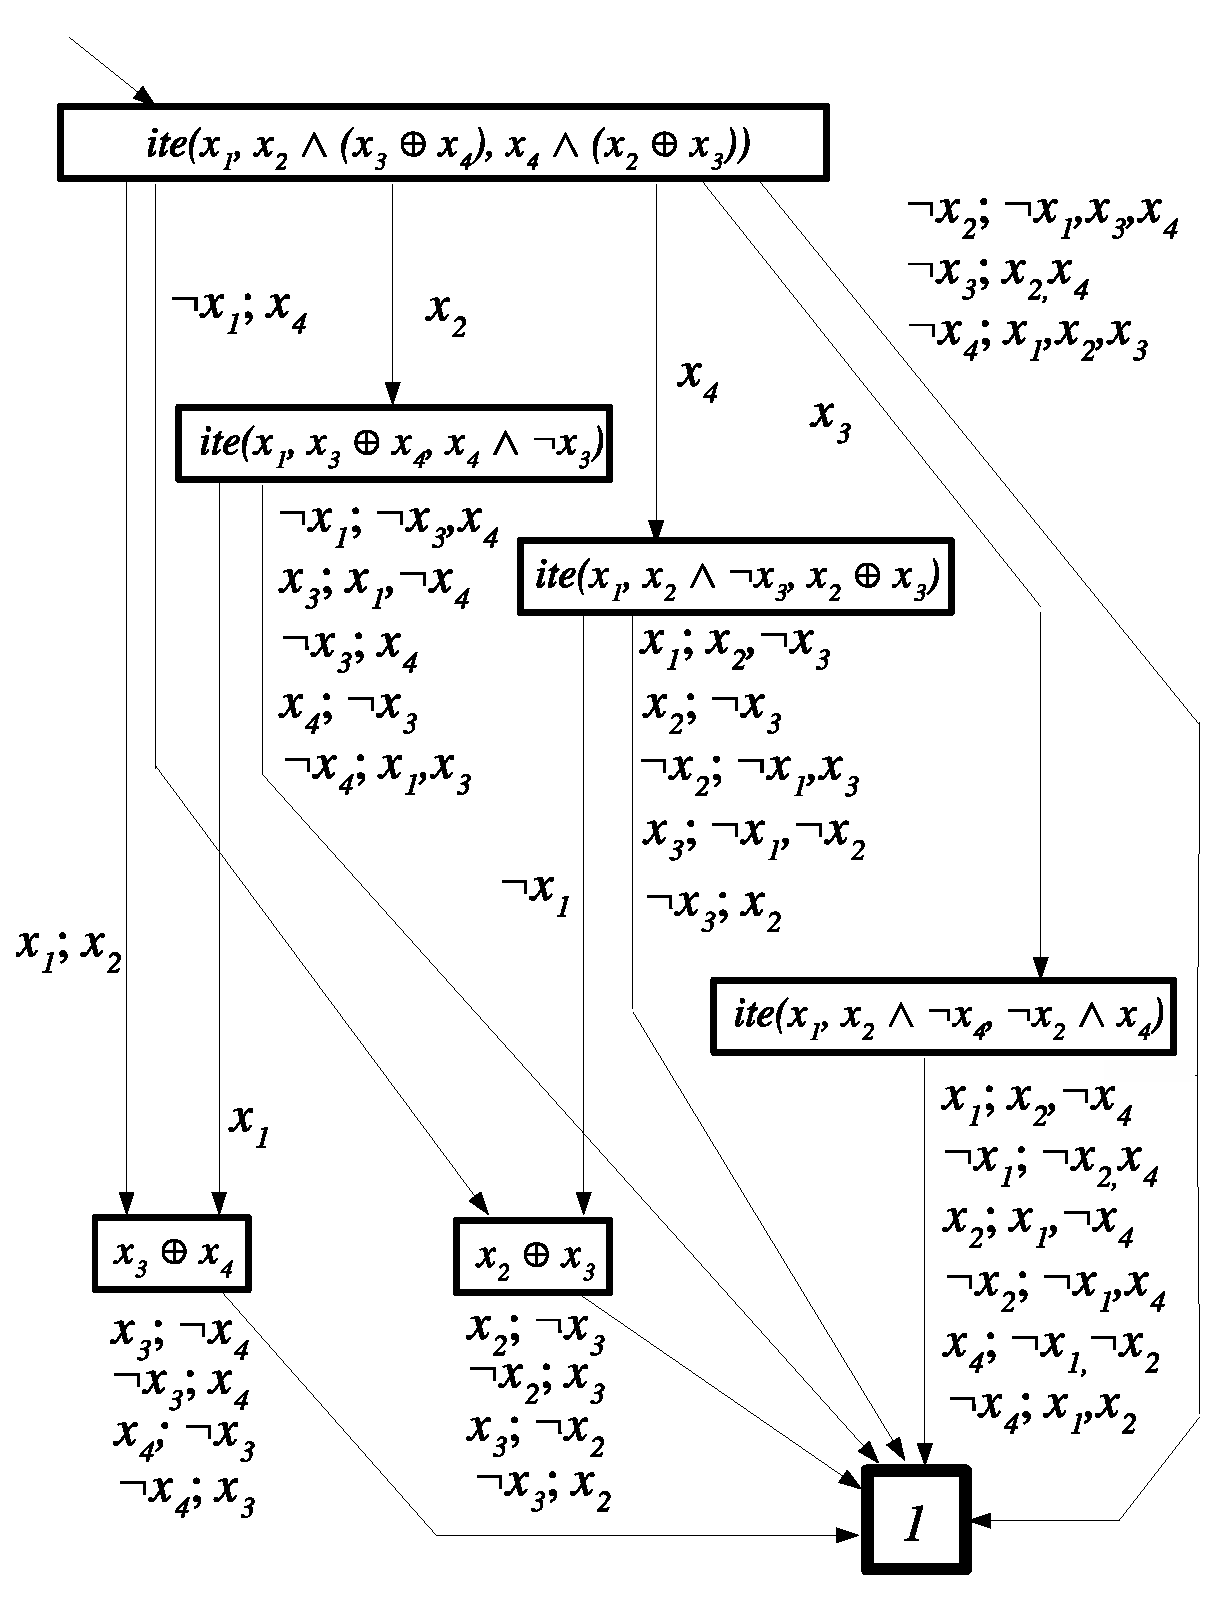
\includegraphics{Fig/smurf.eps}}
\caption{
BDDs are preprocessed into deterministic Mealy machines called ``{\sc
SMURF}s.''  This example explains construction. {\em ite\/} denotes
if-then-else and $\oplus$ denotes exclusive or.\newline\newline
The {\sc Smurf} above represents $\mbox{\sl
ite}(x_1,x_2\wedge(x_3\oplus x_4),x_4\wedge(x_2\oplus x_3))$.  It
represents, in part, BDDs for the function under
all possible variable orderings --- since we cannot know in what order
the brancher considers the variables.
\newline
The start state (upper left) represents the original function.  On the
left is a transition from the start state labeled ``$x_1;x_2$''; this
means that, from that state, on input $x_1$, the automaton makes a
transition and outputs $\{x_2\}$.  
If the brancher guesses, or infers,
that $x_1$ is true, it will ``tell'' the automaton to branch on $x_1$.
The output of $\{x_2\}$ tells the brancher that $x_2$ must also be true
--- the analogue of unit inference in CNF.  This transition goes to a
state labeled $x_3\oplus x_4$, meaning that, after $x_1,x_2$ are set
to 1, what remains to be satisfied --- the {\em residual function} ---
is $x_3\oplus x_4$.  On the upper right are three transitions shown
with one arrow.  The first is from the start state on input $\neg
x_2$; it outputs $\{\neg x_1,x_3,x_4\}$ and goes to state 1 ---
meaning the original BDD is now satisfied, {\sl i.e.}, that there is
no residual constraint to satisfy.}\label{smurf-figure}
\end{figure}

The {\sc Smurf} structure described in the figure, for a Boolean
function with $n$ variables, can have, in the worst case, close to
$3^n$ states.  Thus, an Achilles' heel of SBSAT can be handling long
input functions.  In most benchmarks, that has not been a serious
practical problem because all individual constraint are reasonably
short {\em except}\/\footnote{as In, for example, dlx benchmark suite
made available by Miroslav Velev.} for a small special group of
functions: long clauses, long exclusive disjunctions, and
``assignments'' $\lambda_0=\lambda_1\wedge\cdots\wedge\lambda_k$ and
$\lambda_0=\lambda_1\vee\cdots\vee\lambda_k$ (where the $\lambda_i$'s
are literals).  To solve the space problem for these special
functions, we create special data structures; these take little space
and can simulate the {\sc Smurf}s for the functions exactly with
little time loss.  For a long clause we store only (i) whether the
clause is already satisfied, and (ii) how many literals are currently
not assigned truth values.  Storing exclusive disjuncts is similar.
For the assignments, we store both the value ({\em 0},{\em 1}, or
unassigned) of the left-hand-side literal and the number of
right-hand-side literals with undefined truth values.

\subsection{Locally Skewed, Globally Balanced}\label{lsgb-section}

Memoized information is currently tailored for the primary search
heuristic called {\em Locally Skewed, Globally Balanced} or LSGB.  The
{\em weight} of a {\sc Smurf} transition counts the number of literals
forced on the transition, plus the expected number of literals forced
below that state, where a forced literal after $m$ additional choices
is weighted $1/K^m$.  ($K$, set experimentally, is currently 3 by
default.)  In Figure~\ref{smurf-figure}, the transition out of the
start state on $\neg x_1$ has weight
\[1+(\frac{1}{K}+\frac{1}{K}+\frac{1}{K}+\frac{1}{K})/4;\]
the transition out on $x_4$, 
\[0+(\frac{1}{K^2}+\frac{2}{K} + \frac{1}{K} + \frac{2}{K} + \frac{2}{K} +
\frac{1}{K})/6.\] 
Computing these weights is expensive but they are memoized in {\sc
Smurf}s during preprocessing and, during search, they are looked up in
a table instead of being recomputed each time they are needed.

For the special data structures defined above, the calculation above
is simulated.  If a disjunction $\lambda_1\vee\cdots\vee\lambda_m$
with $k$ still unassigned variables were represented as a {\sc Smurf},
the weight of $\lambda_i$ is 0 (since the clause immediately becomes
satisfied, nothing more can be forced), and the weight of
$\neg\lambda_i$ is $1/(2K)^{k-1}$.  This is directly coded in the
simulated {\sc Smurf}.  Exclusive disjunctions are similar.
Assignments are similar but break into cases; one recurrence relation
is hard to solve, so weights are precomputed as a function of
the number of unassigned $\lambda_i$'s and are looked up during search.

The LSGB search heuristic is similar to the ``Johnson heuristic'' on
CNF formulas where $K=2$.  The intuition is to branch toward forced
inferences as quickly as possible to narrow the search space (or get
lemmas fast).  To pick the next variable to branch on: For each
variable $x_i$, compute (i) the sum $S_i^+$ of the {\em weight}s of
transitions on $x_i$ out of all current ${\mbox{\sc Smurf}}$ states
and (ii) the sum $S_i^-$ of the {\em weight}s of transitions on $\neg
x_i$.  A high sum represents a high ``payoff.''  For an ideal
branching variable $x_i$, both $x_i$ and $\neg x_i$ force many
literals, so we branch on the variable $x_i$ where $S_i^+\cdot S_i^-$
is maximum.  For that variable, branch first toward the larger of
$S_i^+,S_i^-$.\footnote{The idea of taking the product is due to
Freeman.}

There are circumstances where other search heuristics are known to
work well.  LSGB was intended for applications where not much is known
about, or easily determined about, the given problem.  If the problem
is known to have a lot of exploitable structure, it may be better to
specify a different heuristic.  We allow the experienced user some
choice (see Sections~\ref{chaff-section}
and~\ref{user-defined-heuristic-section} below for more information).
The {\sc Smurf} structure admits such heuristics as well; on a simple
heuristic, it may not be needed, but (except for preprocessing time)
it does not hinder either.

In Section~\ref{results-section}, we present benchmark problems comparing
SBSAT with LSGB to other solvers such as zChaff.

\subsection{Chaff-like}\label{chaff-section}

\subsection{User defined search heuristic}\label{user-defined-heuristic-section}

\newpage
\section{Reference - Search methods}

\subsection{Backtracking and Lemmas}\label{lemma-section}

\subsubsection{Lemma cache}\label{lemma-section-cache}

\subsubsection{Lemma effectiveness}\label{lemma-section-effect}

\subsection{BDD WalkSAT}\label{walksat-section}

\subsection{WVF}\label{wmv-section}

\newpage
\section{Reference - Output, results}

\subsection{Raw}\label{raw-format}

If you use raw format, {\tt -R r} the output looks as follows:
\begin{verbatim}
// Solution #1
-arg1 -arg2 -arg3 -arg4 x3 x2 x1 1 2 3 -5 -bob 4 -1000 22 300 -40 -400 -50
var1 var2 var3 var4 -var5 -var6
\end{verbatim}

\subsection{Fancy}\label{fancy-format}

If you use fancy format, {\tt -R f} the output looks as follows:
\begin{verbatim}
// Solution #1
arg1     (1)    val:F
arg2     (2)    val:F
arg3     (3)    val:F
arg4     (4)    val:F
x3       (5)    val:T
x2       (6)    val:T
x1       (7)    val:T
1        (8)    val:T
2        (9)    val:T
3        (10)   val:T
5        (11)   val:F
bob      (12)   val:F
4        (13)   val:T
1000     (14)   val:F
22       (15)   val:T
300      (16)   val:T
40       (17)   val:F
400      (18)   val:F
50       (19)   val:F
var1     (20)   val:T
var2     (21)   val:T
var3     (22)   val:T
var4     (23)   val:T
var5     (24)   val:F
var6     (25)   val:F
\end{verbatim}

\newpage
\section{Reference - Data structures}

\subsection{BDD database}\label{bdd-build-section}

\subsection{{\sc Smurf}}

\subsection{Lemma database}

\newpage
\section{Reference - Results: making BDDs from {\tt bmc}}\label{the-reduction}

Among the experiments we have run, those inputs relating specifically
to bounded model checking benchmarks have been obtained from the
output of the {\tt bmc} program obtainable from Carnegie Mellon University.
That program inputs a model checking problem and a number of time
steps and outputs a propositional logic formula representing the BMC
problem in three formats: a large propositional logic formula,
three-address code representing the parse tree for that formula, and a
CNF translation of the formula.  Program {\tt bmc} internally
represents all formulas recursively as
\begin{center}
{\tt <function>} = {\tt <variable>};\\
{\tt <function>} = $\neg${\tt <variable>};\\
{\tt <function>} = {\tt <function>} {\bf op} {\tt <function>};\\
\end{center}
where {\bf op} is one of $\vee$, $\wedge$, $\to$, $\equiv$.  The
binary tree associated with such a recursion is stored as a tree of
pointers.  Each node of the tree is represented as a triple of
pointers: to the left descendent, the right descendent, and the
parent.  A pointer to the root of such a tree represents the output
formula in three-address code.  Further processing inside {\tt bmc}
converts this to a CNF expression which is also available as output.
As an example, we use {\tt bmc} to generate the three-address code 
problems for queue benchmarks (see next section) as follows:\\
\indent{\tt genqueue \# > queue\#}\\
\indent{\tt bmc -k \# queue\# -prove}\\ 
\noindent
where {\tt genqueue} is part of the {\tt bmc} suite and {\tt \#} is replaced
by a number representing problem complexity.  The CNF versions are 
created by replacing the last line above with this:\\
\indent{\tt bmc -k \# queue\# -dimacs}

\noindent
We use {\tt bmc} to generate three-address and CNF inputs directly,
instead of taking already generated CNF formulas ``off the shelf'' so
we have equivalent three-address and CNF data.  Thus,
times we report for zChaff, Berkmin, and Siege may differ from
published times.

The largest propositional logic formula output by {\tt bmc} is a
conjunction of smaller formulas, so the obvious course for SBSAT is to
read in each of those smaller formulas as a BDD.  Nevertheless, for
some of the {\tt bmc} outputs, those propositional logic formulas were
much too large even to store as BDDs.  Of course, we also did not want
to use the three-address code or the CNF representation directly,
since that would negate the benefits of {\sc Smurf}s which are to
retain potentially exploitable domain-specific relationships.  Our
current approach is successful in spite of being amazingly simplistic.
\begin{enumerate}
\item We read in the three-address code and recreate the large
      propositional formula so as not to lose domain-specific 
      information.  Starting at the bottom of this formula
      we start building a BDD.  We use a greedy algorithm: when 
      the BDD gets too large (10-18 variables) we insert a new 
      variable to represent the BDD so far, include a BDD
      asserting that is what the new variable represents, replace the
      part we have translated with the new variable, and continue the
      process.  
      %Obviously, this translation does not capture all
      %subtle relationships of the input BMC problem.  
      This particular translation goes against our intention of
      staying in the original domain, however, this simple process 
      still proves useful. In future research we hope to find a better 
      algorithm.  
\item To break each resultant BDD $f$ down to a 10-variable maximum
      (so that the {\sc Smurf}s remain suitably small), we do the
      following (see also Section~\ref{splitter-section}):

      (a) Compute all projections $f_i$ of the BDD onto 10-variable
      subsets of its variable set  (see
      Section~\ref{strengthening-section} for the meaning of projection).

      (b) Simplify the $f_i$'s against each other
      and delete resultant $f_i$'s which
      become {\tt True}.  Below we call the final simplified $f_i$'s
      $f_1,\ldots,f_k$.

      Note that $f$ logically implies each $f_i$; we can think of them
      as ``approximations'' to $f$, in the sense that each is false on
      some, but probably not all, of the truth assignments on which
      $f$ is false.

      (c) Recall that the goal is to replace $f$ with a set of smaller
      BDD's.  Now $f$ is logically equivalent to the conjunction of
      the set $\{f_1,f_2,\ldots,f_k,f^\star\}$ where
\[f^\star=(f_1\wedge f_2\wedge \cdots \wedge f_k)\rightarrow f\]
      ($f^\star$ just excludes the truth assignments where all the
      $f_i$'s are true but $f$ is is false).

      If $f^\star$ has $\le 10$ variables, we replace $f$ with
      $\{f_1,f_2,\ldots,f_k,f^\star\}$.  If $f^\star$ has $>10$
      variables, we replace $f$ with $\{f_1,f_2,\ldots,f_k\}$ plus the
      translation of $f^\star$ to CNF.  (Typically, $f^\star$ is
      satisfied in most truth assignments, so its CNF translation
      should be fairly short.)

      Again, this procedure is simplistic.  We hope in the future to
      find a better algorithm.
\end{enumerate}

\newpage
\section{Reference - Results: Experiments}\label{results-section}

SBSAT was tested on several popular benchmark suites.  We also ran
current versions of Berkmin (v.\ 561), zChaff (v.\ 2003.10.9), and
Siege (v.\ 4) on these benchmarks for comparison.  In addition, we
concocted a class of random problems, called {\em sliders}, which
resemble BMC problems in that copies of the same function, each
differing only in the input variables it depends on, are conjoined.
Making those functions random, in some sense, makes sliders hard.
Specifically, sliders are defined as follows:\\

\parbox{4.5in}{ Choose $m$, even, the number of constraints and the
number of variables.  Choose $k$, and $l$, the number of variables
input to constraint functions.  Choose constraint functions
$f(x_1,x_{i_1},...,x_{i_{k-2}},x_{m/2})$ and
$g(x_1,x_{j_1},...,x_{j_{l-2}},x_{m/2})$, with variables explicitly
listed, in increasing order of subscript, and $k$ and $l$ are small 
compared to $m$.  Form the constraint set
\begin{eqnarray*}
&&\{f(x_{1+h},x_{i_1+h},...,x_{i_{k-2}+h}, x_{(m/2)+h}): 0\leq h\leq m/2\}\cup\\
&&\{g(x_{1+h},x_{j_1+h},...,x_{j_{l-2}+h}, x_{(m/2)+h}) = o_h: 0\leq
h\leq m/2\}
\end{eqnarray*}
where each $o_h$ is independently and uniformly chosen from $\{0,1\}$.
} 

\noindent
We find sliders appealing because they resemble some real-world
problem domains and because $f$ and $g$ can be designed to force
inferences to occur only when nearly all inputs of $f$ and $g$ are
assigned values.  This fact makes conflict analysis useless, and is
challenging to a search heuristic which is looking for information
contained in groups of variables.

At this stage of our SBSAT implementation, lemmas are
handled in a rather primitive manner so we observe an unusually low
number of backtracks per second.  All experiments were run on a single
processor Pentium 4, 2 GHz, with 2 GB RAM.

Our first set of results, shown in Table~\ref{longMultTable}, is for
the problem of verifying a long multiplier.  The circuit definition is
available from Carnegie Mellon University.  All inputs are unsatisfiable.
The left column of the table shows the number of time steps involved
in the verification of each benchmark (see
Section~\ref{the-reduction}).  Experiments were run from 4 time steps
to 70 time steps.  The next three columns present the observed
performance of SBSAT on three-address inputs in total number of choice
points, total time, and search time.  The next three columns present
the same information except when translated CNF formulas are input
(see Section~\ref{the-reduction}).  The next two columns present the
performance of zChaff in choice points and total time and the last two
columns present the results of Siege and Berkmin on the CNF versions
we generated.

\begin{table}
\centerline{\tiny
\begin{tabular}{|c||r|r|r||r|r|r||r|r|r|r|}\hline
& \multicolumn{3}{c||}{SBSAT on Three-Address} 
& \multicolumn{3}{c||}{SBSAT on CNF}
& \multicolumn{2}{c|}{zChaff on CNF}
& \multicolumn{1}{c|}{Siege}
& \multicolumn{1}{c|}{Berkmin}\\\hline
\multicolumn{1}{|c||}{\#time} &  
\multicolumn{1}{c|}{number} & 
\multicolumn{1}{c|}{total}  & 
\multicolumn{1}{c||}{branch} & 
\multicolumn{1}{c|}{number} & 
\multicolumn{1}{c|}{total}  & 
\multicolumn{1}{c||}{branch} & 
\multicolumn{1}{c|}{number} & 
\multicolumn{1}{c|}{total} &
\multicolumn{1}{c|}{total} & 
\multicolumn{1}{c|}{total} \\
\multicolumn{1}{|c||}{steps} & 
\multicolumn{1}{c|}{choices} & 
\multicolumn{1}{c|}{(sec)} & 
\multicolumn{1}{c||}{(sec)} & 
\multicolumn{1}{c|}{choices} & 
\multicolumn{1}{c|}{(sec)} & 
\multicolumn{1}{c||}{(sec)} & 
\multicolumn{1}{c|}{choices} & 
\multicolumn{1}{c|}{(sec)} &
\multicolumn{1}{c|}{(sec)} & 
\multicolumn{1}{c|}{(sec)} \\\hline\hline
4  &   720 &   2.3 &  0.16 &   687 &  1.47 &  0.86 &   1041 &  0.45 &
0.2 & 0.27\\  
8  & 10000 & 14.78 &  7.12 & 13110 & 41.02 & 39.28 &  33272 & 50.37 &
12.73 & 18.9 \\  
12 & 19398 & 42.14 & 27.31 & 31963 & 167.8 & 163.8 & 122522 & 357.1 &
71.61 & 96.9 \\  
16 & 17508 & 61.05 & 38.89 & 32969 & 247.3 & 240.4 & 125026 & 366.7 &
177.4 & 200.6 \\
20 & 14077 & 72.63 & 41.65 & 34426 & 347.0 & 335.1 & 164373 & 585.9 &
165.2 & 178.8 \\
24 & 17775 & 118.5 & 77.03 & 23854 & 270.0 & 252.0 & 214263 & 790.3 &
542.8 & 312.2 \\  
28 & 18872 & 134.1 & 81.71 & 23847 & 319.0 & 293.8 & 220045 & 888.2 &
805.4 & 255.0 \\  
32 & 18538 & 155.6 & 90.5  & 16718 & 262.9 & 228.3 & 216916 & 882.8 &
1035 & 334.6 \\  
36 & 20356 & 186.8 & 109.9 & 14750 & 278.0 & 233.5 & 269856 & 1055 &
576.8 & 420.4 \\ 
40 & 19141 & 203.3 & 113.5 & 11703 & 281.1 & 225.0 & 289687 & 1103 &
845.3 & 442.6 \\
50 & 21867 & 263.0 & 134.4 & 11306 & 378.6 & 286.9 & 472053 & 2032 &
1552 & 466.9 \\
60 & 24985 & 434.1 & 239.4 & 10844 & 450.2 & 313.6 & 461867 & 2183 &
3340 & 709.2 \\
70 & 26907 & 618.4 & 335.9 & 11270 & 632.8 & 164.3 & 850942 & 5875 &
2860 & 844.7 \\
\hline
\end{tabular}}
\caption{SBSAT, zChaff, Siege, Berkmin times on the Long Multiplier benchmarks}
\label{longMultTable}
\end{table}

Observe that SBSAT working in the user domain on three-address code
shows a slight advantage to working with the CNF translation.  It is
interesting that in the case of CNF inputs, more preprocessing seems
to result in less searching.  The fact that preprocessing varies so
much from benchmark to benchmark on CNF inputs may reflect the
imprecision of guesses made when trying to recreate domain-specific
information from given CNF formulas.  Such preprocessing fluctuations
are not as pronounced when three-address codes are input to SBSAT.

Observe that zChaff and Siege cannot compete with SBSAT on long
multiplier benchmarks.  The problem seems to be due to encountering
many more choicepoints during search.  Berkmin visits only about an
order of magnitude more choicepoints than SBSAT on CNF inputs but the
slower implementation of lemmas in SBSAT enables Berkmin to be only a
fraction slower than SBSAT, in general.  The difference in
choicepoints suggests the success in this case is due to the complex
search heuristic used natively in SBSAT.

Table~\ref{barrel} shows timings for the set of barrel
benchmarks.  The three-address code equivalents were generated by
applying the {\tt bmc} tool to the output of the {\tt genbarrel}
utility in the {\tt bmc} suite.  All inputs are unsatisfiable.  Runs
were cut off prematurely if not completed before 3600 seconds.  This
is reflected as a line (---) through a table entry.
%The --- symbols
%indicate that the run was aborted at maximum time, which was 1000
%seconds.
%For the smallest cases, 2-4 time steps, zChaff on the {\tt
%bmc} CNF output was fastest; for 5-6 time steps, SBSAT on the CNF
%output was fastest, and for 7-9 time steps SBSAT for the BDDs
%assembled from the {\tt bmc} 3-address code was fastest. 

Observe that in all cases, SBSAT solved the problems constructed from
the three-address code without any search.  This raises the question
of whether a BDD tool might also do as well.  This appears not to be
the case, since we build a collection of BDDs of about 10 variables
each and then strengthen them against each other.  The inferences
resulting from this process are enough to generate a contradiction
before search is applied.  We suppose a BDD tool would either have
attempted to build a single BDD from the three-address code, in which
case it would have been forced to give up due to unmanageable sizes,
or it would have used the conjoin operation instead of the
strengthening operation to combine the BDDs, probably again taking too
much space.  Although the time taken by SBSAT in preprocessing is
considerable, it is shown to be well-spent as SBSAT, zChaff, Siege,
and Berkmin all have difficulty with the larger CNF versions of the
barrel benchmarks.  Thus, it appears staying closer to the user-domain
and preprocessing to reveal inferences early has paid off on these 
benchmarks.

\begin{table}
\centerline{\tiny
\begin{tabular}{|c||c|c|c||c|c|c||c|c|c|c|}\hline
& \multicolumn{3}{c||}{SBSAT on Three-Address} 
& \multicolumn{3}{c||}{SBSAT on CNF}
& \multicolumn{2}{c|}{zChaff on CNF}
& \multicolumn{1}{c|}{Siege}
& \multicolumn{1}{c|}{Berkmin}\\\hline
\multicolumn{1}{|c||}{Name} &
\multicolumn{1}{c|}{number} &
\multicolumn{1}{c|}{total} &
\multicolumn{1}{c||}{branch} &
\multicolumn{1}{c|}{number} &
\multicolumn{1}{c|}{total} &
\multicolumn{1}{c||}{branch} &
\multicolumn{1}{c|}{number} &
\multicolumn{1}{c|}{total} &
\multicolumn{1}{c|}{total} &
\multicolumn{1}{c|}{total} \\
\multicolumn{1}{|c||}{} & 
\multicolumn{1}{c|}{choices} & 
\multicolumn{1}{c|}{(sec)} & 
\multicolumn{1}{c||}{(sec)} & 
\multicolumn{1}{c|}{choices} & 
\multicolumn{1}{c|}{(sec)} & 
\multicolumn{1}{c||}{(sec)} & 
\multicolumn{1}{c|}{choices} & 
\multicolumn{1}{c|}{(sec)} &
\multicolumn{1}{c|}{(sec)} &
\multicolumn{1}{c|}{(sec)} \\\hline\hline
barrel2  & 0 &  0.00 & 0.00 &    3 &  0.05 &  0.00 &       3 &  0.00 & 0.01
& 0.0 \\
barrel3  & 0 &  0.11 & 0.00 &   13 &  0.08 &  0.00 &      48 &  0.00 & 0.01 
& 0.0 \\
barrel4  & 0 &  0.12 & 0.00 &   33 &  0.15 &  0.01 &     201 &  0.02 & 0.01
& 0.01 \\
barrel5  & 0 &  0.72 & 0.00 &  354 &  0.66 &  0.21 &    8856 &  0.58 & 0.67
& 0.65 \\
barrel6  & 0 &  1.48 & 0.00 & 1205 &  2.89 &  1.96 &   28110 &  2.81 & 5.97
& 5.56 \\
barrel7  & 0 &  2.84 & 0.00 & 2848 & 11.10 &  8.51 &   66959 & 11.37 & 21.19
& 29.96 \\
barrel8  & 0 &  5.05 & 0.00 & 4304 & 25.15 & 18.71 &  116858 & 31.98 & 136.7
& 298.3 \\
barrel9  & 0 & 67.87 & 0.00 & ---  & ---   & ---   &  649532 & 254.6 & 41.24
& 89.27 \\
barrel10 & 0 & 108.9 & 0.00 & ---  & ---   & ---   & 1801476 & 1191  & 86.34
& 184.0 \\
barrel11 & 0 & 166.2 & 0.00 & ---  & ---   & ---   & ---     & ---   & 134.7
& 238.3 \\
barrel12 & 0 & 243.8 & 0.00 & ---  & ---   & ---   & ---     & ---   & 927.1
& 999.3 \\
barrel13 & 0 & 348.4 & 0.00 & ---  & ---   & ---   & ---     & ---   & 629.9
& 1049 \\
barrel14 & 0 & 481.9 & 0.00 & ---  & ---   & ---   & ---     & ---   & 2122
& 3389 \\
barrel15 & 0 & 655.9 & 0.00 & ---  & ---   & ---   & ---     & ---   & ---
& ---  \\
barrel16 & 0 & 859.7 & 0.00 & ---  & ---   & ---   & ---     & ---   & ---
& ---  \\
\hline
\end{tabular}}
\caption{SBSAT, zChaff, Siege, Berkmin times on the Barrel benchmarks}
\label{barrel}
\end{table}

Tables~\ref{QueueTable}~and~\ref{PermuteTable} show
timings for a set of queue benchmarks and permute benchmarks generated
by {\tt genqueue} and {\tt genpermute}, respectively, from the {\tt
bmc} suite.  Cutoff of runs was set at 3600 seconds for the queue
benchmarks and 60000 seconds for the permute benchmarks.  All inputs
are unsatisfiable.  The pattern observed is similar to the previous
sets of runs.  When SBSAT works with three-address code timings are
much better than when equivalent CNF inputs are used.  Working in
three-address code gets results faster than other solvers on
equivalent CNF inputs.

\begin{table}
\centerline{\tiny
\begin{tabular}{|c||c|c|c||c|c|c||c|c|c|c|}\hline
& \multicolumn{3}{c||}{SBSAT on Three-Address} 
& \multicolumn{3}{c||}{SBSAT on CNF}
& \multicolumn{2}{c|}{zChaff on CNF}
& \multicolumn{1}{c|}{Siege}
& \multicolumn{1}{c|}{Berkmin}\\\hline
\multicolumn{1}{|c||}{Name} &
\multicolumn{1}{c|}{number} &
\multicolumn{1}{c|}{total} &
\multicolumn{1}{c||}{branch} &
\multicolumn{1}{c|}{number} &
\multicolumn{1}{c|}{total} &
\multicolumn{1}{c||}{branch} &
\multicolumn{1}{c|}{number} &
\multicolumn{1}{c|}{total} &
\multicolumn{1}{c|}{total} &
\multicolumn{1}{c|}{total} \\
\multicolumn{1}{|c||}{} &  
\multicolumn{1}{c|}{choices} & 
\multicolumn{1}{c|}{(sec)} & 
\multicolumn{1}{c||}{(sec)} & 
\multicolumn{1}{c|}{choices} & 
\multicolumn{1}{c|}{(sec)} & 
\multicolumn{1}{c||}{(sec)} & 
\multicolumn{1}{c|}{choices} & 
\multicolumn{1}{c|}{(sec)} &
\multicolumn{1}{c|}{(sec)} &
\multicolumn{1}{c|}{(sec)} \\ \hline\hline
queue4  &       41 &  0.1 &  0.0 &     19 & 0.11 & 0.00 &    32 & 0.00
& 0.01 & 0.0 \\  
queue8  &      651 & 3.04 & 0.07 &    291 & 0.49 & 0.10 &   561 & 0.05
& 0.04 & 0.05 \\  
queue12 &     4351 & 5.53 & 1.02 &   3875 & 5.52 & 4.38 & 11752 & 3.09
& 1.04 & 0.96 \\
queue16 &    30835 & 22.3 & 14.7 &  41029 &  107 &  104 & 73407 & 62.22 
& 30.27 & 32.38 \\
queue20 &   311127 &  265 &  227 & 565559 & 2420 & 2412 & 698914 & 1874 
& 400.4 & 401.0 \\
queue22 &  1052750 &  843 &  798 & 2016859 & 9367 & 9356 & --- & --- 
& 1886 & 1050 \\
queue24 &  3262464 & 2666 & 2613 & ---   & --- & --- & ---  & --- 
& --- & 2724 \\  
\hline
\end{tabular}
}
\caption{SBSAT, zChaff, Siege, Berkmin times on the Queue benchmarks}
\label{QueueTable}
\end{table}

\begin{table}
\centerline{\tiny
\begin{tabular}{|c||c|c|c||c|c|c||c|c|c|c|}\hline
& \multicolumn{3}{c||}{SBSAT on Three-Address} 
& \multicolumn{3}{c||}{SBSAT on CNF}
& \multicolumn{2}{c|}{zChaff on CNF}
& \multicolumn{1}{c|}{Siege}
& \multicolumn{1}{c|}{Berkmin}\\\hline
\multicolumn{1}{|c||}{Name} &
\multicolumn{1}{c|}{number} &
\multicolumn{1}{c|}{total} &
\multicolumn{1}{c||}{branch} &
\multicolumn{1}{c|}{number} &
\multicolumn{1}{c|}{total} &
\multicolumn{1}{c||}{branch} &
\multicolumn{1}{c|}{number} &
\multicolumn{1}{c|}{total} &
\multicolumn{1}{c|}{total} &
\multicolumn{1}{c|}{total} \\
\multicolumn{1}{|c||}{} &  
\multicolumn{1}{c|}{choices} & 
\multicolumn{1}{c|}{(sec)} & 
\multicolumn{1}{c||}{(sec)} & 
\multicolumn{1}{c|}{choices} & 
\multicolumn{1}{c|}{(sec)} & 
\multicolumn{1}{c||}{(sec)} & 
\multicolumn{1}{c|}{choices} & 
\multicolumn{1}{c|}{(sec)} &
\multicolumn{1}{c|}{(sec)} &
\multicolumn{1}{c|}{(sec)} \\ \hline\hline
permute2  &       0 & 0.01 & 0.00 &   1 & 0.05 & 0.00 &  1 & 0.00
& 0.01 & 0.00 \\  
permute3  &       5 & 0.04 & 0.00 &   14 & 0.07 & 0.00 &  11 & 0.00
& 0.01 & 0.00 \\  
permute4  &      68 & 0.65 & 0.00 &   47 & 0.11 & 0.00 &  52 & 0.00
& 0.01 & 0.01 \\  
permute5  &     174 & 10.1 & 0.01 &  304 & 0.27 & 0.10 &  199 & 0.02
& 0.02 & 0.03 \\  
permute6  &     893 & 11.46 & 0.09 & 1655 & 1.44 & 1.15 &  2021 & 0.28
& 0.17 & 0.16 \\  
permute7  &    5537 & 23.24 & 0.81 & 8551 & 9.21 & 8.77 &  16485 & 9.51
& 2.88 & 1.12 \\  
permute8  &   64607 & 71.16 & 70.21 & 58051 & 244.1 & 243.2 & 110492 & 172.93
& 21.6 & 15.7 \\  
permute9  &  454726 & 686.6 & 685.0 & 471422 & 2575 & 2573 & 361422 & 1018
& 315 & 228 \\  
permute10  & 1311291 & 2064 & 2062 & --- & --- & --- & 2118409 & 12101
& 3003 & 3891 \\  
permute11  & 20462503 & 39260 & 39257 & --- & --- & --- & --- & ---
& --- & --- \\  
\hline
\end{tabular}
}
\caption{SBSAT, zChaff, Siege, Berkmin times on the Permute benchmarks}
\label{PermuteTable}
\end{table}

The story changes on the queue invariant benchmarks of
Table~\ref{QueueInvTable}.  In this case, SBSAT experienced memory
problems.  In order to fit the resulting {\sc Smurf}s into memory, the
BDDs upon which they were based were required to be so small we had to
change their maximum size manually, that is, after preprocessing.  The
result was an unexpectedly large amount of garbling of domain-specific
information and dismal results.  We did not feel it was worthwhile
reporting them.  Although SBSAT did solve the CNF versions of these
problems, the other solvers performed better as in previous benchmark
sets.

\begin{table}
\centerline{\tiny
\begin{tabular}{|c||c|c|c||c|c|c|c|}\hline
& \multicolumn{3}{c||}{SBSAT on CNF}
& \multicolumn{2}{c|}{zChaff on CNF}
& \multicolumn{1}{c|}{Siege}
& \multicolumn{1}{c|}{Berkmin}\\\hline
\multicolumn{1}{|c||}{Name} &
\multicolumn{1}{c|}{number} &
\multicolumn{1}{c|}{total} &
\multicolumn{1}{c||}{branch} &
\multicolumn{1}{c|}{number} &
\multicolumn{1}{c|}{total} &
\multicolumn{1}{c|}{total} &
\multicolumn{1}{c|}{total} \\
\multicolumn{1}{|c||}{} &  
\multicolumn{1}{c|}{choices} & 
\multicolumn{1}{c|}{(sec)} & 
\multicolumn{1}{c||}{(sec)} & 
\multicolumn{1}{c|}{choices} & 
\multicolumn{1}{c|}{(sec)} &
\multicolumn{1}{c|}{(sec)} &
\multicolumn{1}{c|}{(sec)} \\ \hline\hline
queueinv4  &       83 &  0.08 &  0.01 &    136 &  0.00 & 0.01 & 0.01 \\  
queueinv8  &      438 &  0.17 &  0.07 &   1122 &  0.04 & 0.06 & 0.06 \\  
queueinv12 &     1429 &  0.98 &  0.42 &   4368 &  0.22 & 0.31 & 0.12 \\
queueinv16 &     2411 &  1.04 &  0.75 &   7721 &  0.27 & 0.53 & 0.24 \\
queueinv20 &     4787 &  6.81 &  2.91 &  16258 &  1.63 & 0.73 & 0.81 \\
queueinv24 &     7379 & 13.62 &  6.00 &  26995 &  2.96 & 1.89 & 1.90 \\  
queueinv28 &    10914 & 25.61 & 11.23 &  38145 &  5.69 & 3.88 & 3.40 \\
queueinv32 &    15403 & 16.73 & 14.56 &  68641 &  3.20 & 3.74 & 4.20 \\  
queueinv36 &    21324 & 116.6 & 35.01 & 103281 & 23.58 & 9.59 & 10.33 \\  
queueinv40 &    27404 & 189.2 & 52.54 & 145691 & 38.08 & 17.62 & 16.46 \\  
queueinv44 &    35820 & 309.2 & 88.65 & 166634 & 46.42 & 57.38 & 25.16 \\  
queueinv48 &    44719 & 476.2 & 135.8 & 217615 & 79.95 & 62.0 & 43.61 \\  
queueinv52 &    52320 & 683.8 & 189.9 & 297830 & 179.2 & 155.5 & 55.93 \\  
queueinv56 &    51768 & 928.0 & 238.9 & 397142 & 239.1 & 514.9 & 82.13 \\  
\hline
\end{tabular}
}
\caption{SBSAT, zChaff, Siege, Berkmin times on the Queue Invariant benchmarks}
\label{QueueInvTable}
\end{table}

For completeness, we include results on the dlx suite available from
Carnegie Mellon University in Table~\ref{dlxTable}.  Some inputs are
satisfiable and some are unsatisfiable.  We applied SBSAT to two
variations: namely Trace and CNF formats (both available).  All
problems in this suite are easy for all the solvers and that is about
all that can be said about them.  We did not include results of dlx9
benchmarks because SBSAT had some memory problems.

\begin{table}
\centerline{\tiny
\begin{tabular}{|l||r|r|r||r|r|r||r|r|r|c|}\hline
& \multicolumn{3}{c||}{SBSAT on Trace} 
& \multicolumn{3}{c||}{SBSAT on CNF}
& \multicolumn{2}{c|}{zChaff on CNF}
& \multicolumn{1}{c|}{Siege}
& \multicolumn{1}{c|}{Berkmin}\\\hline
\multicolumn{1}{|c||}{Name} &  
\multicolumn{1}{c|}{number} & 
\multicolumn{1}{c|}{total}  & 
\multicolumn{1}{c||}{branch} & 
\multicolumn{1}{c|}{number} & 
\multicolumn{1}{c|}{total}  & 
\multicolumn{1}{c||}{branch} & 
\multicolumn{1}{c|}{number} & 
\multicolumn{1}{c|}{total} &
\multicolumn{1}{c|}{total} & 
\multicolumn{1}{c|}{total} \\
\multicolumn{1}{|c||}{} & 
\multicolumn{1}{c|}{choices} & 
\multicolumn{1}{c|}{(sec)} & 
\multicolumn{1}{c||}{(sec)} & 
\multicolumn{1}{c|}{choices} & 
\multicolumn{1}{c|}{(sec)} & 
\multicolumn{1}{c||}{(sec)} & 
\multicolumn{1}{c|}{choices} & 
\multicolumn{1}{c|}{(sec)} &
\multicolumn{1}{c|}{(sec)} & 
\multicolumn{1}{c|}{(sec)} \\\hline\hline
dlx1\_c  &  525 & 0.12 & 0.02 &  592 & 0.12 & 0.03 &  1082 & 0.02 &
0.01 & 0.01\\  
dlx2\_aa & 1755 & 0.22 & 0.06 & 2062 & 0.26 & 0.08 &  5224 & 0.10 &
0.06 & 0.02 \\  
dlx2\_ca & 7247 & 1.49 & 1.00 & 6861 & 1.60 & 0.91 &  9800 & 0.30 &
0.17 & 0.12 \\  
dlx2\_cc & 9655 & 2.60 & 2.03 & 9631 & 2.83 & 1.97 & 17825 & 0.95 &
0.36 & 0.26 \\
dlx2\_cl & 9375 & 2.14 & 1.56 & 8872 & 2.33 & 0.57 & 25390 & 1.50 &
0.71 & 0.29 \\
dlx2\_cs & 8489 & 1.84 & 1.31 & 7916 & 2.15 & 1.37 & 16310 & 0.77 &
0.20 & 0.23 \\  
dlx2\_la & 6233 & 1.06 & 0.64 & 6814 & 1.41 & 0.84 &  9246 & 0.26 &
0.11 & 0.10 \\  
dlx2\_sa & 2938 & 0.35 & 0.16 & 2168 & 0.38 & 0.15 &  5563 & 0.14 &
0.08 & 0.03 \\  
\hline
dlx2\_cc\_bug01 & 6603 & 1.77 & 1.20 & 6448 & 2.11 & 1.25 & 14471 & 0.84 &
0.18 & 0.28 \\ 
dlx2\_cc\_bug02 & 6584 & 1.80 & 1.22 & 6432 & 2.09 & 1.25 & 13717 & 0.79 &
0.48 & 0.26 \\
dlx2\_cc\_bug03 & 6861 & 1.81 & 1.23 & 6628 & 2.09 & 1.23 & 22776 & 1.05 &
0.01 & 0.10 \\
dlx2\_cc\_bug04 & 6932 & 1.92 & 1.33 & 6699 & 1.12 & 1.28 & 12860 & 0.52 &
0.08 & 0.08 \\
dlx2\_cc\_bug05 & 3743 & 1.24 & 0.65 & 3413 & 1.47 & 0.62 &   376 & 0.01 &
0.22 & 0.13 \\
dlx2\_cc\_bug06 & 3630 & 1.19 & 0.60 & 3581 & 1.52 & 0.67 &   374 & 0.01 &
0.01 & 0.10 \\
dlx2\_cc\_bug07 & 4601 & 1.36 & 0.77 & 3567 & 1.50 & 0.65 &   316 & 0.01 &
0.03 & 0.05 \\
dlx2\_cc\_bug08 & 5964 & 1.65 & 1.06 & 5353 & 1.75 & 0.92 &   747 & 0.02 &
0.01 & 0.04 \\
dlx2\_cc\_bug09 & 2549 & 0.92 & 0.42 & 2693 & 1.18 & 0.33 &   321 & 0.01 &
0.01 & 0.02 \\
dlx2\_cc\_bug10 & 3423 & 1.15 & 0.55 & 3564 & 1.41 & 0.56 &   259 & 0.00 &
0.02 & 0.02 \\
dlx2\_cc\_bug11 & 6037 & 1.60 & 1.03 & 6886 & 2.20 & 1.35 & 10528 & 0.43 &
0.02 & 0.06 \\
dlx2\_cc\_bug12 & 7099 & 2.00 & 1.43 & 5702 & 1.91 & 1.05 & 11099 & 0.44 &
0.07 & 0.10 \\
dlx2\_cc\_bug13 & 5998 & 1.69 & 1.12 & 6133 & 1.91 & 1.08 & 12049 & 0.50 &
0.03 & 0.02 \\
dlx2\_cc\_bug14 &  253 & 0.59 & 0.01 &  298 & 0.87 & 0.01 &   234 & 0.01 &
0.12 & 0.02 \\
dlx2\_cc\_bug15 & 4405 & 1.93 & 1.27 & 3756 & 1.99 & 0.99 &   296 & 0.01 &
0.01 & 0.06 \\
dlx2\_cc\_bug16 &  252 & 0.58 & 0.01 &  297 & 0.86 & 0.01 &   233 & 0.01 &
0.13 & 0.01 \\
dlx2\_cc\_bug17 &  504 & 1.16 & 0.06 & 4453 & 2.97 & 1.01 &  5806 & 0.40 &
0.01 & 0.01 \\
dlx2\_cc\_bug18 & 1066 & 1.06 & 0.10 & 3236 & 2.51 & 0.78 &   337 & 0.01 &
0.01 & 0.02 \\
dlx2\_cc\_bug19 &  269 & 0.63 & 0.02 &  302 & 0.89 & 0.02 &  4452 & 0.15 &
0.01 & 0.00 \\
dlx2\_cc\_bug20 &  703 & 0.60 & 0.03 &  777 & 0.89 & 0.50 &   521 & 0.01 &
0.01 & 0.02 \\
dlx2\_cc\_bug21 &  331 & 0.59 & 0.02 &  360 & 0.85 & 0.02 &   458 & 0.01 &
0.01 & 0.01 \\
dlx2\_cc\_bug22 &  744 & 0.62 & 0.40 &  865 & 0.91 & 0.05 &  4456 & 0.19 &
0.01 & 0.04 \\
dlx2\_cc\_bug23 &  620 & 0.60 & 0.03 &  323 & 0.86 & 0.02 &  4726 & 0.14 &
0.01 & 0.10 \\
dlx2\_cc\_bug24 &  270 & 0.59 & 0.02 &  313 & 0.86 & 0.02 &  4034 & 0.14 &
0.01 & 0.04 \\
dlx2\_cc\_bug25 & 3931 & 1.32 & 0.75 & 3233 & 1.44 & 0.59 &  4406 & 0.14 &
0.01 & 0.02 \\
dlx2\_cc\_bug26 & 4200 & 1.42 & 0.83 & 3687 & 1.58 & 0.48 &   543 & 0.02 &
0.02 & 0.02 \\
dlx2\_cc\_bug27 &  591 & 0.52 & 0.02 & 2979 & 1.16 & 0.46 &   293 & 0.01 &
0.03 & 0.00 \\
dlx2\_cc\_bug28 & 2205 & 0.88 & 0.22 & 5275 & 2.05 & 1.09 &   339 & 0.01 &
0.08 & 0.01 \\
dlx2\_cc\_bug29 &  324 & 0.58 & 0.01 &  334 & 0.87 & 0.02 &   243 & 0.01 &
0.19 & 0.03 \\
dlx2\_cc\_bug30 &  311 & 0.60 & 0.02 &  267 & 0.89 & 0.02 &   323 & 0.01 &
0.30 & 0.02 \\
dlx2\_cc\_bug31 &  294 & 0.58 & 0.02 &  325 & 0.88 & 0.02 &   247 & 0.00 &
0.24 & 0.02 \\
dlx2\_cc\_bug32 &  278 & 0.59 & 0.02 &  317 & 0.86 & 0.02 &   242 & 0.00 &
0.02 & 0.01 \\
dlx2\_cc\_bug33 &  299 & 0.58 & 0.02 &  305 & 0.88 & 0.02 &   272 & 0.01 &
0.19 & 0.06 \\
dlx2\_cc\_bug34 &  329 & 0.60 & 0.02 &  506 & 0.86 & 0.03 &   298 & 0.01 &
0.30 & 0.02 \\
dlx2\_cc\_bug35 &  282 & 0.59 & 0.02 &  328 & 0.89 & 0.02 &   318 & 0.01 &
0.32 & 0.03 \\
dlx2\_cc\_bug36 &  279 & 0.61 & 0.02 &  325 & 0.86 & 0.02 &   316 & 0.01 &
0.08 & 0.07 \\
dlx2\_cc\_bug37 & 3643 & 1.28 & 0.71 & 3214 & 1.45 & 0.60 &   329 & 0.01 &
0.05 & 0.01 \\
dlx2\_cc\_bug38 & 6249 & 1.70 & 0.43 & 5854 & 1.93 & 1.09 &  9500 & 0.36 &
0.44 & 0.07 \\
dlx2\_cc\_bug39 & 3307 & 1.07 & 0.54 & 6058 & 1.88 & 1.04 & 12314 & 0.50 &
0.04 & 0.40 \\
dlx2\_cc\_bug40 & 8046 & 2.21 & 1.64 & 6748 & 2.26 & 1.40 &  9972 & 0.41 &
0.12 & 0.02 \\
\hline
\end{tabular}}
\caption{SBSAT, zChaff, Siege, Berkmin times on the DLX benchmarks.
Benchmarks with {\tt bug} in the name are satisfiable (verified) and
the rest are unsatisfiable.}
\label{dlxTable}
\end{table}

Finally, Table~\ref{SliderTable} shows the result of applying all
the solvers to a family of slider problems, some satisfiable and some
unsatisiable, based on the following:

\noindent
sliderxx\_sat:
\begin{eqnarray*}
&& f=(x_1\oplus (\neg x_{i_3}\wedge x_{i_1})\oplus\neg(x_{m/2}\wedge x_{i_4}))
\equiv 
ite(x_{i_2}, x_{i_1}\vee \neg x_{m/2}, \neg x_{i_1}) \\
&& g=\neg x_1\oplus (x_{j_2}\oplus (\neg x_{j_3}\wedge x_{j_4}) 
\oplus x_{j_3}) \oplus (x_{m/2}\equiv x_{j_1})
\end{eqnarray*}

\centerline{\begin{tabular}{rccrc}
$f$: &
\begin{tabular}{|c|c|c|c|c|}
\cline{2-5}
\multicolumn{1}{c|}{$m$} & \multicolumn{1}{c|}{$i_1$} &
\multicolumn{1}{c|}{$i_2$} & \multicolumn{1}{c|}{$i_3$} &
\multicolumn{1}{c|}{$i_4$} \\ \hline\hline
60  & 13 & 15 & 17 & 24 \\
70  & 12 & 15 & 17 & 24 \\
80  & 15 & 17 & 33 & 24 \\
90  & 15 & 17 & 24 & 33 \\
100 & 15 & 17 & 24 & 43 \\
110 & 15 & 17 & 24 & 43 \\
120 & 15 & 24 & 43 & 57 \\
\hline
\end{tabular}
&
&
$g$: &
\begin{tabular}{|c|c|c|c|c|}
\cline{2-5}
\multicolumn{1}{c|}{$m$} & \multicolumn{1}{c|}{$j_1$} &
\multicolumn{1}{c|}{$j_2$} & \multicolumn{1}{c|}{$j_3$} &
\multicolumn{1}{c|}{$j_4$} \\ \hline\hline
60  & 12 & 16 & 18 & 27 \\
70  & 12 & 15 & 19 & 27 \\
80  & 12 & 16 & 18 & 27 \\
90  & 12 & 16 & 18 & 27 \\
100 & 18 & 26 & 27 & 42 \\
110 & 20 & 26 & 27 & 42 \\
120 &  6 & 18 & 27 & 42 \\
\hline
\end{tabular}
\end{tabular}}

\noindent
sliderxx\_unsat:
\begin{eqnarray*}
&& f=(x_1\oplus (\neg x_{i_3}\wedge x_{i_1})\oplus\neg(x_{m/2}\wedge x_{i_4}))
\equiv 
ite(x_{i_2}, x_{i_1}\vee \neg x_{m/2}, \neg x_{i_1}) \\
&& g=(x_{m/2} \equiv (\neg x_1 \oplus (x_{j_2} \oplus (\neg
x_{j_3}\wedge x_{j_4}) \oplus x_{j_3}) \oplus (x_{j_5}\equiv x_{j_1})))
\end{eqnarray*}

\centerline{\begin{tabular}{rccrc}
$f$: &
\begin{tabular}{|c|c|c|c|c|}
\cline{2-5}
\multicolumn{1}{c|}{$m$} & \multicolumn{1}{c|}{$i_1$} &
\multicolumn{1}{c|}{$i_2$} & \multicolumn{1}{c|}{$i_3$} &
\multicolumn{1}{c|}{$i_4$} \\ \hline\hline
60  & 13 & 15 & 17 & 24 \\
70  & 12 & 15 & 17 & 24 \\
80  & 15 & 17 & 33 & 24 \\
90  & 15 & 17 & 24 & 33 \\
100 & 15 & 17 & 24 & 43 \\
110 & 15 & 17 & 24 & 43 \\
120 & 15 & 24 & 43 & 57 \\
\hline
\end{tabular}
&
&
$g$: &
\begin{tabular}{|c|c|c|c|c|c|}
\cline{2-6}
\multicolumn{1}{c|}{$m$} & \multicolumn{1}{c|}{$j_1$} &
\multicolumn{1}{c|}{$j_2$} & \multicolumn{1}{c|}{$j_3$} &
\multicolumn{1}{c|}{$j_4$} & \multicolumn{1}{c|}{$j_5$} \\ \hline\hline
60  & 12 & 16 & 18 & 19 & 27 \\
70  & 12 & 16 & 18 & 19 & 27 \\
80  & 12 & 16 & 18 & 27 & 29 \\
90  & 12 & 16 & 18 & 27 & 29 \\
100 & 18 & 19 & 26 & 27 & 42 \\
110 & 18 & 29 & 26 & 27 & 42 \\
120 &  6 & 18 & 27 & 29 & 42 \\
\hline
\end{tabular}
\end{tabular}}

\noindent
If ``unsat'' is in the name of the benchmark, then it is
unsatisfiable, otherwise it is satisfiable.  The number in the name of
each benchmark refers to the value of $m$.  The value of $k$ for all
benchmarks is fixed at 6 and the value of $l$ is 6 or 7 (see the
beginning of this section for an explanation of this family of
benchmarks and the meaning of $m$, $k$ and $l$).  The two functions were
chosen to yield somewhat balanced BDDs, requiring nearly all inputs to
have a value before an inference could be established.  These are hard
problems and only zChaff was able to approach the runtimes of SBSAT.
Table~\ref{SliderCompareTable} shows why these problems are
hard.  We turned off lemmas in SBSAT and reran all the benchmarks.
The number of choicepoints generated did not change very much.  Thus,
for these problems, learning from conflict analysis during search
seems to help little.  Notice also that SBSAT running time changes by
an order of magnitude.  This clearly points to adjustments that must
be made to lemma handling.

\begin{table}
\centerline{\tiny
\begin{tabular}{|c||r|r|r||r|r||r|r||r|r|}\hline
& \multicolumn{3}{c||}{SBSAT}
& \multicolumn{2}{c||}{zChaff}
& \multicolumn{2}{c||}{Siege}
& \multicolumn{2}{c|}{Berkmin}\\\hline
\multicolumn{1}{|c||}{Name} &  
\multicolumn{1}{c|}{number} & 
\multicolumn{1}{c|}{total}  & 
\multicolumn{1}{c||}{branch} & 
\multicolumn{1}{c|}{number} & 
\multicolumn{1}{c||}{total} &
\multicolumn{1}{c|}{number} & 
\multicolumn{1}{c||}{total} & 
\multicolumn{1}{c|}{number} & 
\multicolumn{1}{c|}{total} \\
\multicolumn{1}{|c||}{} & 
\multicolumn{1}{c|}{choices} & 
\multicolumn{1}{c|}{(sec)} & 
\multicolumn{1}{c||}{(sec)} & 
\multicolumn{1}{c|}{choices} & 
\multicolumn{1}{c||}{(sec)} &
\multicolumn{1}{c|}{choices} & 
\multicolumn{1}{c||}{(sec)} &
\multicolumn{1}{c|}{choices} & 
\multicolumn{1}{c|}{(sec)} \\\hline\hline
slider60\_sat   &      1051 &  0.25 &  0.10 &    534 &  0.02 & 2900 &
0.16 & 2114 & 0.09 \\  
slider70\_sat   &       622 &  0.27 &  0.06 &   1511 &  0.07 &  329 &
0.01 & 425 & 0.01 \\  
slider80\_sat   &     79884 &  39.4 &  39.2 & 149153 &  52.8 & 38044 &
6.20 & 209805 & 73.5 \\  
slider90\_sat   &      2765 &  0.64 &  0.44 &  66152 &  14.3 & 47180 & 
9.56 & 41372 & 8.63 \\  
slider100\_sat   &    36761 &  15.4 &  15.9 & 104054 &  85.5 & 70693 & 
35.8 & 120468 & 48.2 \\
slider110\_sat   &   171163 & 113.4 & 113.2 & 280126 & 173.3 & 576670 & 
437.4 & 1909731 & 801.4 \\
\hline
slider60\_unsat &     9227 &  1.49 &  1.27 &  27414 &   3.4 & 19505 &
2.63 & 25251 & 4.37 \\  
slider70\_unsat &      7957 &  1.46 &  1.29 &  18157 &  1.93 & 17735 &
2.21 & 17543 & 2.17 \\  
slider80\_unsat &    148242 &  78.8 &  78.6 & 245112 & 116.6 & 215436 &
104.4 & --- & --- \\  
slider90\_unsat &    429468 & 263.4 & 263.0 & 685026 & 513.4 & 501539 &
302.5 & --- & --- \\  
slider100\_unsat &  1600514 & 1066 & 1065 & 1495633 & 3094 & 2482913 &
6540 & --- & --- \\  
\hline
\end{tabular}}
\caption{SBSAT, zChaff, Siege, Berkmin times on the Slider benchmarks}
\label{SliderTable}
\end{table}

\begin{table}
\centerline{\tiny
\begin{tabular}{|c||r|r|r||r|r|r|}\hline
& \multicolumn{3}{c||}{SBSAT with Lemmas}
& \multicolumn{3}{c|}{SBSAT without Lemmas} \\\hline
\multicolumn{1}{|c||}{Name} &  
\multicolumn{1}{c|}{number} & 
\multicolumn{1}{c|}{total}  & 
\multicolumn{1}{c||}{branch} & 
\multicolumn{1}{c|}{number} & 
\multicolumn{1}{c|}{total} &
\multicolumn{1}{c|}{branch} \\
\multicolumn{1}{|c||}{} & 
\multicolumn{1}{c|}{choices} & 
\multicolumn{1}{c|}{(sec)} & 
\multicolumn{1}{c||}{(sec)} & 
\multicolumn{1}{c|}{choices} & 
\multicolumn{1}{c|}{(sec)} &
\multicolumn{1}{c|}{(sec)} \\ \hline\hline
slider60\_sat   &   1051 &  0.25 &  0.10 & 1152 & 0.14 & 0.04 \\
slider70\_sat   &    622 &  0.27 &  0.06 & 1265 & 0.22 & 0.05 \\
slider80\_sat   &  79884 &  39.4 &  39.2 & 111575 & 5.22 & 5.12 \\
slider90\_sat   &   2765 &  0.64 &  0.44 & 3576 & 0.30 & 0.18 \\
slider100\_sat  &  36761 &  15.4 &  15.9 & 51994 & 2.83 & 2.69 \\
slider110\_sat  & 171163 & 113.4 & 113.2 & 282213 & 16.0 & 15.8 \\
slider120\_sat  & ---   & ---  & ---  & 1539977 & 86.3 & 86.1 \\
\hline
slider60\_unsat &   9227 &  1.49 &  1.27 & 10004 & 0.46 & 0.37 \\
slider70\_unsat &   7957 &  1.46 &  1.29 & 9373 & 0.50 & 0.39 \\
slider80\_unsat & 148242 &  78.8 &  78.6 & 190177 & 8.67 & 8.57 \\
slider90\_unsat & 429468 & 263.4 & 263.0 & 626812 & 29.8 & 29.7 \\
slider100\_unsat& 1600514&  1066 &  1065 & 2403878 & 124.2 & 124.1 \\
slider110\_unsat& ---   &  --- &  --- & 10256075 & 564.7 & 564.5 \\
\hline
\end{tabular}}
\caption{SBSAT times and choice points on the Slider benchmarks, with
and without Lemmas.}
\label{SliderCompareTable}
\end{table}


\newpage
\section{Reference - Debugging}

\subsection{Converting to another format}\label{debug-format}

\subsection{Printing internal forms}\label{debug-prints}

\newpage
\section{Reference - Writing Exploitable Input}\label{exploit-section}

\end{document}
